\documentclass[12pt, letterpaper]{article}
\usepackage{fullpage}
\usepackage[utf8]{inputenc}
\usepackage[english]{babel}
\usepackage[usenames, dvipsnames]{color}
\usepackage{listings}
\usepackage{color}
\usepackage{hyperref}
\usepackage[toc,page]{appendix}
\usepackage{underscore}
\usepackage{csquotes}
\usepackage{graphicx}
\usepackage{longtable}
\usepackage[table]{xcolor}
\usepackage{booktabs}
\usepackage{array}
% Create custom table column type that is right-aligned
% and name it R. Useful for setting column alignment
% and width in a long table.
\newcolumntype{R}{>{\raggedleft\arraybackslash}}

\graphicspath{ {./images/} }
\DeclareGraphicsExtensions{.png,.pdf}

\hypersetup{
    colorlinks=true,
    linkcolor=blue,
    filecolor=magenta,
    urlcolor=cyan,
}

\urlstyle{same}

\definecolor{backcolor}{rgb}{0.95,0.95,0.95}

\lstdefinestyle{codestyle}{
    backgroundcolor=\color{backcolor},
    basicstyle=\ttfamily\normalsize,
    breaklines=false
}

\lstset{style=codestyle}

\sloppy
\hbadness=99999

\usepackage[
backend=biber,
style=alphabetic,
sorting=ynt
]{biblatex}
\addbibresource{capstone.bib}

\title{Capstone Project Report\\[8pt]
\normalsize{Udacity Machine Learning Nanodegree}}
\date{June 28, 2018}
\author{James Dellinger}
\begin{document}
\maketitle

\begin{abstract}
This paper explores possible approaches to solving the Home Credit Default Risk competition on Kaggle. Particular attention is placed on exploring the 120 features in Home Credit's main data table and compensating for its abundance of missing entries. Several machine learning algorithms are trained on this data and LightGBM with some hyperparameter tuning is shown have the best performance, as measured by the area under the receiver operating characteristic curve derived from its predictions on the competition's test data set.
\end{abstract}

\section{Definition}
\subsection{Project Overview}
I want to live in a world where a second chance is available to anyone who would make a good faith effort to make the most of it. \href{http://www.homecredit.net}{Home Credit Group’s}\cite{homecreditwebsite} goal of providing a safe lending alternative to otherwise financially down-and-out folks is perfectly aligned with this desire of mine.

Home Credit's target demographic contains people who typically have no recourse but to deal with shady characters such as loan sharks when borrowing money. Many of these unbanked individuals are hard-working, well-intentioned folks who, either due to circumstances beyond their control or past mistakes, have fallen through the financial system’s cracks.

Like any mainstream for-profit financial institution, Home Credit maximizes its own returns (in the form of interest payments) when it is able to lend money to as many reliable borrowers as its balance sheet allows. The only catch is that, unlike normal banks, Home Credit needs a way to guage whether a loan applicant is the kind of person who will eventually repay the loan, all without relying on traditional measures of financial reliability like credit score. I believe that machine learning is just the right tool to help Home Credit turn the information that it does have about its loan applicants into sound lending decisions. Indeed, a good machine learning algorithm could enable Home Credit to expand its services to as many more worthy customers. To date, there has been extensive research in using machine learning algorithms to predict loan repayment outcomes, such as a 2017 paper published by Xiaojiao Yu that explores using an XGBoost model to predict online lending risk: \href{https://arxiv.org/abs/1707.04831}{Machine learning application in online lending risk prediction}\cite{2017arXiv170704831Y}.

It was with all this in mind that I decided to participate in the \href{https://www.kaggle.com/c/home-credit-default-risk}{Home Credit Default Risk competition} on Kaggle\cite{kagglehomecreditcompetitionoverview} for my capstone project. The goal of the competition, which is sponsored by Home Credit, is to create an algorithm that accurately predicts the likelihood that an applicant will experience difficulty in repaying their loan.

The competition's dataset was provided by Home Credit Group's data scientists, and it is available for download directly from `Data' section of the competition's \href{https://www.kaggle.com/c/home-credit-default-risk/data}{Kaggle webpage}\cite{kagglehomecreditcompetitiondata}. It contains a wide breadth of personal and financial information belonging to 356,255 individuals who had previously been recipients of loans from Home Credit. In this report I use the words borrower and applicant interchangeably to refer to these individuals. These individuals are divided into training and testing sets. The training group contains 307,511 individuals' records. The test group contains 48,744 records. The dataset is anonymized, with each individual represented by their loan ID. Any personally indentifying infomation, such as name, phone number, or address, has been omitted.

The dataset's features range from common characteristics, such as marital status, age, type of housing, region of residence, job type, and education level, to some incredibly niche characteristics, such as how many elevators are in an applicant's apartment building. Home Credit also looks at nitty gritty aspects of applicants' financial backgrounds, including month-by-month payment performance on any loans or credit card balances that the applicant has previously had with Home Credit, as well as the amount and monthly repayment balances of any loans that the applicant may have received from other lenders.

All of these features are spread across seven data tables. The main data table (\colorbox{backcolor}{\textcolor{black}{\texttt{application_\{train \textbar~test\}.csv}}}) contains 120 features that comprise applicants' personal background information. The other six data tables contain applicants' previous loan and credit card balance payment histories. Detailed descriptions of each data table can be found in Appendix \ref{appendix:datatabledescriptions}. Explanations of all features in each data table are in Appendix \ref{appendix:datatablefeatures}. The following diagram provides a brief summary:

\pagebreak

\begin{figure}[h!]
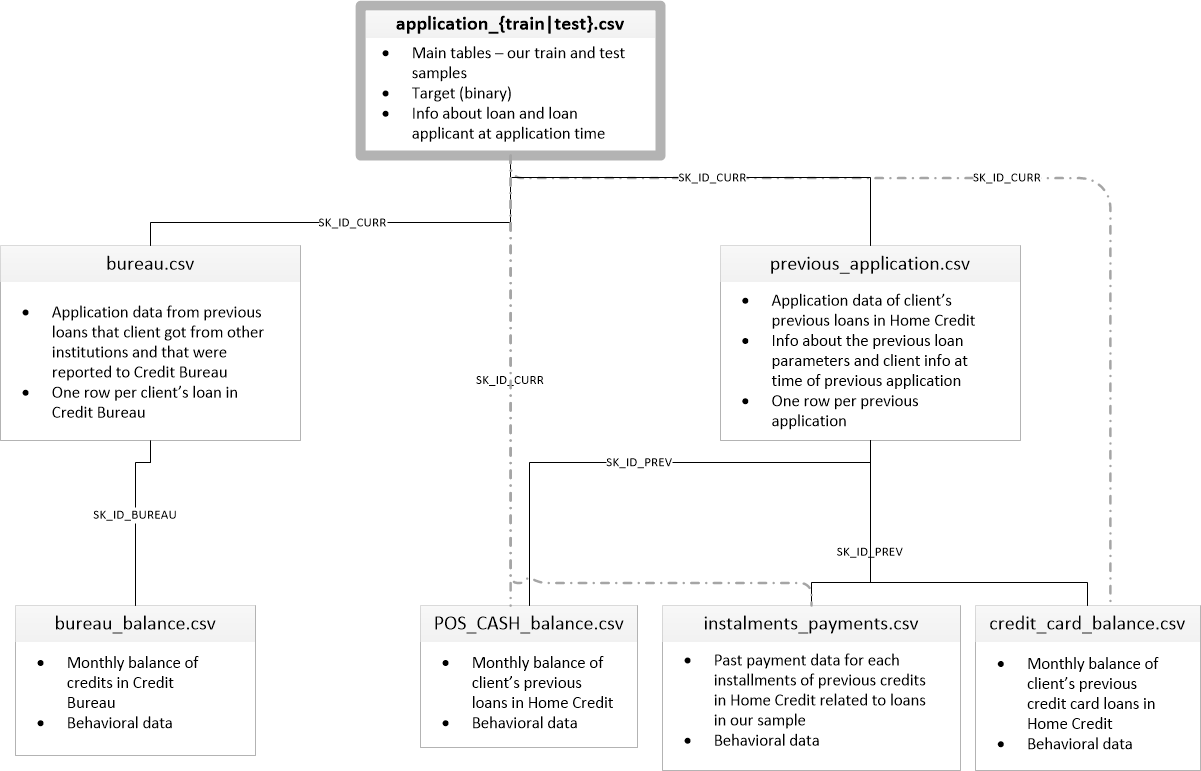
\includegraphics[width=0.9\textwidth]{homecredit}
\centering
\caption{Home Credit Data Table Relationships\cite{kagglehomecreditcompetitiondata}}
\end{figure}

\subsection{Problem Statement}
Home Credit needs an algorithm that will take as inputs various personal and financial information originally contained in a loan applicant's profile and structured as features in the seven data tables outlined above. The algorithm will then determine a probability of the applicant eventually making at least one late repayment on their loan. This probability will be in the range [0.0, 1.0], where 1.0 represents a 100\% certainty that the applicant will make at least one late repayment and 0.0 indicates that there is zero chance that the applicant will ever make a late payment. The algorithm will be tested on a set of 48,744 individuals who previously borrowed from Home Credit. Competition participants must submit a CSV file that contains one header row, and 48,744 prediction rows, where each prediction row contains both a user ID, the \colorbox{backcolor}{\textcolor{black}{\texttt{SKI_ID_CURR}}} column, and the probability, the \colorbox{backcolor}{\textcolor{black}{\texttt{TARGET}}} column, of that user being delinquent. The file must be formatted as follows:

\begin{lstlisting}
SK_ID_CURR,TARGET
100001,0.1
100005,0.9
100013,0.2
etc.
\end{lstlisting}

To solve this competition I intend to try out several machine learning algorithms that can also return the probabilities of their classification predictions, such as logistical regression and multi-layer perceptron classifiers. I will experiment with tuning hyperparameters both manually and automatically. I will train my algorithms using the 307,511 borrower records that comprise the training segment. However, since this is a Kaggle competition, Home Credit has removed the target data from the test set. This means that in order to guage the performance of the different algorithms I attempt to use, and in order to ensure that I don't overfit to the training data, it is imperative that I set aside a fraction of the training set (around 20\%) to serve as a validation test set. Alternatively, I could employ an algorithm such as K-Fold Cross Validation.

The seven data tables provided by Home Credit contain an awful lot of information that could take months to thoroughly investigate. So for the purposes of this project, I will focus on the features in the main data table. However, I will engineer at least one feature that is based on some portion of the data contained inside at least one of the other six tables. Finally, I will experiment with both manual and automatic feature selection.

Once I've finished my experimentation, I will choose the classifier/hyperparameter/feature combination that scores highest on my validation set and submit its test set probability predictions on the Kaggle competition's page. I am looking forward to seeing how my submission performs relative to other entries on the competition's leaderboard.

Home Credit knows which borrowers in the test set made at least one late loan payment, and which ones were never delinquent. The winning algorithm will therefore need to predict the highest probabilities of delinquency for the largest fraction of borrowers who did have at least one late payment, and will need to predict the lowest probabilities of delinquency for the largest fraction of borrowers who never had a late payment. More formally, a winning algorithm will have the highest true positive rate, or sensitivity, (correctly guessing who will be delinquent), while at the same time having a minimum false positive rate (as seldomly as possible making an incorrect guess that an individual would be delinquent).

\subsection{Metrics}
The area under the ROC (receiver operating characteristic) curve\cite{wikipediaroc} will be the evaluation metric for my solution to this competition. This area can range from a minimum value of 0, or 0\%, to a maximum of 1, or 100\%. The size of the area under an ROC curve indicates how good a job a classifier does of identifying, or separating out, a particular target segment from a dataset. An area of 1 indicates that the classifier is perfect -- that it can find every true positive (exhibiting perfect sensitivity, or recall) without making any mistakes (not accidentally labelling some true negatives as false positives), thus giving it perfect specificity, which leads to a false positive rate (1 - specificity), of zero. An area of 0 indicates that the classifier isn't able to find and properly label any of the true positives. An area of 0.5 is the level of performance we'd expect from a classifier that randomly labels each point in the dataset -- on the whole, this classifier would make just as many mistakes (false positives) as it makes correct predictions (true positives).

\begin{figure}[ht]
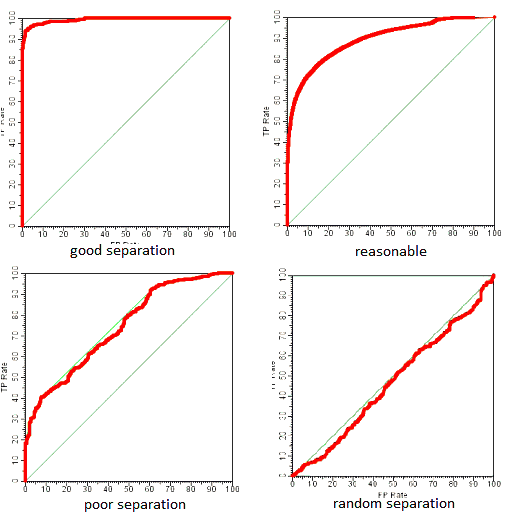
\includegraphics[width=0.5\textwidth]{roccurves}
\centering
\caption{ROC Curve Examples\cite{mlwikirocanalysis}}
\end{figure}

Because the goal of this competition is to create an algorithm that correctly identifies the target segment of loan applicants who will be delinquent in repaying their loans, the area under the ROC curve is a perfectly appropriate measure of my algorithm's performance. At a bare minimum, my classifier must achieve a score of better than 0.5 -- anything less would mean that my classifier performs only as good as, or worse than, a random classifier. A competition-winning solution will be the algorithm that has an area under its ROC curve that is closest to 1. This algorithm will naturally be able to correctly predict more delinquent repayers than the other submissions (maximizing the true positive rate), while at the same time making the fewest incorrect predictions about which applicants are delinquent repayers (minimizing the false positive rate).

\section{Analysis}
\subsection{Data Exploration}
\subsubsection{Data Table Statistics and Samples}
For this project I will make use of both the main data table (\colorbox{backcolor}{\textcolor{black}{\texttt{application_\{train \textbar~test\}.csv}}}) and the bureau data table (\colorbox{backcolor}{\textcolor{black}{\texttt{bureau.csv}}}). The main data table's training segment (\colorbox{backcolor}{\textcolor{black}{\texttt{application_train.csv}}}) contains 307,511 rows, each representing a unique individual who has previously borrowed money from Home Credit. The main data table contains 122 columns. The first two columns, \colorbox{backcolor}{\textcolor{black}{\texttt{SKI_ID_CURR}}} and \colorbox{backcolor}{\textcolor{black}{\texttt{TARGET}}}, represent a borrower's loan ID and target value, respectively. The loan ID is a unique identifier assigned to each borrower. A target value of 1 indicates that the borrower eventually made at least one late loan payment. A target value of 0 indicates that the borrower always paid on time. The remaining 120 columns contain features that encapsulate various information from a borrower's loan application profile. Features are both categorical and numerical. Some categorical features, such as gender (\colorbox{backcolor}{\textcolor{black}{\texttt{CODE_GENDER}}}), have not yet been one-hot encoded. Other categorical features, like whether or not the applicant submitted a mobile phone number (\colorbox{backcolor}{\textcolor{black}{\texttt{FLAG_MOBIL}}}), have been one-hot encoded. Some numerical features have been normalized and others have not. Most of the normalized features, such as the average number of entrances in a building, (\colorbox{backcolor}{\textcolor{black}{\texttt{ENTRANCES_AVG}}}), represent data about the applicant's building of residence. Non-normalized features often encapsulate general data on an applicant's employment and financial background, such as the number of days the applicant has had a job (\colorbox{backcolor}{\textcolor{black}{\texttt{DAYS_EMPLOYED}}}). A complete list of the main data table features in each of these categories can be seen in Appendix \ref{appendix:maindatatablefeaturetypes}.

Summary statistics of each numerical and previously one-hot encoded, now binary, categorical feature in the main data table's training set can be viewed in Appendix \ref{appendix:maindatatablestatsummary}. Samples of the first five entries for each of the features can be seen in Appendix \ref{appendix:maindatatablesamples}. Of the 307,511 applicants in the training segment, 282,686 people have a target value of 0 and 24,825 have a target value of 1. This means that roughly 8\% borrowers in the training set have made at least one late loan payment.

The main data table's testing segment (\colorbox{backcolor}{\textcolor{black}{\texttt{application_test.csv}}}) is identical in structure to \colorbox{backcolor}{\textcolor{black}{\texttt{application_train.csv}}}, save for the fact that the target information for the 48,744 borrowers in this segment has been removed. I will use my final, test validated learning algorithm to predict target values for the borrowers contained in this data table, and then submit these predictions on Kaggle.

The bureau data table (\colorbox{backcolor}{\textcolor{black}{\texttt{bureau.csv}}}) contains summary information of applicants' loans from other lenders, such as the amount and type of loan, as well as overdue repayment balance. Each row represents a unique loan. Many individual applicants have several rows in the bureau data table, where each row represents a different loan belonging to the same applicant. I will later engineer a feature based on one or more of the features contained in \colorbox{backcolor}{\textcolor{black}{\texttt{bureau.csv}}}. Appendix \ref{appendix:bureaudatatablestatsummary} contains statistical summaries of the numerical features in the bureau data table. Appendix \ref{appendix:bureaudatatablesamples} contains samples of the first five entries of all features.

\subsubsection{Main Data Table Features with `NaN' Entries}
The defining characteristic of the main data table is the prevalence of `NaN' entries. Over 67 of the 120 total features have one or more entries of `NaN'. Several of these features, especially ones containing numerical information on a borrower's residence building such as \colorbox{backcolor}{\textcolor{black}{\texttt{COMMONAREA_MEDI}}} and
\colorbox{backcolor}{\textcolor{black}{\texttt{NONLIVINGAPARTMENTS_AVG}}}, have nearly 70\% of their entries as `NaN'. Three questions drove my investigation of these 67 features:

\begin{enumerate}
  \item Might merely having `NaN' for a feature help predict a borrower's target value?
  \item Will features with numerous `NaN' entries even be useful at all?
  \item Do `NaN' values primarily belong to numerical features, categorical features, or both?
\end{enumerate}

\paragraph{Question 1:}
I confirmed that for all 67 features, a borrower simply having an `NaN' entry for a feature will not help predict whether the borrower will be more or less likely to be delinquent. I verified this by looking at the fractions of each feature's `NaN' and non-`NaN' cohorts that had a target value of 1. For each feature, I found that the fraction of `NaN' borrowers who were delinquent payers was identical to the fraction of non-`NaN' borrowers who were delinquent. If just having `NaN' for a particular feature were to have any chance of being a meaningful predictor of delinquency, I would have expected these two proportions to have had a stastically significant difference. Statistics summarizing `NaN' values for each feature can be viewed in Appendix \ref{appendix:maindatatablenanstatsummary}.

\paragraph{Question 2:}
It's helpful to remember that there are 24,825 borrowers in the training dataset who had a target value of 1. Any feature that I retain in spite of its `NaN' entries needs to have a large enough amount of non-`NaN' entries that belong to delinquent repayers. If the training set's delinquent population is not adequately represented among a particular feature's valid data points, it's unlikely that a prediction algorithm trained on this feature would generalize well to unseen datapoints. The effective size of the feature's training set would be too small, and the model would be at risk of underfitting.

However, what should the cutoff line be? What fraction of the 24,825 delinquent borrowers need to be represented by a feature's valid data points in order for the feature to be useful for making predictions? There is no general rule of thumb and the short answer is that it depends -- on many factors such as the distribution of the feature's valid data, as well as the type of learning algorithm I'm using.

Thus for the time being I decided not to remove any of these features -- even features like \colorbox{backcolor}{\textcolor{black}{\texttt{COMMONAREA_MEDI}}} that contain `NaN' in over two-thirds of their entries. Instead of running detailed statistical analyses on these features' distributions, I will instead experiment with dimensionality reduction algorithms such as PCA and/or feature selection algorithms such as SelectKBest.

If a feature had 95\% of its entries as `NaN', I would have removed it from the dataset at this point. However, since the sparsest features in the main data table still have valid data in just over 30\% of their entries, I don't want to prematurely remove a feature that may have a chance, however remote, of contributing to useful predictions.

\paragraph{Question 3:}
I found that all but one of the 47 normalized numerical features contain `NaN' values. About half of the 21 non-normalized numerical features contain `NaN' entries. Only three out of the 15 categorical features that will need to be one-hot encoded contain `NaN' entries. None of the already one-hot encoded categorical features contain `NaN' entries. See Appendix \ref{appendix:maindatatablefeaturetypes}.

\subsubsection{Main Data Table Borrowers with `NaN' Entries}
I investigated whether any borrowers had `NaN' entries for nearly all of their feature data -- could any borrowers be removed from the training set because their feature data is too sparse?

\begin{figure}[ht]
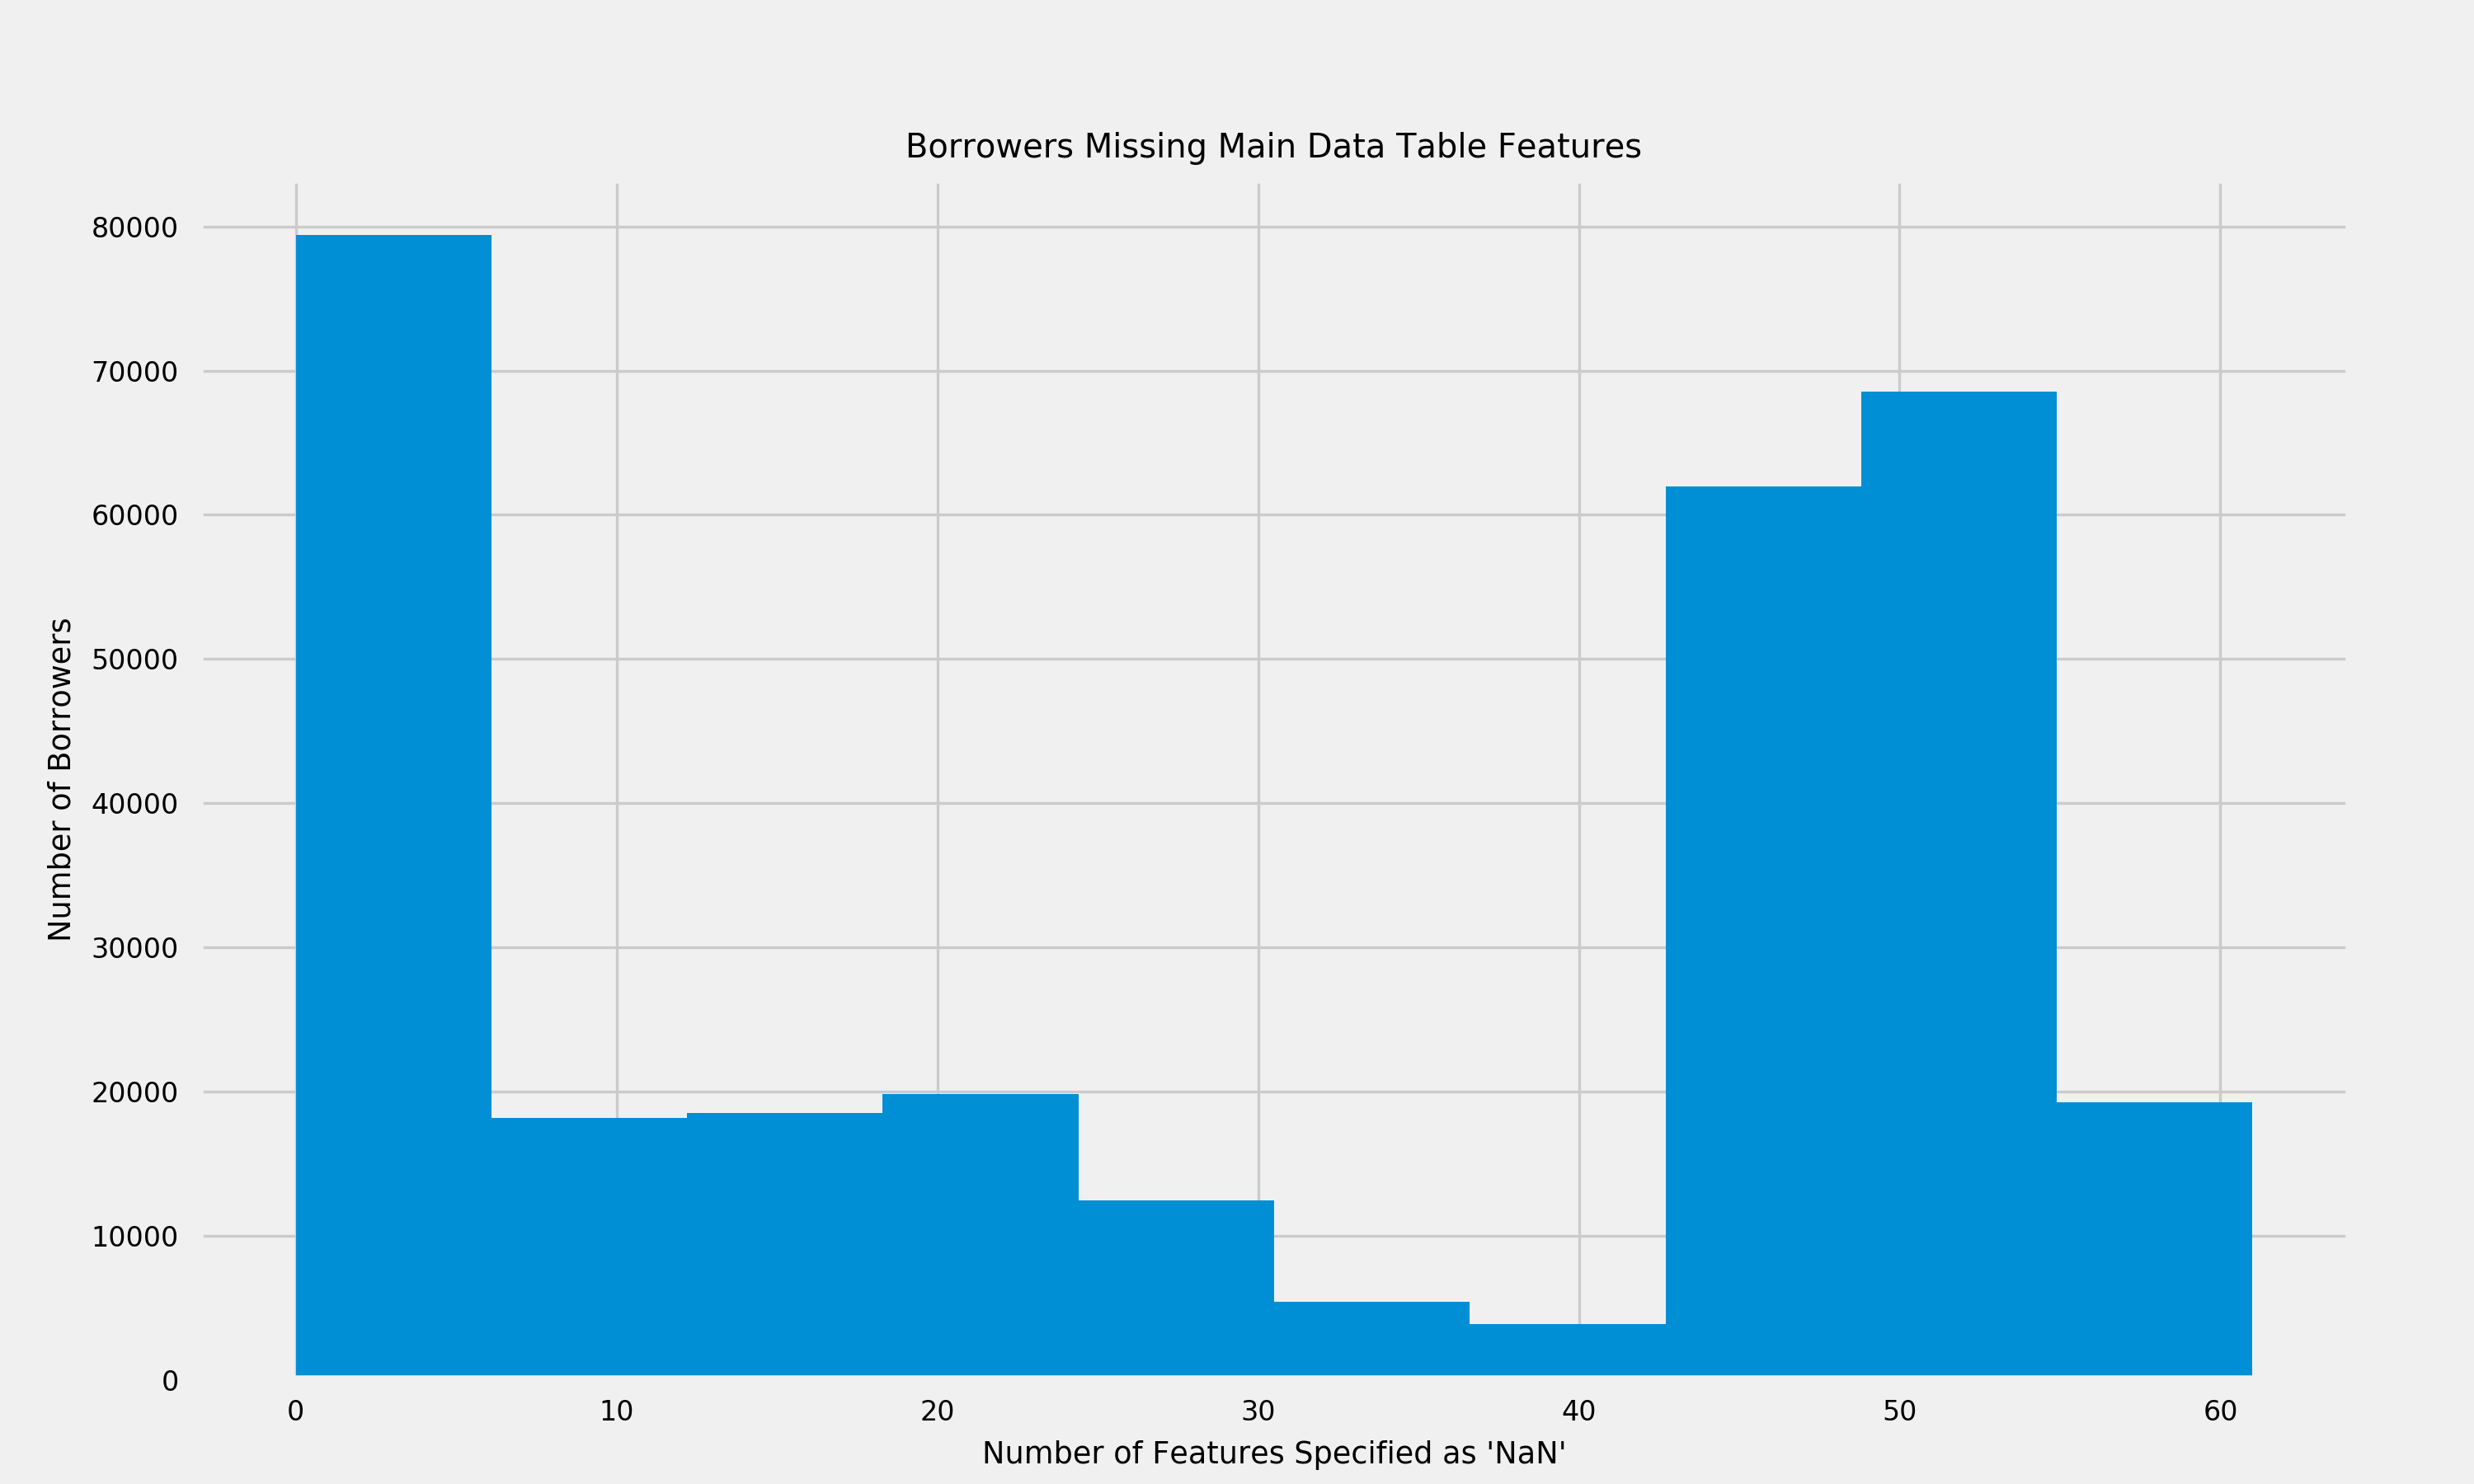
\includegraphics[width=0.7\textwidth]{borrowersnandata}
\centering
\caption{Borrowers Missing Main Data Table Features}
\end{figure}

The above plot confirms that no borrowers are missing data for so many features such that they'd be considered outliers. At it is, a borrower could at most be missing roughly only half of the main data table's 120 features. Just under 20,000 of the training dataset's 307,511 borrower records face this "worst-case" scenario. A borrower would have to be missing well over 100 features, or at least five-sixths of the main data table featureset, before I would consider removing them. Becauase these 20,000 borrowers have valid entries for half of the dataset's features, I believe there is a greater chance that they will be valuable training points for my learning algorithm, as opposed to being unhelpful noise.

\subsubsection{Main Data Table Anomalies}
I explored data samples\ref{appendix:maindatatablesamples} and statistical descriptions\ref{appendix:maindatatablestatsummary} of the main data table to ensure that no features contained unexpected values that fall outside the range one would expect based on the feature's definition. Examples of unexpected values include entries that are impossibly small/large, or values that are negative when only positive values would be expected.I came across the following five anomalies.

\paragraph{Anomaly 1:}
The five numerical features, \colorbox{backcolor}{\textcolor{black}{\texttt{DAYS_BIRTH}}}, \colorbox{backcolor}{\textcolor{black}{\texttt{DAYS_EMPLOYED}}}, \colorbox{backcolor}{\textcolor{black}{\texttt{DAYS_REGISTRATION}}}, \colorbox{backcolor}{\textcolor{black}{\texttt{DAYS_ID_PUBLISH}}}, and \colorbox{backcolor}{\textcolor{black}{\texttt{DAYS_LAST_PHONE_CHANGE}}}, indicate the number of days prior to the loan application's submission that a particular event took place. For example, \colorbox{backcolor}{\textcolor{black}{\texttt{DAYS_LAST_PHONE_CHANGE}}} is defined by Home Credit as being the number of days before their loan application that the applicant last changed their phone number.

Values for the above five features are negative, which is expected since each value represents a point in time prior to the time of the loan application's submission, which Home Credit defines as time 0.

What's unexpected is that the \colorbox{backcolor}{\textcolor{black}{\texttt{DAYS_EMPLOYED}}} feature (the number of days an applicant has had a job prior to submitting their application) has a maximum value that is both a \textit{positive} number as well as \textit{unbelievably large}. This maximum value is 365,243 days, or just over 1,000 years!

No human being lives for 1,000 years, let alone holds a job for that long, so this entry clearly indicates a mistake or a special case. What wasn't clear to me was whether \colorbox{backcolor}{\textcolor{black}{\texttt{DAYS_EMPLOYED}}} contains only one, a few, or several similar entries. Inspecting a histogram of this feature's data should help me answer this question. My intuition tells me that all things being equal, \colorbox{backcolor}{\textcolor{black}{\texttt{DAYS_EMPLOYED}}} could be useful in predicting borrowers' target values, if I can figure out how to handle these outliers.

\paragraph{Anomaly 2:}
I was undecided whether the features \colorbox{backcolor}{\textcolor{black}{\texttt{OWN_CAR_AGE}}}, the age of the applicant's car,  \colorbox{backcolor}{\textcolor{black}{\texttt{HOUR_APPR_PROCESS_START}}}, the hour the loan application was submitted, \colorbox{backcolor}{\textcolor{black}{\texttt{CNT_CHILDREN}}}, the number of children that the applicant has, and \colorbox{backcolor}{\textcolor{black}{\texttt{CNT_FAM_MEMBERS}}}, the size of the applicant's family, should be thought of as categorical or numerical.

This was because the entries for each feature are rounded to whole numbers and their ranges are quite small: [0,23] for \colorbox{backcolor}{\textcolor{black}{\texttt{HOUR_APPR_PROCESS_START}}}, [0.0,91.0] for \colorbox{backcolor}{\textcolor{black}{\texttt{OWN_CAR_AGE}}}, [0.0,19.0] for \colorbox{backcolor}{\textcolor{black}{\texttt{CNT_CHILDREN}}}, and [1.0,20.0] for \colorbox{backcolor}{\textcolor{black}{\texttt{CNT_FAM_MEMBERS}}}.

I noticed that other categorical features in the main data table, such as whether the applicant owns a car, or the applicant's housing type, each have distinct entries that encapsulate wildly different meanings. The condition of owning a car, for example, is very different from the condition of not owning a car. After thinking along these lines, it was easy for me to see that neither the entries in \colorbox{backcolor}{\textcolor{black}{\texttt{OWN_CAR_AGE}}} nor those \colorbox{backcolor}{\textcolor{black}{\texttt{HOUR_APPR_PROCESS_START}}} are necessarily always that different from one another in meaning or implication. Is submitting a loan application at 3PM really that different from submitting at 4PM? It is far more likely that there are meaningful sub-ranges, such as the afternoon hours of 1PM to 5PM, that may be helpful in predicting a borrower's target value. It's best to treat these two features as numerical in order to discover the most meaningful sub-ranges.

Things are different for the \colorbox{backcolor}{\textcolor{black}{\texttt{CNT_CHILDREN}}} and \colorbox{backcolor}{\textcolor{black}{\texttt{CNT_FAM_MEMBERS}}} features. Although the most children any loan applicant had was 19, at least 75\% of all applicants had either zero children or just one child. I decided that it makes most sense to treat  \colorbox{backcolor}{\textcolor{black}{\texttt{CNT_CHILDREN}}} as a categorical feature, and re-engineer it to segment the borrower population into the following two categories: having no children, and having one or more children. Although I expect there will groups of borrowers of diminishing size that have 2,3,4,...,19 children, my hypothesis is that having no children versus having at least one child will be the information most useful to predict target values for the overall population of borrowers. Even if I were to spend time investigating the effects of having 2 vs. 3 vs. 4 vs. ... vs. 19 children, I know that my findings would apply to less than 25\% of the overall population and any predictions informed by these effects likely wouldn't generalize well to unseen datapoints.

I will transform the \colorbox{backcolor}{\textcolor{black}{\texttt{CNT_CHILDREN}}} feature into a binary categorical feature called \colorbox{backcolor}{\textcolor{black}{\texttt{HAS_CHILDREN}}}. If the value of \colorbox{backcolor}{\textcolor{black}{\texttt{CNT_CHILDREN}}} is greater than 0, the value of \colorbox{backcolor}{\textcolor{black}{\texttt{HAS_CHILDREN}}} will be 1. If the value of \colorbox{backcolor}{\textcolor{black}{\texttt{CNT_CHILDREN}}} is 0, the value of \colorbox{backcolor}{\textcolor{black}{\texttt{HAS_CHILDREN}}} will be 0.

For \colorbox{backcolor}{\textcolor{black}{\texttt{CNT_FAM_MEMBERS}}}, the situation is somewhat similar. 25\% of borrowers in the training set have a family size of just one, 50\% have a family of two or less, and 75\% of borrowers have families of 3 people or less. I plan to re-engineer this feature to categorically segment borrowers into the following three groups: having a family size of one, a family size of two, and having a family that's three people or larger.

I will transform the \colorbox{backcolor}{\textcolor{black}{\texttt{CNT_FAM_MEMBERS}}} feature into a categorical feature called \colorbox{backcolor}{\textcolor{black}{\texttt{NUMBER_FAMILY_MEMBERS}}}. If \colorbox{backcolor}{\textcolor{black}{\texttt{CNT_FAM_MEMBERS}}} is 1.0, then the value of \colorbox{backcolor}{\textcolor{black}{\texttt{NUMBER_FAMILY_MEMBERS}}} will be `one'. If \colorbox{backcolor}{\textcolor{black}{\texttt{CNT_FAM_MEMBERS}}} is 2.0, then \colorbox{backcolor}{\textcolor{black}{\texttt{NUMBER_FAMILY_MEMBERS}}} will be `two'. If \colorbox{backcolor}{\textcolor{black}{\texttt{CNT_FAM_MEMBERS}}} is 3.0 or greater, then \colorbox{backcolor}{\textcolor{black}{\texttt{NUMBER_FAMILY_MEMBERS}}} will be `three_plus'. The new categorical feature \colorbox{backcolor}{\textcolor{black}{\texttt{NUMBER_FAMILY_MEMBERS}}} will eventually be one-hot encoded.

\paragraph{Anomaly 3:}
While most features reported as being normalized have a max value of 1.0 and a min value of 0.0. The features \colorbox{backcolor}{\textcolor{black}{\texttt{EXT_SOURCE_1}}}, \colorbox{backcolor}{\textcolor{black}{\texttt{EXT_SOURCE_2}}}, and \colorbox{backcolor}{\textcolor{black}{\texttt{EXT_SOURCE_3}}} all have values within the range (0.0, 1.0), none of them have maximums of 1.0, nor minimums of 0.0. Because of this discrepancy I will pay special attention to the graphs of these features' distributions when conducting my exploratory data visualization.

\paragraph{Anomaly 4:}
The feature \colorbox{backcolor}{\textcolor{black}{\texttt{REGION_POPULATION_RELATIVE}}} is unique in that while it is identified as normalized, its values only fall into the range [0.000290, 0.072508]. All other normalized features were scaled to the range [0.0,1.0]. It's a given that I'll need to scale this feature to [0.0,1.0] during data preprocessing.

\paragraph{Anomaly 5:}
The four features \colorbox{backcolor}{\textcolor{black}{\texttt{FONDKAPREMONT_MODE}}}, \colorbox{backcolor}{\textcolor{black}{\texttt{HOUSETYPE_MODE}}}, \colorbox{backcolor}{\textcolor{black}{\texttt{WALLSMATERIAL_MODE}}}, and \colorbox{backcolor}{\textcolor{black}{\texttt{EMERGENCYSTATE_MODE}}} were described by Home Credit as normalized. However, I found that each of these four features was in fact categorical, and would need to be one-hot encoded. \colorbox{backcolor}{\textcolor{black}{\texttt{WALLSMATERIAL_MODE}}}, for example, contains entries such as ``Stone, brick", ``panel", and ``block" that indicate the material(s) of which the walls in the borrower's house are built.

\subsubsection{Feature Engineering}
Of the six tables in the dataset aside from the main data table, four tables (\colorbox{backcolor}{\textcolor{black}{\texttt{previous_application.csv}}}, \colorbox{backcolor}{\textcolor{black}{\texttt{POS_CASH_balance.csv}}}, \colorbox{backcolor}{\textcolor{black}{\texttt{installments_payments.csv}}}, and \colorbox{backcolor}{\textcolor{black}{\texttt{credit_card_balance.csv}}}) contain information pertaining to previous applications and payback histories on prior loans that an applicant has had with Home Credit.

\colorbox{backcolor}{\textcolor{black}{\texttt{bureau.csv}}}, on the other hand, contains summary information of applicants' loans from \textit{other} lenders, such as the amount and type of loan, and any repayment balance that's overdue\ref{bureaudatatablefeatures}. \colorbox{backcolor}{\textcolor{black}{\texttt{bureau_balance.csv}}} contains month-by-month statuses for each loan recorded in bureau.csv that indicate whether a particular month's balance payment was received and processed\ref{bureaubalancedatatablefeatures}.

My hypothesis is that it will be most useful to engineer a feature that contains information about applicants' most recent payment performance on loans received from lenders other than Home Credit. The \colorbox{backcolor}{\textcolor{black}{\texttt{CREDIT_DAY_OVERDUE}}} feature in \colorbox{backcolor}{\textcolor{black}{\texttt{bureau.csv}}} gives the number of days that an individual's loan's payments have been overdue.

For simplicity's sake, my engineered feature will be built on \colorbox{backcolor}{\textcolor{black}{\texttt{CREDIT_DAY_OVERDUE}}}, and will indicate whether or not a Home Credit applicant currently has overdue loan payments from other creditors.

My engineered feature will be titled \colorbox{backcolor}{\textcolor{black}{\texttt{HAS_CREDIT_BUREAU_LOANS_OVERDUE}}}. If a Home Credit applicant has at least one loan in \colorbox{backcolor}{\textcolor{black}{\texttt{bureau.csv}}} for which \colorbox{backcolor}{\textcolor{black}{\texttt{CREDIT_DAY_OVERDUE}}} has a value greater than 0, the value of my new feature applicant will be 1. Otherwise, the value will be 0. Once the feature has been created, I will append it to the main data table.

\subsection{Exploratory Visualization}
\subsubsection{Distributions of Main Data Table Numerical Features Identified as Normalized}
I plotted distributions of 47 numerical features that Home Credit had identified as normalized. I ignored all `NaN' entries. All 47 plots can be viewed in Appendix \ref{normalfeaturedistribs}. I paid special attention to the distributions of four features I had found anomalous while exploring the dataset: \colorbox{backcolor}{\textcolor{black}{\texttt{EXT_SOURCE_1}}}, \colorbox{backcolor}{\textcolor{black}{\texttt{EXT_SOURCE_2}}}, \colorbox{backcolor}{\textcolor{black}{\texttt{EXT_SOURCE_3}}}, and \colorbox{backcolor}{\textcolor{black}{\texttt{REGION_POPULATION_RELATIVE}}}.

\begin{figure}[ht]
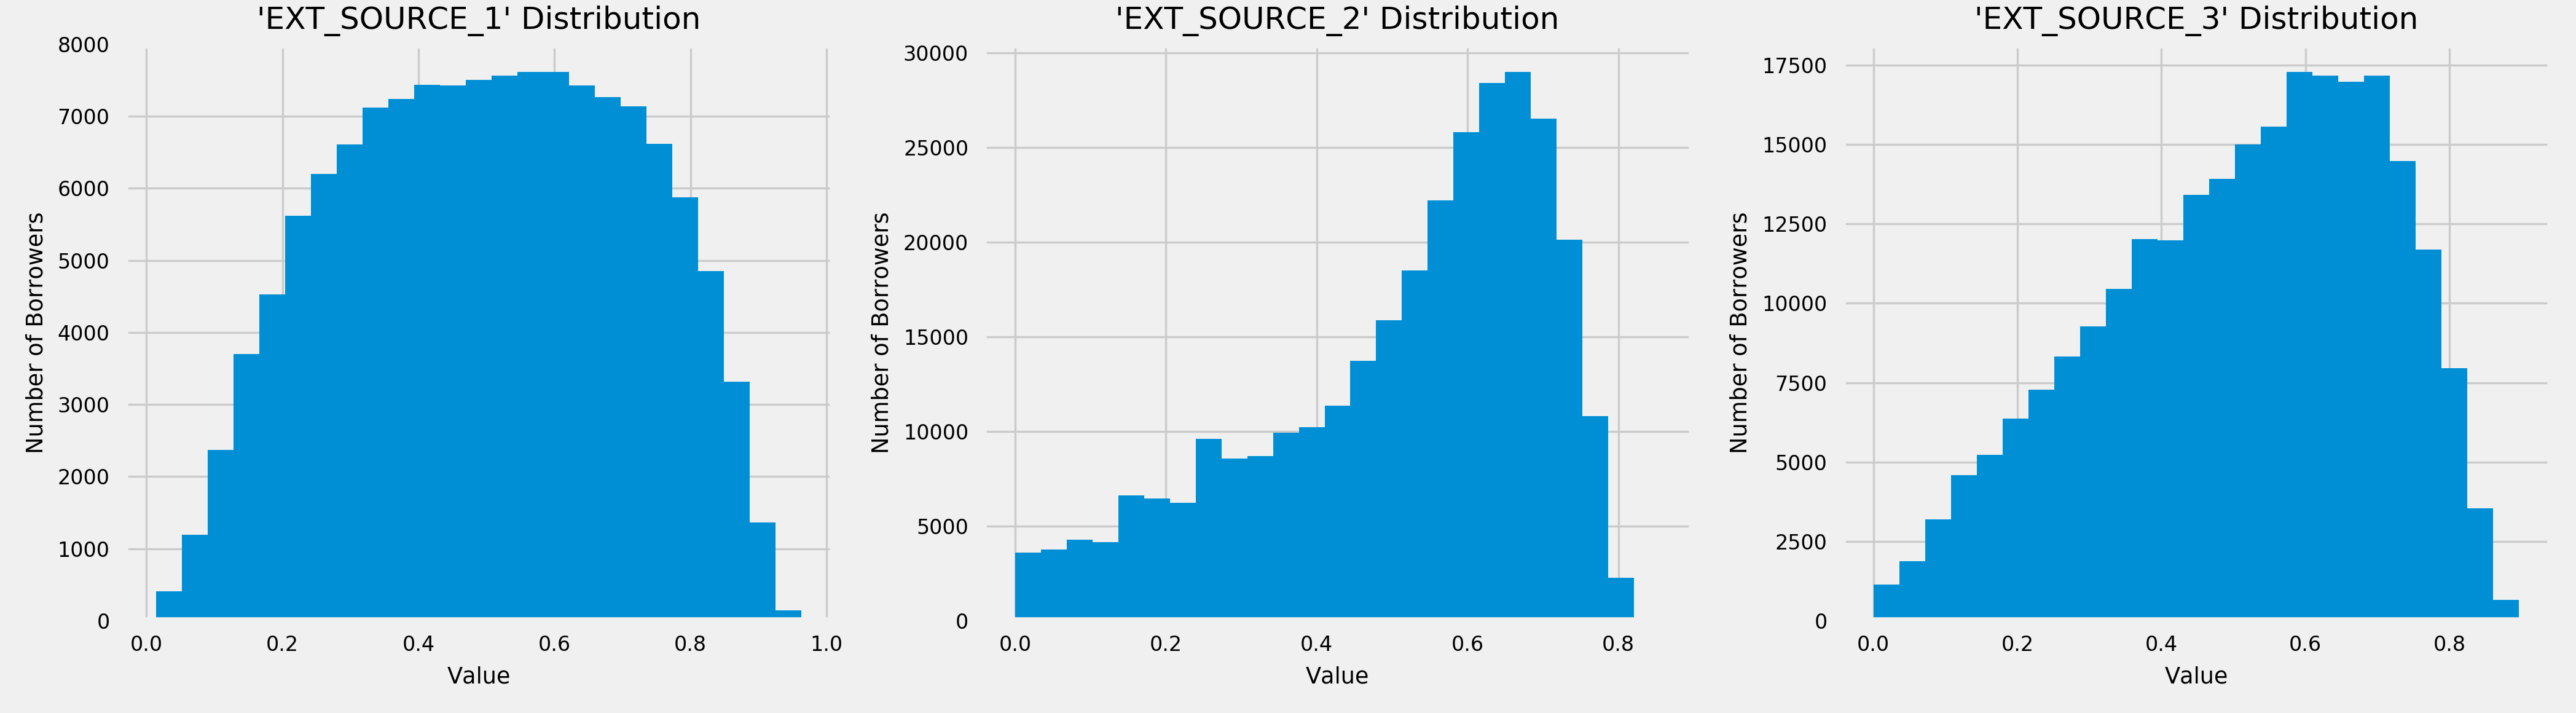
\includegraphics[width=\textwidth]{distribsEXTSOURCE1EXTSOURCE2EXTSOURCE3}
\centering
\caption{Distributions of Features \colorbox{backcolor}{\textcolor{black}{\texttt{EXT_SOURCE_1}}}, \colorbox{backcolor}{\textcolor{black}{\texttt{EXT_SOURCE_2}}}, \colorbox{backcolor}{\textcolor{black}{\texttt{EXT_SOURCE_3}}}}
\end{figure}

It turned out that \colorbox{backcolor}{\textcolor{black}{\texttt{EXT_SOURCE_1}}}, \colorbox{backcolor}{\textcolor{black}{\texttt{EXT_SOURCE_2}}}, and \colorbox{backcolor}{\textcolor{black}{\texttt{EXT_SOURCE_3}}} were the three features I should have been least concerned about. The shapes of these features' distributions more closely a the normal bell curve than all other normalized numerical features. And perhaps this shouldn't have been so surprising. According to Home Credit's definitions, these three features represent normalized scores that came from an "external data source," and I can only surmise that whatever methodology the external source used to define and assign these scores may be what results in their values being more normally distributed across the training dataset.

\begin{figure}[ht]
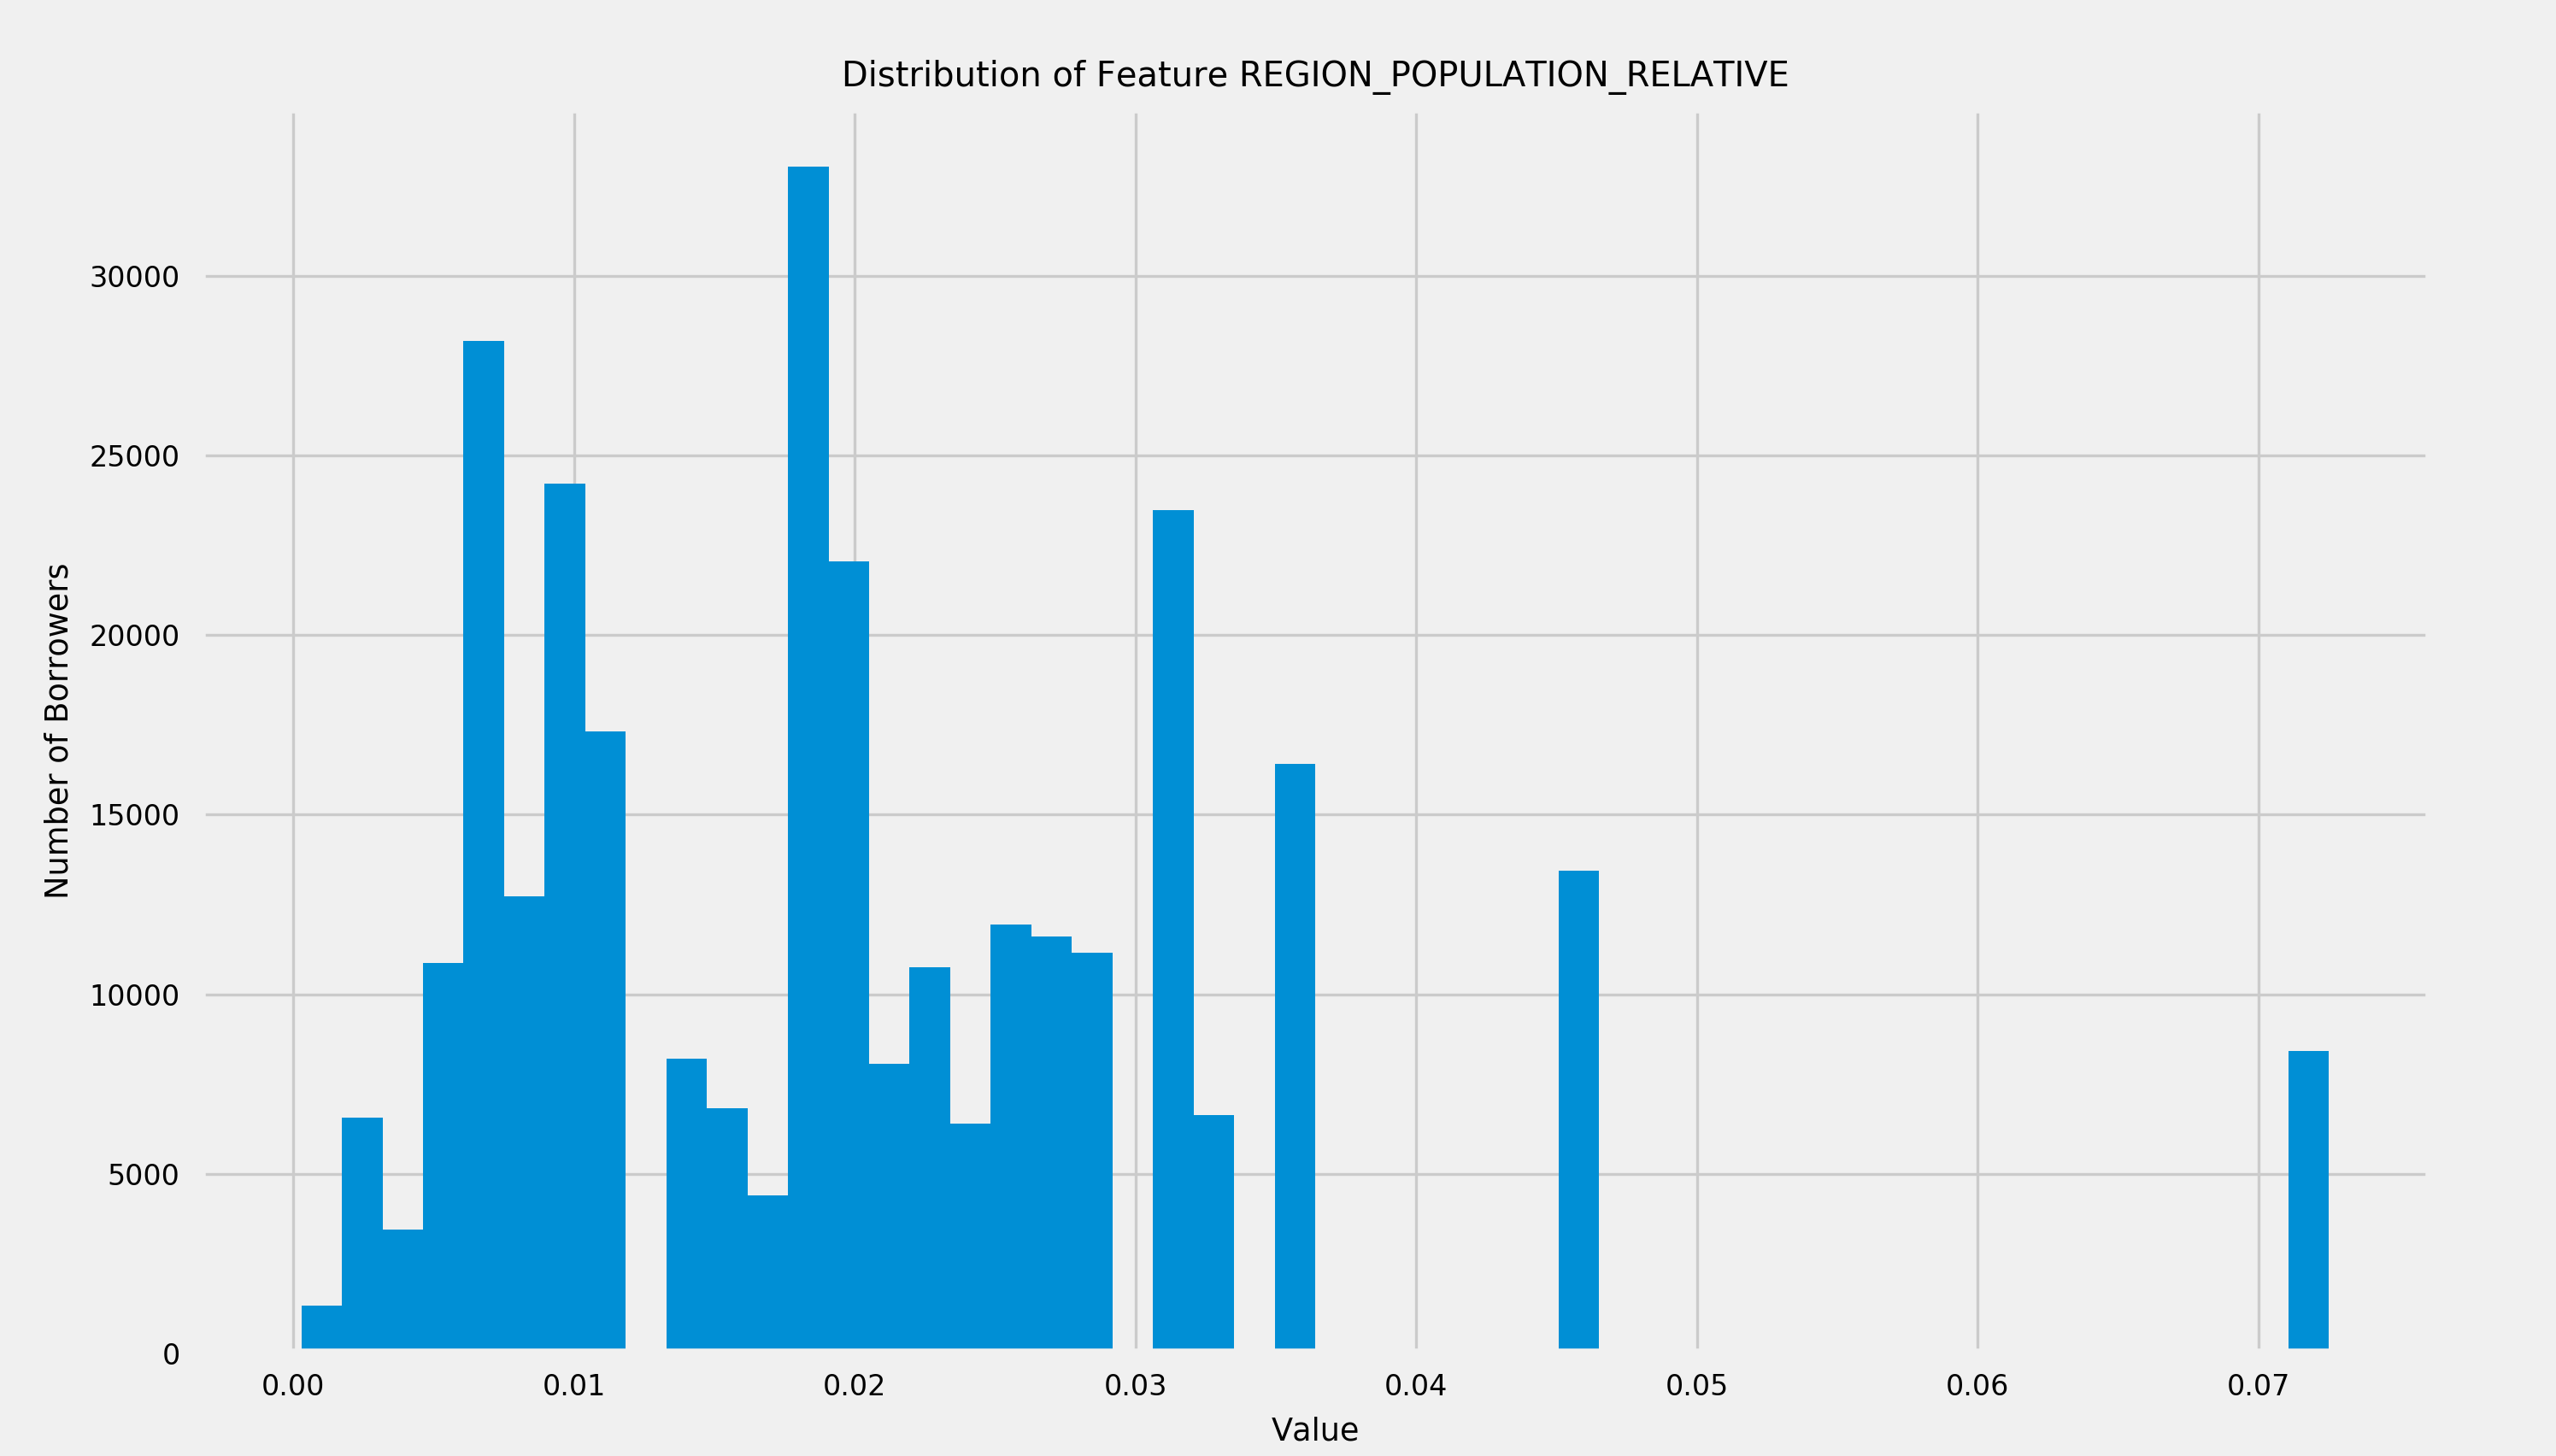
\includegraphics[width=0.7\textwidth]{distribREGIONPOPULATIONRELATIVE}
\centering
\caption{Distribution of Feature \colorbox{backcolor}{\textcolor{black}{\texttt{REGION_POPULATION_RELATIVE}}}}
\end{figure}

The feature \colorbox{backcolor}{\textcolor{black}{\texttt{REGION_POPULATION_RELATIVE}}} does indeed have all its values within an approximate range of [0.00,0.07]. There is nothing in the feature's definition that suggests why, out of all the other normalized features, this is the only feature not scaled to the range [0.0,1.0]. Thankfully, this feature exhibits minimal positive or negative skewness. The only preprocessing necessary is scale this feature to the range [0.0,1.0].

\begin{figure}[ht]
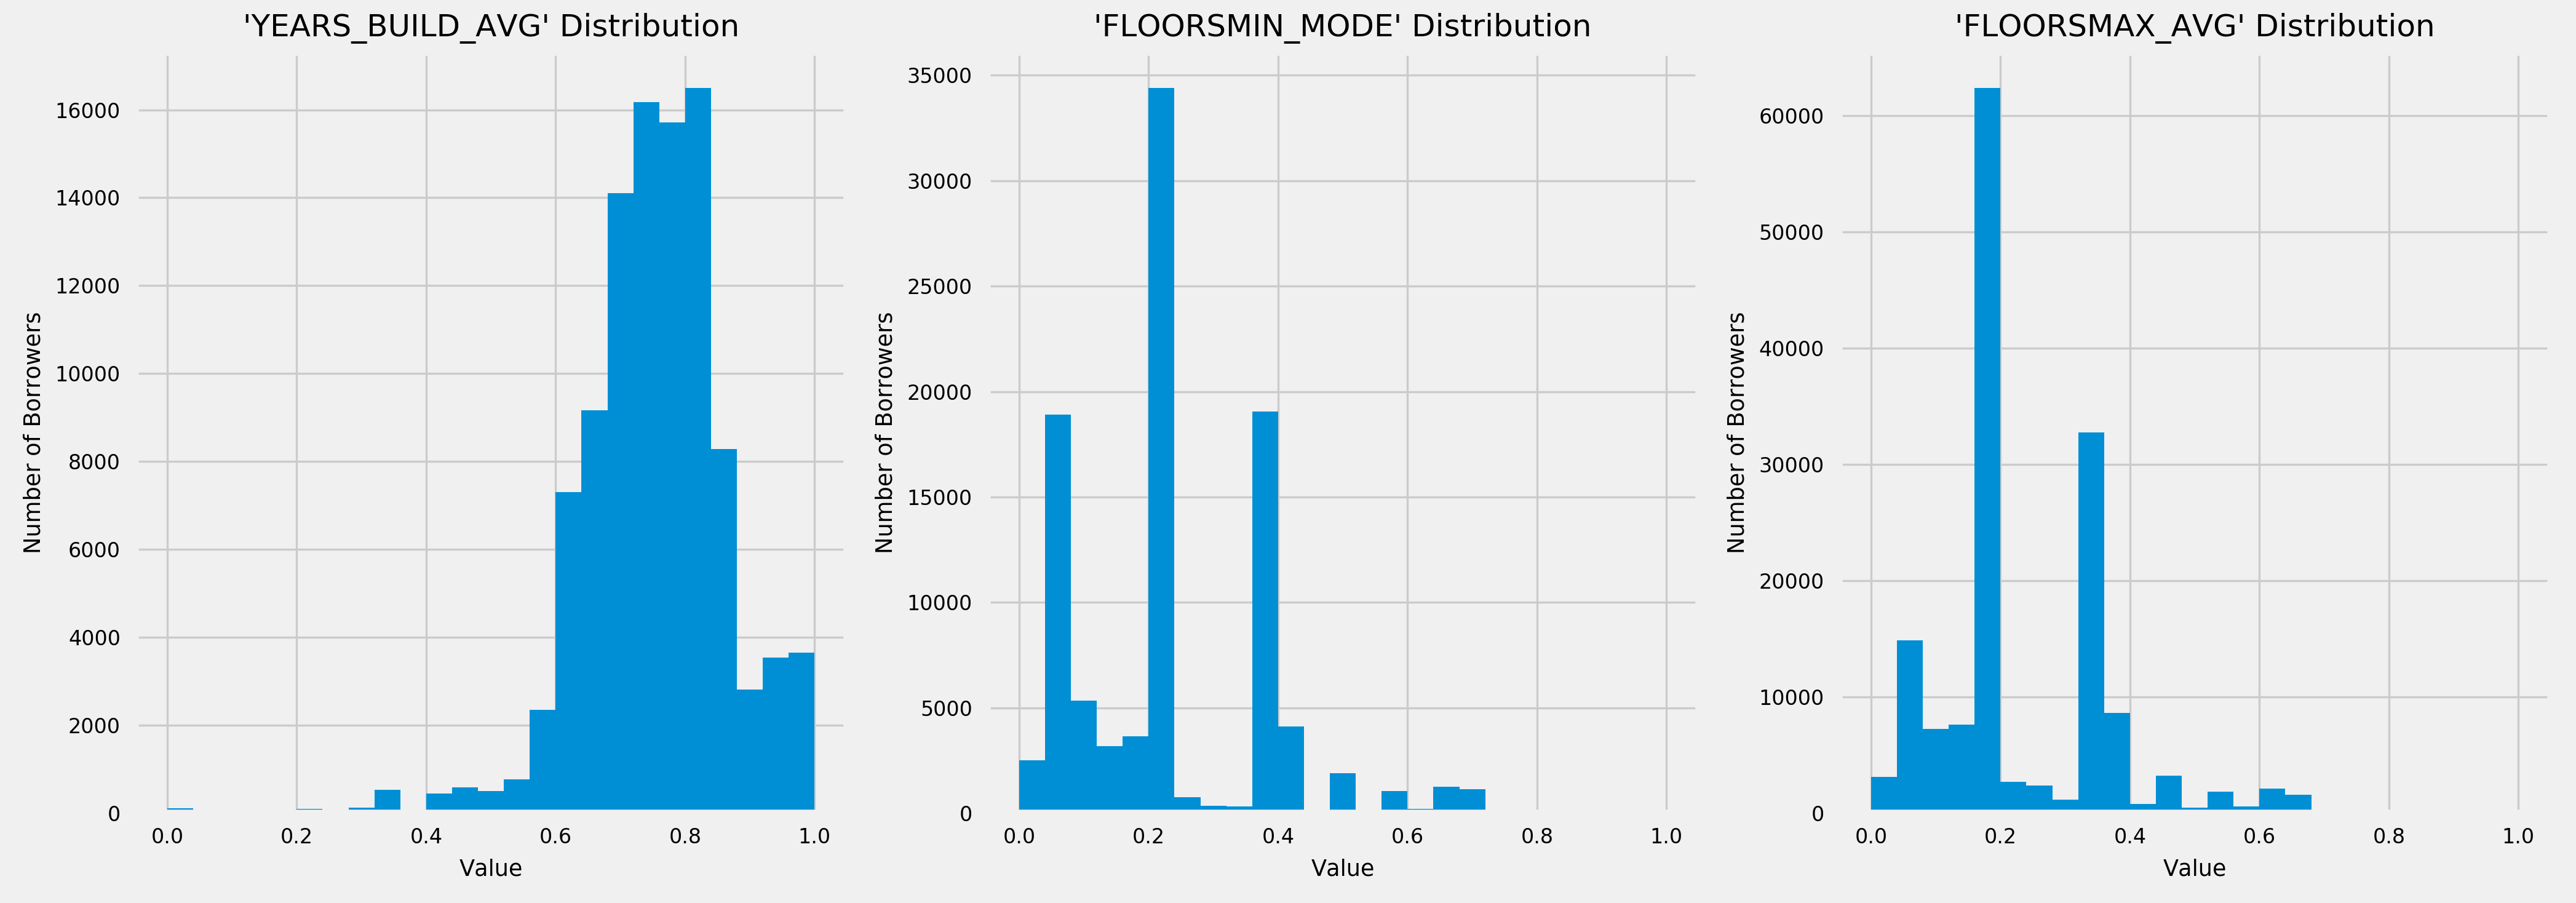
\includegraphics[width=\textwidth]{distribsYEARSBUILDAVGFLOORSMINMODEFLOORSMAXAVG}
\centering
\caption{Distributions of Features \colorbox{backcolor}{\textcolor{black}{\texttt{YEARS_BUILD_AVG}}}, \colorbox{backcolor}{\textcolor{black}{\texttt{FLOORSMIN_MODE}}}, \colorbox{backcolor}{\textcolor{black}{\texttt{FLOORSMAX_AVG}}}}
\end{figure}

Normalized features describing general qualities of a borrower's residence that would apply to any building type also had a normal appearance without much positive or negative skewness. Such features include \colorbox{backcolor}{\textcolor{black}{\texttt{YEARS_BUILD_AVG}}}, \colorbox{backcolor}{\textcolor{black}{\texttt{FLOORSMIN_MODE}}}, and \colorbox{backcolor}{\textcolor{black}{\texttt{FLOORSMAX_AVG}}}, which indicate the year the residence was built and measures of number of floors, respectively.

\begin{figure}[ht]
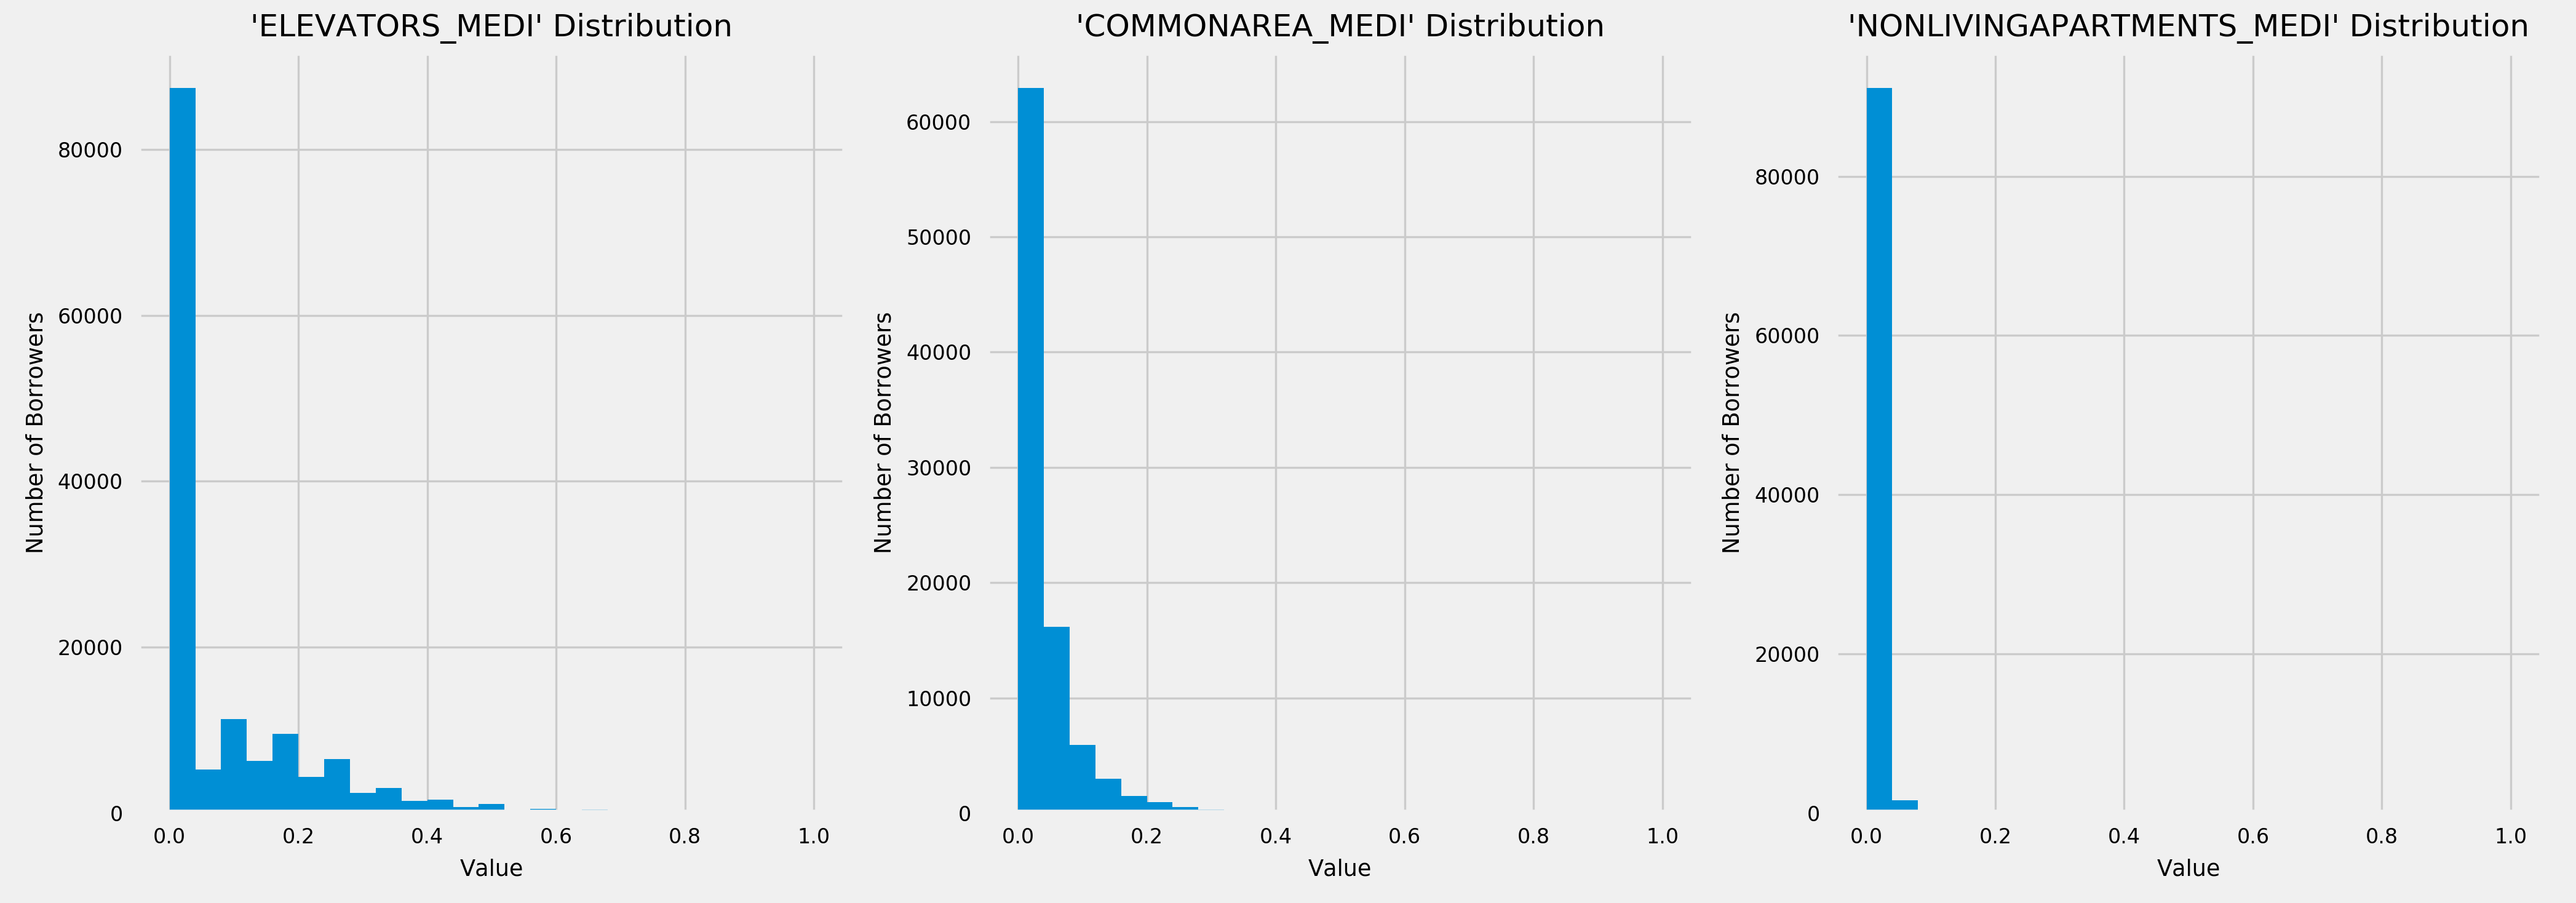
\includegraphics[width=\textwidth]{distribsELEVATORSMEDICOMMONAREAMEDINONLIVINGAPARTMENTSMED}
\centering
\caption{Distributions of Features \colorbox{backcolor}{\textcolor{black}{\texttt{ELEVATORS_MEDI}}}, \colorbox{backcolor}{\textcolor{black}{\texttt{COMMONAREA_MEDI}}}, \colorbox{backcolor}{\textcolor{black}{\texttt{NONLIVINGAPARTMENTS_MEDI}}}}
\end{figure}

On the other hand, the remaining normalized features, such as \colorbox{backcolor}{\textcolor{black}{\texttt{ELEVATORS_MEDI}}}, \colorbox{backcolor}{\textcolor{black}{\texttt{COMMONAREA_MEDI}}}, \colorbox{backcolor}{\textcolor{black}{\texttt{NONLIVINGAPARTMENTS_MEDI}}}, describe more niche characteristics of a residence building that may not apply to many borrowers in the training set. For example, individuals who live in a house wouldn't be expected to have any elevators, a public common area, or non-living apartments in their residence. Even though these features have been normalized, they tend to be noticeably positively skewed. Nonetheless, because these features are identified as having already been ``normalized," I will not attempt to further log-normalize these features -- due to the nature of these features' values, their distributions are likely already as ``normal" as they can possibly get.

\subsubsection{Distributions of Main Data Table Numerical Features Identified as Non-Normalized}
I also plotted histograms of 21 numerical features that were not identified by Home Credit as being normalized, in order to observe their skewness and discover which ones would be candidates for log-normalization. All 21 plots can be viewed in Appendix \ref{nonnormalfeaturedistribs}. All of these 21 features will need to be scaled to a range of [0.0,1.0]. All but three features are good candidates for log-normalization -- especially features having most values concentrated near zero and a smattering of large-valued outliers. Log-normalization may prevent the wide gulfs between these features' very large and small values from hindering a learning algorithm's performance.

Interestingly, the features \colorbox{backcolor}{\textcolor{black}{\texttt{DAYS_BIRTH}}}, \colorbox{backcolor}{\textcolor{black}{\texttt{DAYS_ID_PUBLISH}}}, and \colorbox{backcolor}{\textcolor{black}{\texttt{HOUR_APPR_PROCESS_START}}} already have non-skewed, normal shaped distributions. It will not be necessary for them to be log-normalized.

\pagebreak

\begin{figure}[h!]
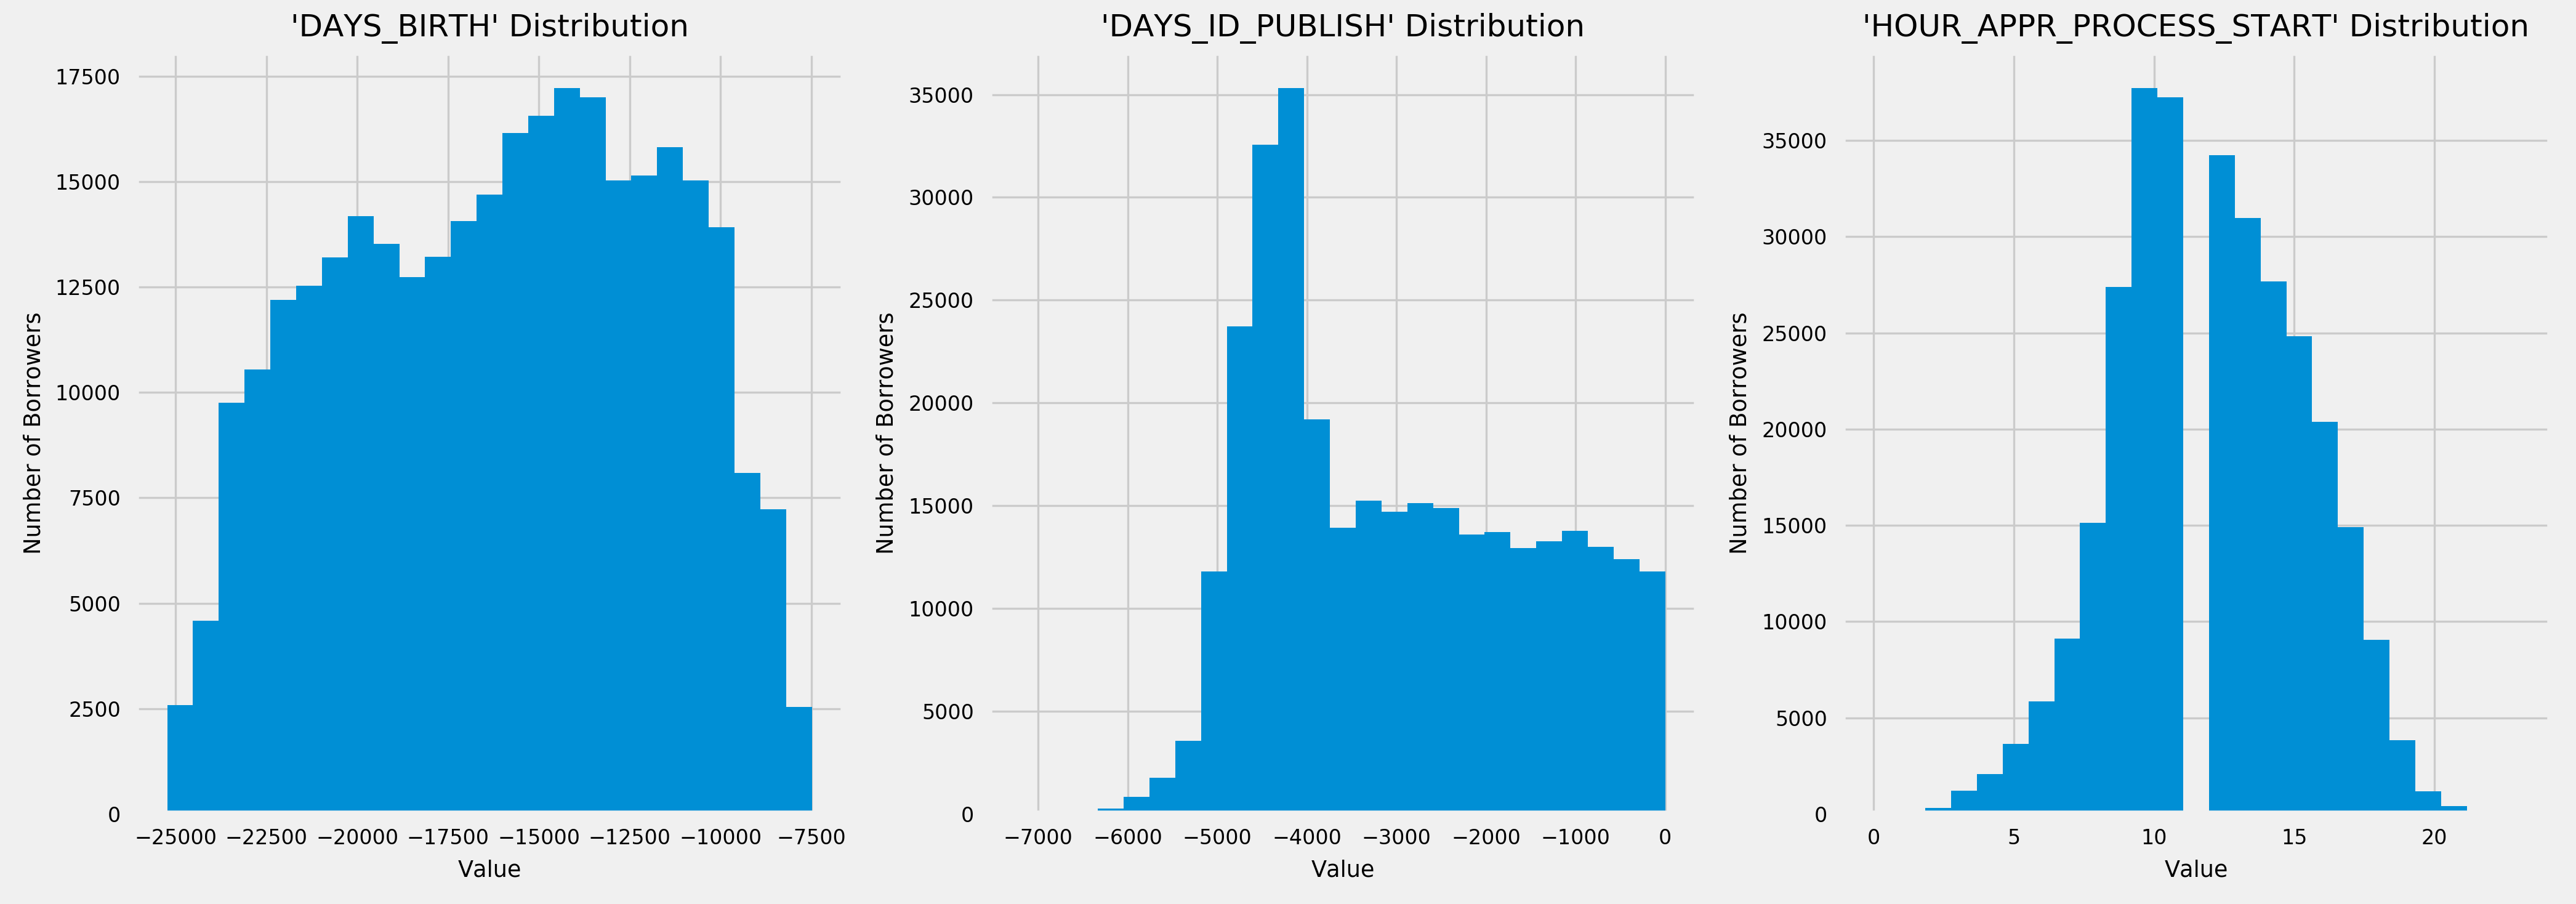
\includegraphics[width=\textwidth]{distribsDAYSBIRTHDAYSIDPUBLISHHOURAPPRPROCESSSTART}
\centering
\caption{Distributions of Features \colorbox{backcolor}{\textcolor{black}{\texttt{DAYS_BIRTH}}}, \colorbox{backcolor}{\textcolor{black}{\texttt{DAYS_ID_PUBLISH}}}, \colorbox{backcolor}{\textcolor{black}{\texttt{HOUR_APPR_PROCESS_START}}}}
\end{figure}

There are three non-normalized features \colorbox{backcolor}{\textcolor{black}{\texttt{DAYS_EMPLOYED}}}, \colorbox{backcolor}{\textcolor{black}{\texttt{DAYS_REGISTRATION}}}, and \colorbox{backcolor}{\textcolor{black}{\texttt{DAYS_LAST_PHONE_CHANGE}}} that have both skewed distributions, as well as values that fall inside a range of negative numbers. Because features with negative values cannot be log-transformed, these features' distributions would first need to be translated positively to the right, such that all their values are greater than or equal to zero.

\begin{figure}[h!]
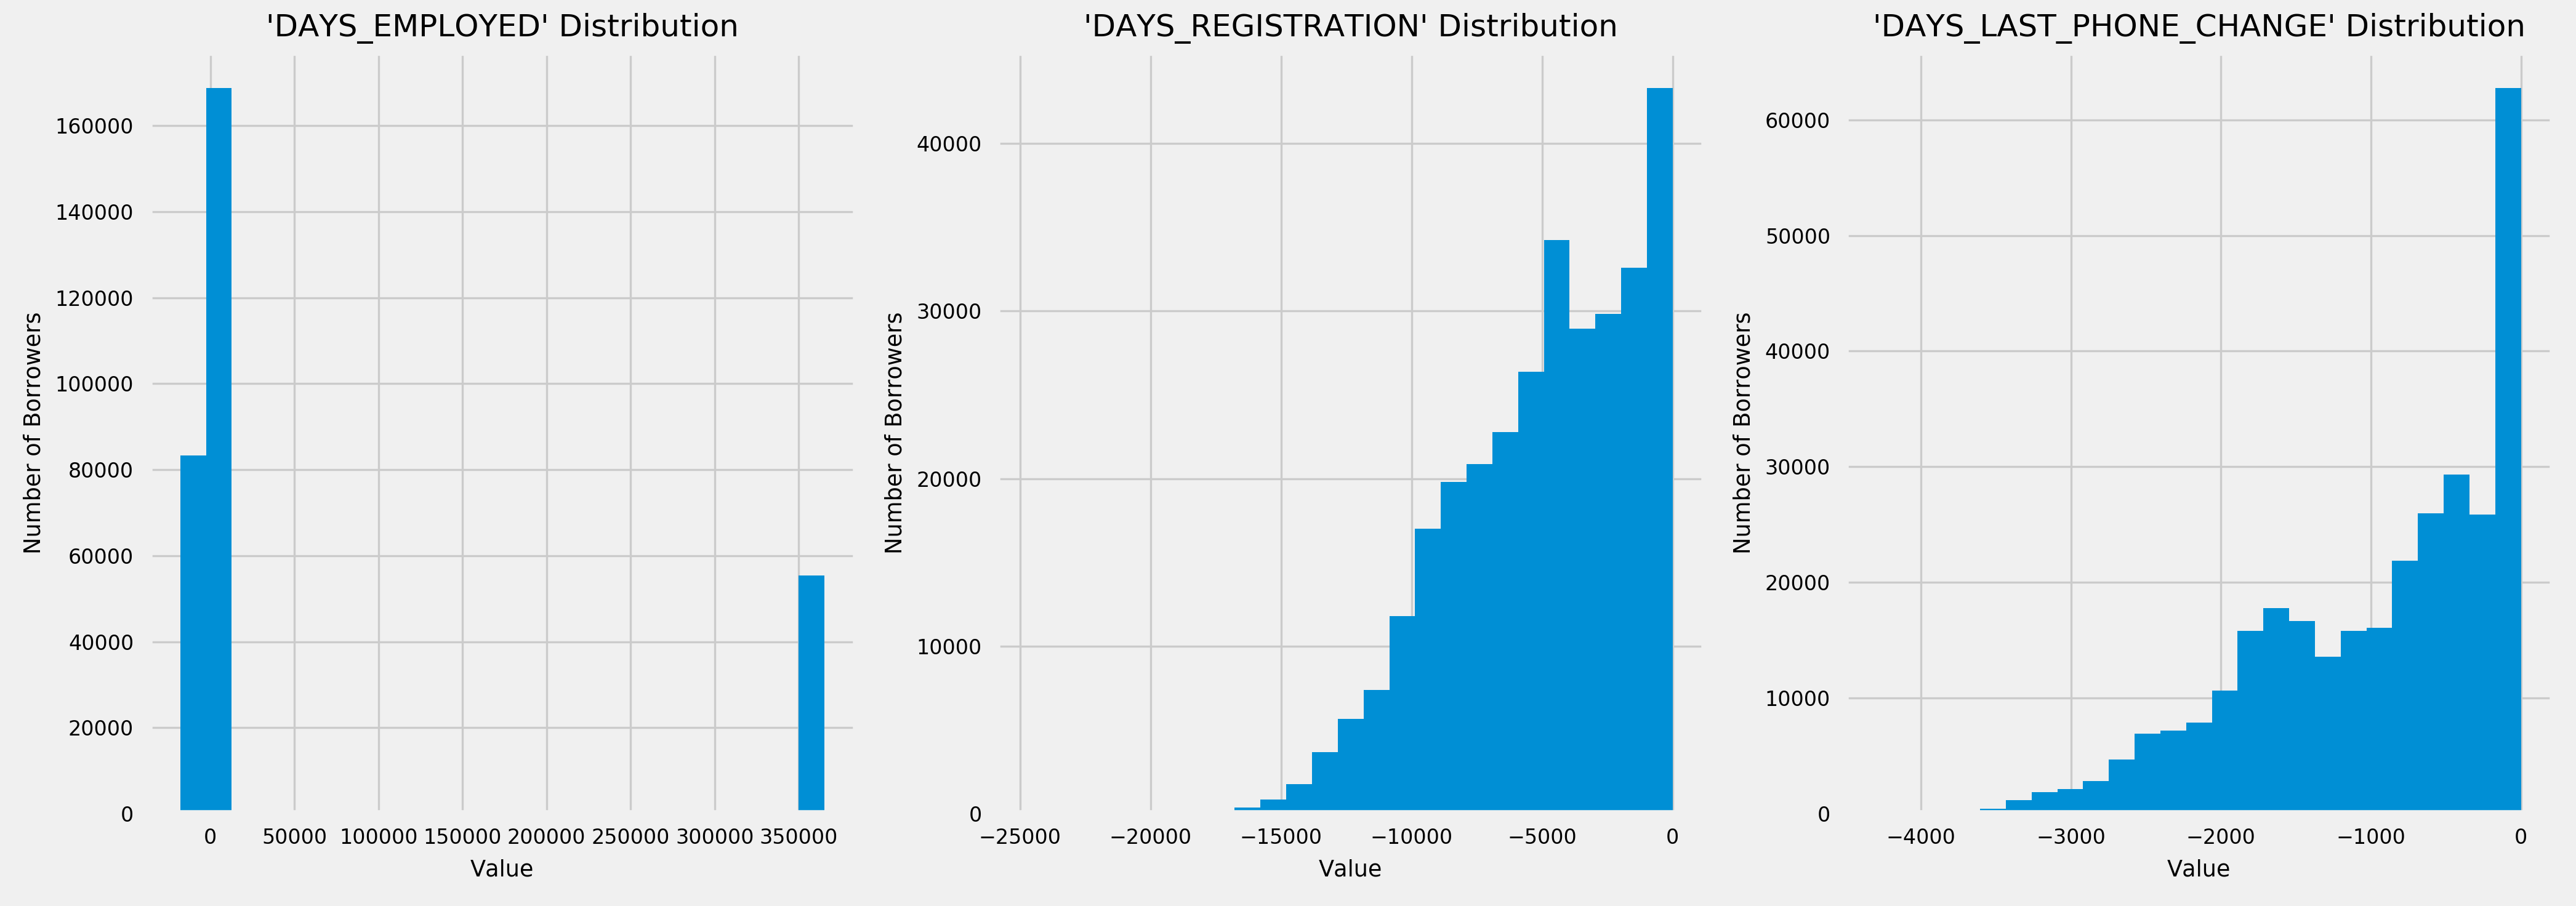
\includegraphics[width=\textwidth]{distribsDAYSEMPLOYEDDAYSREGISTRATIONDAYSLASTPHONECHANGE}
\centering
\caption{Distributions of Features \colorbox{backcolor}{\textcolor{black}{\texttt{DAYS_EMPLOYED}}}, \colorbox{backcolor}{\textcolor{black}{\texttt{DAYS_REGISTRATION}}}, \colorbox{backcolor}{\textcolor{black}{\texttt{DAYS_LAST_PHONE_CHANGE}}}}
\end{figure}

Finally, the two features \colorbox{backcolor}{\textcolor{black}{\texttt{DAYS_EMPLOYED}}} and \colorbox{backcolor}{\textcolor{black}{\texttt{OWN_CAR_AGE}}} contain an alarmingly large amount of high-valued outliers that will need to be addressed. I explore each of these features in depth below.

\subsubsection{Deeper Dive into the \colorbox{backcolor}{\textcolor{black}{\texttt{DAYS_EMPLOYED}}} Feature}
I observed that the \colorbox{backcolor}{\textcolor{black}{\texttt{DAYS_EMPLOYED}}} feature (the number of days before submitting their loan application that the applicant began their job) has more than 55,000 entries that contain impossibly large, positive entries similar to the value of 365,243 days (just over 1,000 years) that I had observed previously. The lone saving grace is that at least \colorbox{backcolor}{\textcolor{black}{\texttt{DAYS_EMPLOYED}}} has no `NaN' entries.

\begin{figure}[ht]
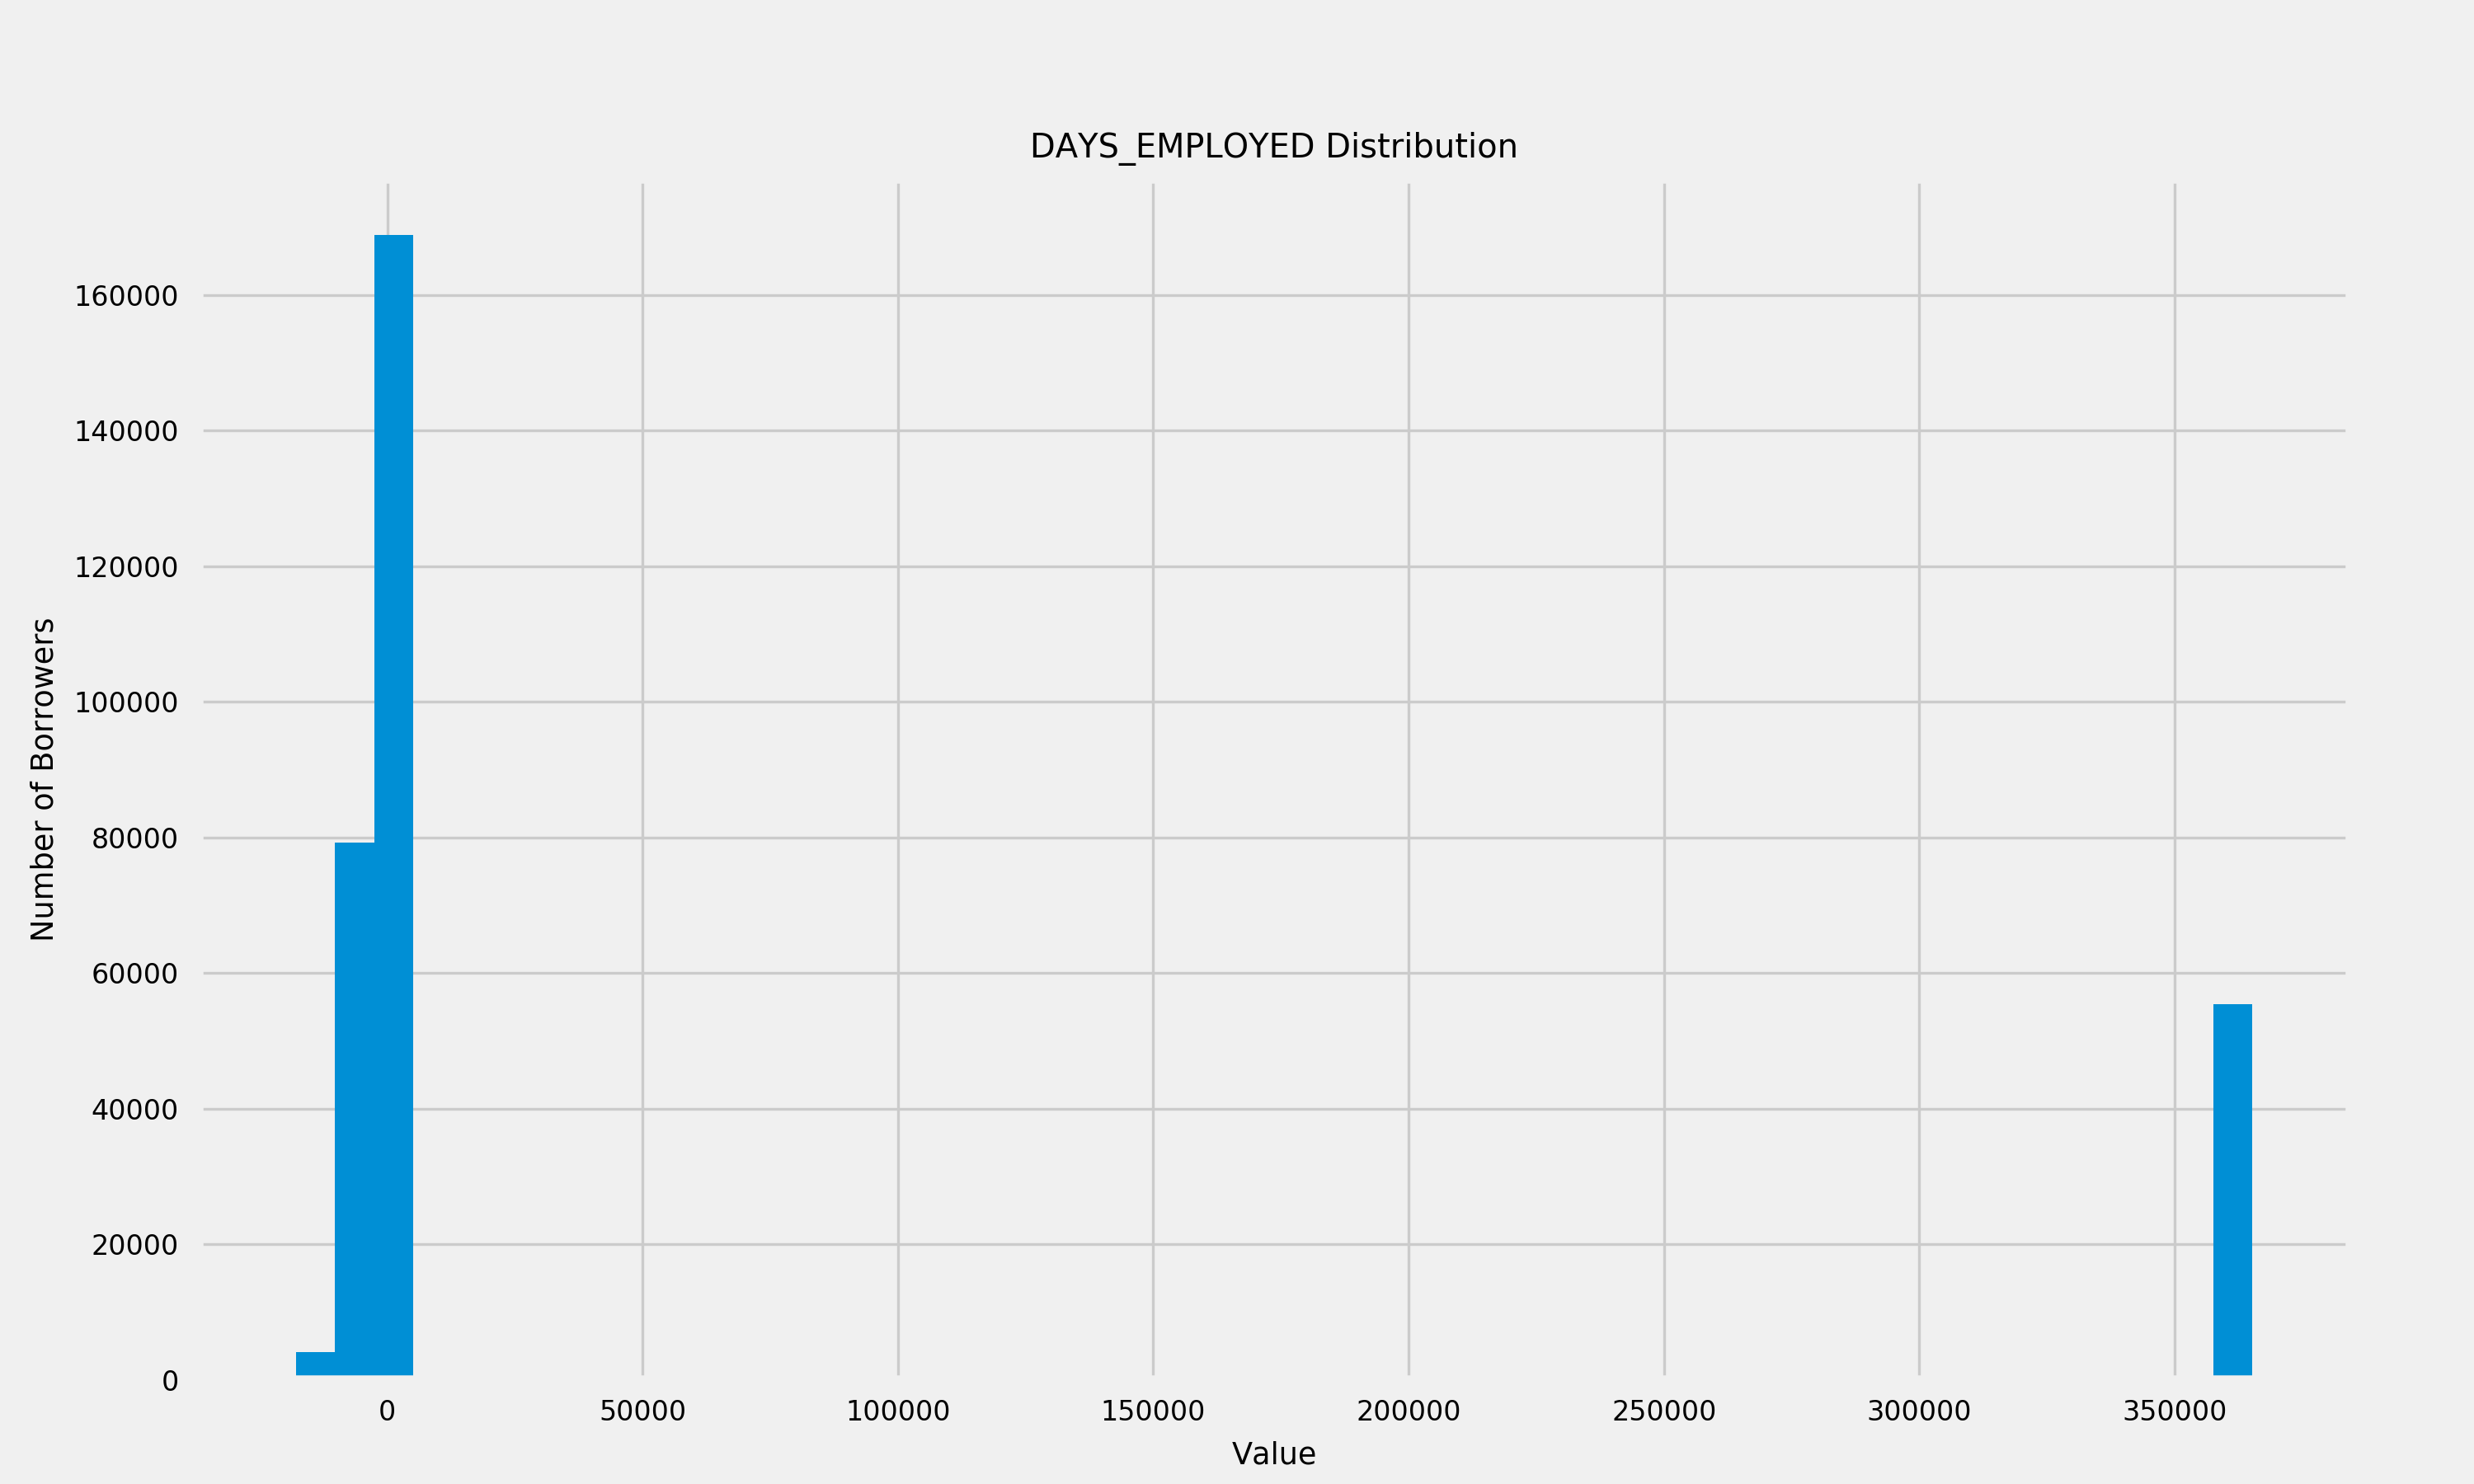
\includegraphics[width=0.7\textwidth]{distribDAYSEMPLOYED}
\centering
\caption{Distribution of Feature \colorbox{backcolor}{\textcolor{black}{\texttt{DAYS_EMPLOYED}}}}
\end{figure}

I ranked each value of \colorbox{backcolor}{\textcolor{black}{\texttt{DAYS_EMPLOYED}}} in descending order of frequency and confirmed that all these outlier entries had the same value of 365,243.

\begin{lstlisting}
 VALUE | COUNT
---------------
365243 |  55374
0      |      2
-1     |      1
-2     |      2
-3     |      3
-4     |      4
      ...
-17583 |      1
-17912 |      1
\end{lstlisting}

Based on the definition of \colorbox{backcolor}{\textcolor{black}{\texttt{DAYS_EMPLOYED}}}, valid values should be in the range ($\infty$,0]. Instead, exactly 55,374 entries, or nearly one-sixth of the entire training dataset, have entries of 365243. Were this to be interpreted literally, it would be an indication that one-sixth of the dataset got a job just over 1,000 years after submitting their loan applications to Home Credit.

This meaning is obviously absurd and there has to be another reason that so many borrowers had a value of 365243 for this feature. Since there were no instances of borrowers having different non-zero positive values, my best guess is that 365243 was not meant to indicate a numerical value. I believe that this value was entered into Home Credit's computer system when an applicant did not have a job when they submitted their loan application to Home Credit. Since any negative integer or 0 would be a valid entry under this feature, and perhaps due to the data entry system's inability to accept any datatype besides an integer, or perhaps due the system's inability to accept an empty (null) input in the feature's entry field, I hypothesize that the original data enterers at Home Credit simply entered the largest positive integer that the system would accept in order to indicate that the applicant didn't currently have a job.

Intuitively, I can see that all things being equal, \colorbox{backcolor}{\textcolor{black}{\texttt{DAYS_EMPLOYED}}} may well be a good predictor of target values. After all, if someone doesn't have a job or only just recently got a job, it stands to reason that there is a greater chance they won't have enough money to make loan payments on time. Unfortunately, I am not confident that the feature, as currently structured, will be able to adequately convey this information to a learning algorithm.

I therefore propose to replace the \colorbox{backcolor}{\textcolor{black}{\texttt{DAYS_EMPLOYED}}} feature with a new categorical feature called \colorbox{backcolor}{\textcolor{black}{\texttt{HAS_JOB}}}. All individuals who have a value of 365243 for \colorbox{backcolor}{\textcolor{black}{\texttt{DAYS_EMPLOYED}}} will be assigned a value of 0 for \colorbox{backcolor}{\textcolor{black}{\texttt{HAS_JOB}}}. All individuals who have a value of 0 or less for \colorbox{backcolor}{\textcolor{black}{\texttt{DAYS_EMPLOYED}}} will be assigned a value of 1 for \colorbox{backcolor}{\textcolor{black}{\texttt{HAS_JOB}}}.

\subsubsection{Deeper Dive into the \colorbox{backcolor}{\textcolor{black}{\texttt{OWN_CAR_AGE}}} Feature}
There appear to be just under 4,000 borrowers who have a value for \colorbox{backcolor}{\textcolor{black}{\texttt{OWN_CAR_AGE}}} that's between 60.0 and 70.0. This is far too many people than would be expected based on this feature's distribution.

\begin{figure}[ht]
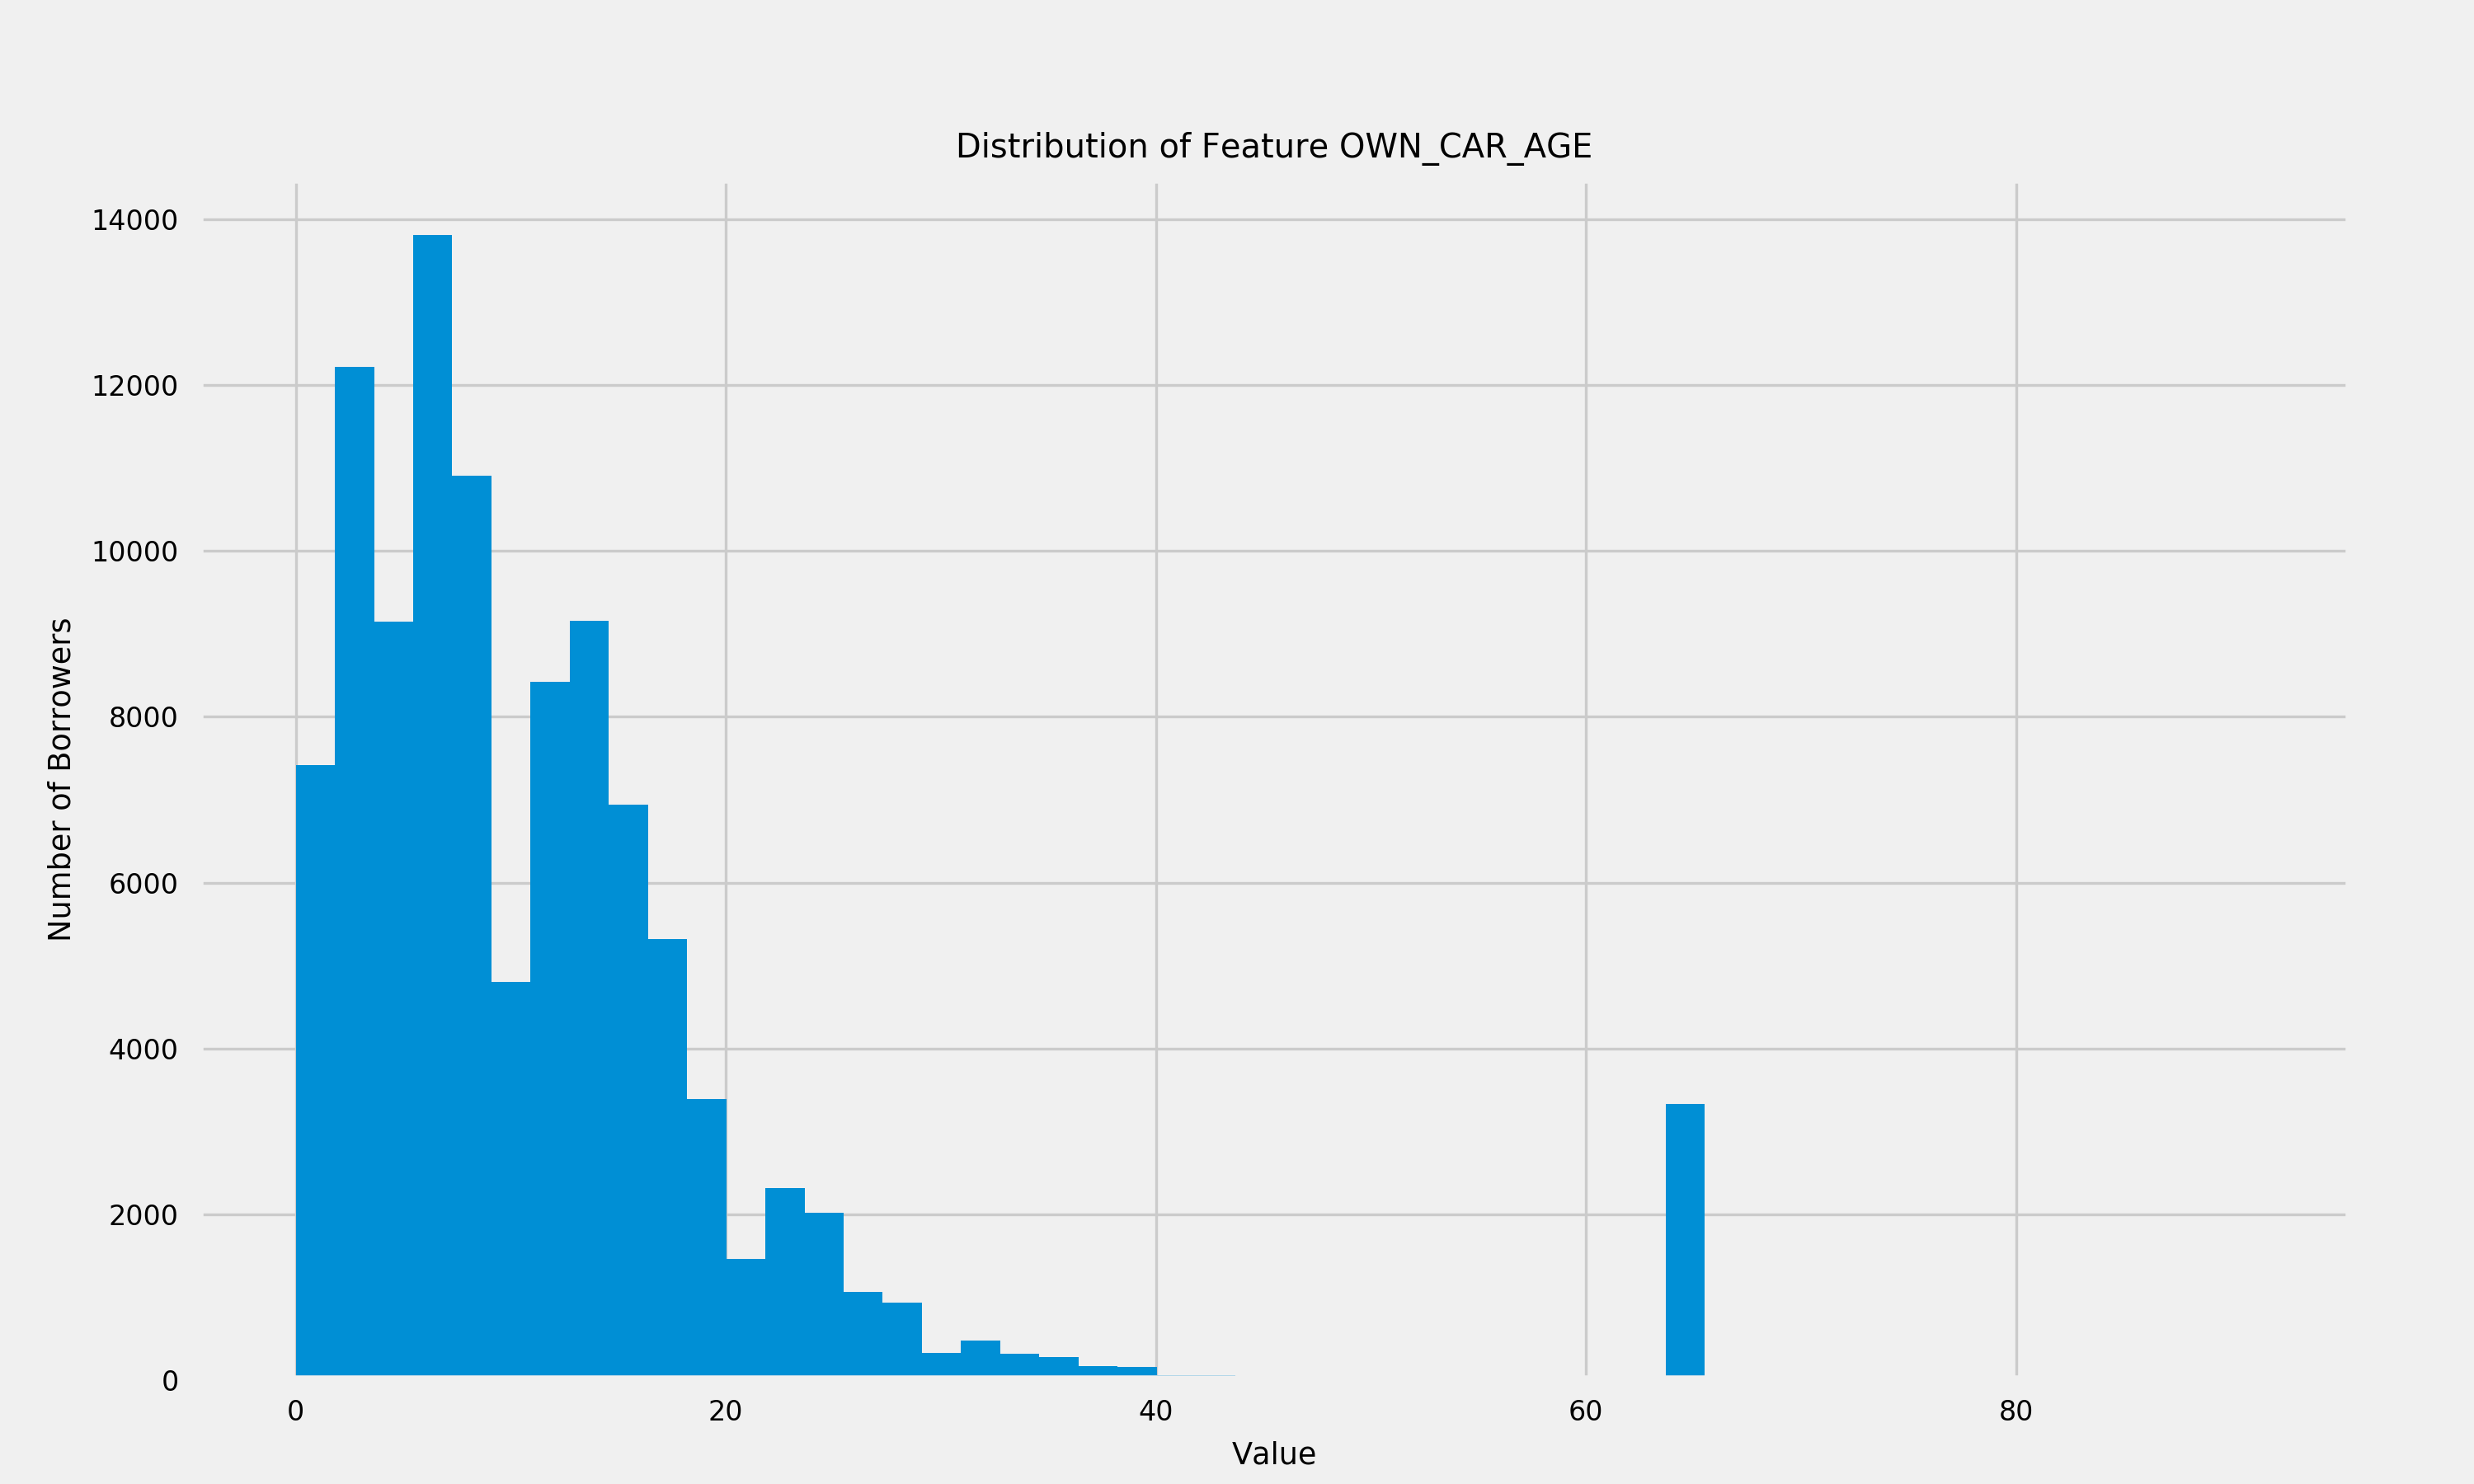
\includegraphics[width=0.7\textwidth]{distribOWNCARAGE}
\centering
\caption{Distribution of Feature \colorbox{backcolor}{\textcolor{black}{\texttt{OWN_CAR_AGE}}}}
\end{figure}

Specifically, there are 3,334 borrowers that have a car that's 64 or 65 years old.

\begin{lstlisting}
VALUE  |  COUNT
----------------
91.0   |      2
69.0   |      1
65.0   |    891
64.0   |   2443
63.0   |      2
57.0   |      1
56.0   |      1
      ...
2.0    |   5852
1.0    |   5280
0.0    |   2134
\end{lstlisting}

I can only conclude that this is evidence of some sort of anomaly -- I can think of no alternative logical explanation that could explain this spike. The only kinds of cars that are still functional after 60+ years are collectible classic cars, and folks who apply for loans from Home Credit come from a far less well-off demographic than that which is typically associated with classic car collecting.

Thankfully, I can see right away that the distribution of \colorbox{backcolor}{\textcolor{black}{\texttt{OWN_CAR_AGE}}} is less problematic than was the case for \colorbox{backcolor}{\textcolor{black}{\texttt{DAYS_EMPLOYED}}}. There is at least a smooth decrease in the frequency of users having older cars right up to the point where the anomalous spike occurs.

The distribution's pattern indicates that I should expect only one or two borrowers to have cars that are 64 or 65 years old, and yet I can't formulate a compelling justification for removing the outlier entries from the \colorbox{backcolor}{\textcolor{black}{\texttt{OWN_CAR_AGE}}} feature. Should all 3,334 of the datapoints in question be removed? Should all but a handful of them be removed? Indeed, doing this would keep the distribution smooth, but how would I choose which lucky few datapoints are kept in order to ensure the distribution is smooth over car ages of 64.0 and 65.0?

The good news is that I probably won't have to worry about this. Since 3,334 borrowers is only just over 3\% of the \colorbox{backcolor}{\textcolor{black}{\texttt{OWN_CAR_AGE}}} feature's 104,582 valid non-`NaN' entries, log-normalizing this feature should be enough to counteract any negative effects that the anomalous spike may have on a learning algorithm.

\subsection{Algorithms and Techniques}
Below I detail and justify the various algorithms and techniques that I implement at each of the three stages of my problem solving process.

\subsubsection{Data Preprocessing}
\begin{enumerate}
  \item \textbf{Create a cross-validation set that's 20\% of the size of the training data set}. Having a validation test set is necessary for model selection and for ensuring that trained learning algorithms are robust to overfitting and will generalize well to unseen data. In Kaggle competitions, it can be tempting to use the public leaderboard results during the competition to guage a model's performance. This is a huge mistake. Public leaderboard results are typically based on models' predictions on \textit{only} 20\% of the testing data table, or just 9,479 of the testing set's 48,744 rows or borrowers. There is no guarantee that these 9,479 rows are an adequate representation of the entire testing set, and thus there is no guarantee that a high score on the public leaderboard will translate to a high score at the end of the competition when final scores are based on the entire testing set.

  Using 20\% of the training data table, or 61,503 rows, as a test validation set enables me to gauge my models' performance in a way that is likely far more predictive of how they will perform on the entire testing set of 48,744 rows. One downside is that when comparing my various models against each other to see which is best, I can only train each model on 246,008 rows, as opposed to the full training set of 307,511 rows. A common workaround to this is to use an algorithm like K-Fold cross-validation, which allows models to be trained on every point in the training set before being compared to each other.

  However, due to the relatively large size of this training set, as well as due to the fact that I did not want to spend the extra time/money necessary to repeatedly run the more computationally expensive K-Fold cross validation algorithm, I decided that creating a simple train-test cross-validation split of the training dataset would suffice for this project.
  \item \textbf{Translate negative-valued features to positive ranges}. The two non-normalized features \colorbox{backcolor}{\textcolor{black}{\texttt{DAYS_REGISTRATION}}} and \colorbox{backcolor}{\textcolor{black}{\texttt{DAYS_LAST_PHONE_CHANGE}}} have significantly skewed distributions which will need to be log-normalized. However, since the log-normalization algorithm can only transform data that's distrbuted over positive ranges, each of these features' completely negative value ranges will be translated to the right such that the previously most-negative value of each distribution will become 0, and the new maximum value will be 0 plus the absolute value of that previously most-negative value.
  \item \textbf{Log-transform numerical features with skewed distributions}. Log-normalization may prevent the wide gulfs between these skewed features' very large and very small values from hindering a learning algorithm's performance.
  \item \textbf{Impute missing `NaN' values of all numerical features with each feature's mean}. Learning algorithms typically can't handle features that have missing entries. And since virtually all this dataset's numerical features contain one or more `NaN' entries, the only way to still use these features is to replace their missing values with a number. An imputer algorithm calculates a statistical measure, such as mean, of the valid numerical entries of a feature and then replaces each missing entry with that measure. There is always the risk that if too much of a feature's distribution is comprised of imputed numbers, that the feature may not be useful to learning algorithms. Nonetheless, since nearly all this dataset's numerical features have missing values, I believe I have no other choice but to impute the missing values and first make the attempt to use these features. I can always reduce or remove any unhelpful features during this project's refinement phase.
  \item \textbf{One-hot encode all categorical non-binary features}. At the end of the day, learning algorithms can only learn from features whose values are integer or float numbers. Unfortunately, many datasets have features such as gender or job type whose entries merely indicate categories like ``male" or ``accountant." The most direct way to transform this categorical data into numbers is to transform each one of these multi-categorical features into several individual binary features. For example, a categorical gender feature usually becomes two or more individual binary categorical features: gender-is-male, gender-is-female, etc. All individuals who had a category of ``male" for the original gender feature would now have an integer value of 1 for the new gender-is-male feature. All other individuals would have an integer value of 0 for this feature. The dataset's full featureset will ultimately contain 184 binary categorical features after one-hot encoding is complete.
  \item \textbf{Replace missing `NaN' values of one-hot encoded features with 0}. The case for doing this is even stronger than the case for imputing numerical features' missing entries with their means. If an individual has `NaN' for a binary categorical feature, it is reasonable to assume that that individual simply didn't belong to the category. Although this obviously can't be proven, it is the only possible logical inference that can be made in these cases. The alternative would be to throw out the entire feature, which I am not willing to do -- I believe that the knowledge of which individuals \textit{actually} had a value of 1 for a binary categorical feature, however sparse these folks may be, is valuable enough to justify making the assumption that all other folks with missing values didn't belong to the category to begin with.
  \item \textbf{Scale each numerical feature to the range [0,1]}. Most learning algorithms are designed with the assumption that all features vary on similar scales. Although tree-based estimators are robust to this assumption, any other estimators I might use, such as gradient-based estimators, would likely require this prerequisite. Furthermore, since the majority of the dataset's numerical features were already in the scale [0,1], I decided that for consistency's sake I would use a min-max scaling algorithm to scale the remaining numerical features to this range as well.
\end{enumerate}

\subsubsection{Implementation}
\begin{enumerate}
  \item \textbf{Gaussian Naive Bayes classifier}. I felt that a Naive Bayes classifier would be a greate algorithm to serve as a baseline benchmark right out of the box. It's quick to run, requires no hyperparameter tuning, and is robust to large featurespaces. It's also designed to be good at binary classification, which is goal of this project. Finally, Naive Bayes is able to output posterior probabilities of each of its Target predictions, which is something that any learning algorithm I use in this project must be able to do -- these actual proabilities are what will be submitted to Kaggle inside a CSV file.
  \item \textbf{AdaBoost classifier using a Decision Tree classifier as a base estimator}. AdaBoost is an adaptive learning algorithm, which means that it first fits a classifier (a Decision Tree classifier in this case) to the dataset, and then repeatedly fits additional copies of the same classifier on the dataset. However, on each iteration Adaboost adjusts the estimator's weights such that the next classifier focuses more on correctly classifying instances that were incorrectly classified by classifiers on prior iterations. This process of iteratively training classifiers, making predictions, and then adapting estimator weights is why AdaBoost is called a ``boosting" algorithm. Over several iterations, AdaBoost pays less attention to features that don't improve the model's predictive power, and focuses only on those features that do increase predictive power. It is largely because of this that I chose to use AdaBoost. I was concerned that a plain Decision Tree classifier might be at risk of overfitting to all 251 features that are in my data's unreduced featurespace. AdaBoost will allow me to observe how well a Decision Tree algorithm makes predictions, while guarding against the overfitting that might otherwise be a risk due to the large featurespace of my dataset.
  \item \textbf{GridSearchCV}. GridSearchCV is useful for automatially tuning hyperparameters. Although it can be more straightforward, and less computationally expensive, to manually tune a classifier's hyperparameters one parameter at a time, this can sometimes lead to an algorithm getting stuck at a local performance maxima. Indeed, there are situations where one particular \textit{combination} of hyperparameter values may be superior to a different \textit{combination}, but the chances of discovering the superior combination by adjusting one parameter at a time could be very remote. GridSearchCV generates a grid of hyperparameter combinations after the user specifies ranges of discrete values for each hyperparameter that they wish to tune. GridSearchCV then methodically trains a given classifier using each unique combination of hyperparameter values, and uses K-Fold cross validation and a scoring function specified by the user to compare the hyperparameter combinations and return the combination belonging to the classifier that scored highest. I will use GridSearchCV with AdaBoost in order to find an ideal tradeoff between AdaBoost's learning_rate and n_estimators parameters.

  Unfortunately GridSearchCV can be computationally expensive to run if there are several hyperparameters that can be tuned. This is all the more true when hyperparameters have large ranges of possible values. Therefore, in the interest of time, and because I intend to run my kernel locally on my laptop, I do not intend to use GridSearchCV with all learning algorithms I attempt to train.
  \item \textbf{Logistic Regression classifier}. Since logistic regression is often used for binary classification problems, it was one of the first learning algorithms I thought to use to solve this competition's goal of classifying borrowers into the two segments of delinquent repayers (Target = 1) and on-time repayers (Target = 0). Logistic regression generates coefficients for each of a dataset's features, and then constructs a linear equation composed of these features and their coefficients that can generate the best possible predictions of Target values for the majority of the dataset's datapoints (borrowers, in this case). As the logistic regression classifier gets trained on each point in the dataset, the value of each feature's coefficient is continually modified so as to maximize the likelihood of observing the sample values. Specifically, logistical regression adjusts the feature coefficients to maximize the logged odds of observing the sample values, or $ln(\frac{p}{1-p})$, where p is the probability that the user is a delinquent repayer if their observed Target value is 1, or the probability that they are an on-time repayer if their observed Target value is 0.

  A downside of logistic regression is that it assumes all features are independent. I will try my best to ensure that this will be the case for my dataset (ie. when re-engineering an existing feature, I will only keep the new, transformed feature and will discard the original feature that it was based on). However, given the size of the dataset's featurespace (it will have 251 features after one-hot encoding), the uncertain provenance of certain features, as well as my uncertainty about Home Credit's data entry methodology, it is not realistic for me to assume perfect independence among the featurespace's 251 features. Nonetheless, I am optimistic that my data will be robust enough such that logisitic regression will still work adequately at the very least.
  \item \textbf{Multi-Layer Perceptron classifier}. Multi-layer perceptron classifiers build a neural network comprised of several hidden layers that outputs a set of probability predictions for each point in the dataset. The predictions contain the probabilities that a point, or borrower in our case, belongs to each of the dataset's Target categories. Multi-layer perceptron classifiers can learn non-linear models, and can support a variety of activation functions, such as `relu' or `tanh', for generating probability predictions. I wanted to use a multi-layer perceptron simply to see how its performance compared to that of a linear logistic regression classifier when trained on this dataset. MLPs are sensitive to feature scaling and this is yet another reason I had to ensure that all my numerical features were scaled to the range [0,1].
  \item \textbf{LightGBM classifier}. For my final classifier, I wanted to use one of the two most widely used learning algorithms as of late, namely XGBOOST or LightGBM (gradient boosting machine). Similar to AdaBoost, XGBOOST and LightGBM are also boosting algorithms that are based on the decision tree algorithm. The difference between LightGBM and XGBOOST (and most other decision tree algorithms) is that LightGBM grows trees leaf-wise, instead of level-wise.

  \begin{figure}[ht]
  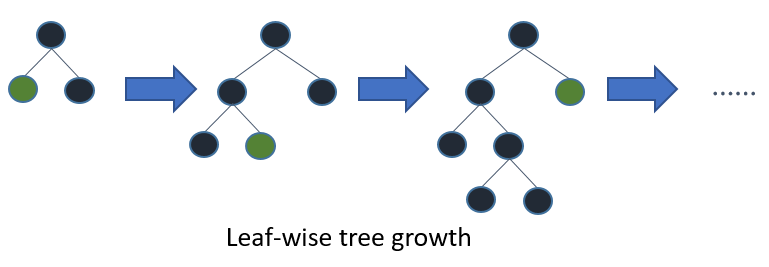
\includegraphics[width=0.7\textwidth]{leaf-wise}
  \centering
  \caption{Leaf-wise (Best-first) tree growth (LightGBM)\cite{lightgbmdocs}}
  \end{figure}

  \begin{figure}[ht]
  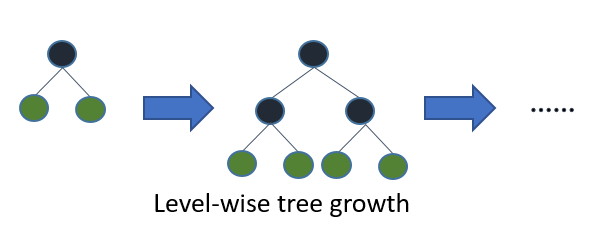
\includegraphics[width=0.7\textwidth]{level-wise}
  \centering
  \caption{Level-wise tree growth (XGBOOST and other decision tree algorithms)\cite{lightgbmdocs}}
  \end{figure}

  Growing trees leaf-wise can reduce more loss than growing trees level-wise, and LightGBM is therefore able to achieve better accuracy than many of the other boosting algorithms \cite{vidhyalightgbm}.

  Like XGBOOST, LightGBM is good with large datasets. However, LightGBM typically trains much faster than XGBOOST and also uses less memory. This final criteria is very important to me as during this project, I intend to create a kernel that can be run on my own laptop locally, without having to rent time on an Amazon EC2 instance.

  The main weak point of LightGBM is that the increased accuracy made possible by its leaf-wise splitting approach also raises the chance that the model will overfit to the training data.

  There are hyperparameters that can be tuned to prevent this, but this unfortunately leads to another downside of LightGBM, which is that it has \textit{a lot} of hyperparameters that can be tuned -- there are likely far more combinations than I can efficiently tune using an automatic algorithm like GridSearchCV locally on my laptop. However, one saving grace is that many of these hyperparameters merely offer different approaches to reaching the same goal, which is to take advantage of LightGBM's comparatively better accuracy without succumbing to overfitting.
\end{enumerate}

\subsubsection{Refinement}
\begin{enumerate}
  \item \textbf{PCA}. I will experiment with using Principle Component Analysis to reduce the dimensionality of my dataset's 67 numerical features. My approach will be to fit a PCA algorithm to the numerical features in the training dataset, and observe which and how many reduced components, or eigenvectors, explain the biggest chunks of roughly 90\% of the 67-dimension numerical featurespace's variance. I will then merge these PCA-reduced features back to the 184 binary features that are in the dataset after one-hot encoding, and re-train the above five learning algorithms on this reduced dataset.

  My hypothesis is that reducing the dimensionality of numerical features may help the performance of my learning algorithms, particularly logistic regression, that expect all training features to be independent. PCA works by finding a lower dimensional subspace on which to project a featurespace's higher dimensional features. The benefit is that redundant information in certain features that is correlated with other features' data is eliminated, all while only slightly raising the likelihood of added error. A reduced numerical featurespace may also benefit algorithms like LightGBM that have great accuracy but can be prone toward overfitting.

  Of course, this approach could backfire if it turns out that there are a small amount of numerical features that in their raw, unreduced form are more useful to my learning algorithms than any of the reduced components produced by PCA.
  \item \textbf{SelectKBest}. Applying PCA can mitigate against noise and correlation amongst my featureset's 67 numerical features, but what about the 184 categorical features that will exist after one-hot encoding is complete? I want to investigate whether reducing the scope of the entire featureset, not just numerical features, will possibly help sharpen the focus of my learning algorithms, and enable them to make predictions that generalize better to unseen data.

  A common technique for this kind of feature selection is to use the algorithm SelectKBest. SelectKBest computes a score for each feature in a dataset and then modifies the dataset, removing all but the top K scoring features. Several kinds of scoring functions can be used. I will use the f_classif scoring function, which computes the ANOVA F-value between a feature and a label. This type of scoring function is useful for measuring how well a feature contributes to classification tasks, which is precisely what this competition is.

  There is no clear rule of thumb for determining the ideal K number of a dataset's features to keep. I plan to try a few different values of K, and see if I can find a value that results in improved performance in any of the above five learning algorithms when they are trained on those K features.
\end{enumerate}

\subsection{Benchmark}
Solutions to this competition will be ranked on Kaggle by the area under the ROC curve between their predicted proabilities and the observed targets (whether or not the borrower was actually delinquent).

I will train a Gaussian Naive Bayes classifier on a fully preprocessed dataset and use its ROC area under curve score as my primary benchmark. Gaussian Naive Bayes is ideal for this because it needs no hyperparameter input nor tuning. It also trains faster than most other models and I should have no difficulty training it on the dataset's 300,000+ rows locally on my own machine. I am optimistic that with appropriate model selection and hyperparameter tuning I will be able to build a learning algorithm that outperforms this simple out-of-the-box Gaussian Naive Bayes model.

In order to guage how my solution compares to others in the Kaggle community, I will use the average ROC curve area of all entries on the competition's public leaderboard\cite{kagglehomecreditcompetitionpublicleaderboard} as of June 2, 2018 as a secondary, personal benchmark. As of this date, there were 5,398 total entries from 1,515 participants. The average area under the ROC curves of all entries was \colorbox{backcolor}{\textcolor{red}{\texttt{0.7379}}}. I hope to design an algorithm that will meet or exceed this score. The reader may refer to the file \colorbox{backcolor}{\textcolor{black}{\texttt{home-credit-default-risk-publicleaderboard(6-02-2018).csv}}}, located inside this project's Github repository\cite{githubprojectrepo}, to verify my calculation of this secondary benchmark.

It would also be nice to know the area under ROC curve of the prediction model employed by Home Credit's data scientists prior to this competition's debut on Kaggle. However, since Home Credit possibly considers this model and its ROC curve area to be proprietary information, it is understandable that it was not disclosed.

\section{Methodology}
\subsection{Data Preprocessing}
I proceeded through the following 19 steps when preprocessing my dataset.

\begin{enumerate}
 \item Create 7 lists that categorize the dataset's features into following groups based on how each feature will need to be preprocessed:
   \begin{enumerate}
    \item Categorical features needing one-hot encoding
    \item Binary categorical features
    \item Non-normalized numerical features with skewed distributions and negative values
    \item Non-normalized numerical features with skewed distributions and only positive values
    \item Numerical features with normal distributions, but not scaled to the range [0,1]
    \item Numerical features with normal distributions and scaled to the range [0,1]
    \item Features that will be re-engineered and transformed into different features
  \end{enumerate}
  Creating these 7 lists keeps my preprocessing organized, and allows me to quickly slice the datatable to access only the features that will need to be adjusted during a particular preprocessing step.
  \item Separate the Targets column out from training dataset.
  \item Use train_test_split from sklearn.cross_validation to create a test validation set that is 20\% of the size of the total training set.
  \item Use the numerical \colorbox{backcolor}{\textcolor{black}{\texttt{CNT_CHILDREN}}} feature to engineer a binary categorical feature called \colorbox{backcolor}{\textcolor{black}{\texttt{HAS_CHILDREN}}}. The value of \colorbox{backcolor}{\textcolor{black}{\texttt{HAS_CHILDREN}}} will be 1 if the borrower has one or more children, otherwise the value will be 0.
  \item Drop the \colorbox{backcolor}{\textcolor{black}{\texttt{CNT_CHILDREN}}} feature from the main dataframe. This is done to keep the features as independent as possible.
  \item Use the \colorbox{backcolor}{\textcolor{black}{\texttt{CNT_FAM_MEMBERS}}} feature to engineer a categorical feature called \colorbox{backcolor}{\textcolor{black}{\texttt{FAMILY_SIZE}}}. \colorbox{backcolor}{\textcolor{black}{\texttt{FAMILY_SIZE}}} will be a multi-categorical feature that will be one-hot encoded along with the other 18 non-binary categorical features that were originally included in the dataset. \colorbox{backcolor}{\textcolor{black}{\texttt{FAMILY_SIZE}}} will have the values of ``one," ``two," or ``three_plus" depending on the numerical value of \colorbox{backcolor}{\textcolor{black}{\texttt{FAMILY_SIZE}}}.
  \item Drop \colorbox{backcolor}{\textcolor{black}{\texttt{CNT_FAM_MEMBERS}}} from the main dataframe.
  \item Use the \colorbox{backcolor}{\textcolor{black}{\texttt{CREDIT_DAY_OVERDUE}}} feature in \colorbox{backcolor}{\textcolor{black}{\texttt{bureau.csv}}} to engineer the binary categorical \colorbox{backcolor}{\textcolor{black}{\texttt{HAS_CREDIT_BUREAU_LOANS_OVERDUE}}} feature. The value for \colorbox{backcolor}{\textcolor{black}{\texttt{HAS_CREDIT_BUREAU_LOANS_OVERDUE}}} will be 1 if the borrower has at least one loan in \colorbox{backcolor}{\textcolor{black}{\texttt{bureau.csv}}} that has a value for \colorbox{backcolor}{\textcolor{black}{\texttt{CREDIT_DAY_OVERDUE}}} that's greater than zero, and 0 otherwise.
  \item Use the \colorbox{backcolor}{\textcolor{black}{\texttt{DAYS_EMPLOYED}}} feature to engineer a binary categorical feature called \colorbox{backcolor}{\textcolor{black}{\texttt{HAS_JOB}}}. If a borrower has a negative value or zero for \colorbox{backcolor}{\textcolor{black}{\texttt{DAYS_EMPLOYED}}}, then \colorbox{backcolor}{\textcolor{black}{\texttt{HAS_JOB}}} will be 1, otherwise \colorbox{backcolor}{\textcolor{black}{\texttt{HAS_JOB}}} will be 0.
  \item Drop the \colorbox{backcolor}{\textcolor{black}{\texttt{DAYS_EMPLOYED}}} feature from the main dataframe.
  \item Translate to positive ranges all values of the 2 remaining non-normalized numerical features that have skewed distributions and negative values: \colorbox{backcolor}{\textcolor{black}{\texttt{DAYS_REGISTRATION}}}, and \colorbox{backcolor}{\textcolor{black}{\texttt{DAYS_LAST_PHONE_CHANGE}}}.
  \item Log-transform all 17 non-normalized numerical features that have skewed distributions. These 17 features include the 2 that were translated to positive ranges in Step 11.
  \item Replace `NaN' values for all numerical features with each feature's mean using Sklearn's Imputer class.
  \item Remove the borrower ID column, \colorbox{backcolor}{\textcolor{black}{\texttt{SK_ID_CURR}}}, from the main dataframe.
  \item One-hot encode all 19 now non-binary categorical features.
  \item Replace all `NaN' values in all binary categorical features with 0.
  \item Fit a min-max scaler to each of the 17 log-transformed numerical features, as well as to the features \colorbox{backcolor}{\textcolor{black}{\texttt{DAYS_BIRTH}}}, \colorbox{backcolor}{\textcolor{black}{\texttt{DAYS_ID_PUBLISH}}}, \colorbox{backcolor}{\textcolor{black}{\texttt{HOUR_APPR_PROCESS_START}}}, and the normalized feature \colorbox{backcolor}{\textcolor{black}{\texttt{REGION_POPULATION_RELATIVE}}}. Each feature will be scaled to a range [0.0, 1.0].
  \item Build a data preprocessing pipeline to used to preprocess both the test validation and actual testing sets. This pipeline will:
  \begin{enumerate}
    \item Recreate all features that were engineered in the training set during the original data preprocessing phase.
    \item Impute missing numerical values with each column's mean.
    \item Replace missing `NaN' values of binary categorical features with 0. \item Apply the min-max scaling transforms originally fit on features in the training set to all data points in a testing set.
    \item Finally, any columns representing binary one-hot encoded features that are in the training set but absent from a test set will be added to the test set and filled with all 0s. Similarly, any columns in a test dataframe that represent one-hot encoded features that aren't present in the training set will be removed from the test dataframe. We always change the test set's columns to ensure they are consistent with those of the training set, not the other way around. This ensures that the final model is as robust as possible to unseen data.

    This kind of adjustment will be necessary when making predictions on the testing datatable in \colorbox{backcolor}{\textcolor{black}{\texttt{application_test.csv}}}, which after one-hot encoding will have one column not in the training set, and will be missing two columns that are in the training set.

    This sort of phenomenon sometimes arises after one-hot encoding. When a multi-categorical feature has some rows in one datatable that have a certain category value, while the corresponding feature in another data table has no rows that have that category value, the two datatables will not have identical sets of binary features after one-hot encoding.
  \end{enumerate}
  \item Use the preprocessing pipeline built in Step 18 to preprocess the test validation set.
\end{enumerate}

\subsection{Implementation}
I followed the steps below when implementing my learning algorithms, training them on the fully processed featureset of 251 features, and scoring their predictions on the test validation set.

\begin{enumerate}
  \item Create an ROC area-under-curve scorer method that uses Sklearn's roc_auc_score() method. This scoring function was used to compute the ROC AUC scores of each classifier's predictions on the validation set. It will also be wrapped in Sklearn's make_scorer() method to create a scoring object that can be used by GridSearchCV objects.
  \item Train a Gaussian Naive Bayes classifier on the training set and use it to make predictions on the test validation set. Calculate the area under ROC curve score of these predictions. No hyperparameters will be needed for this classifier.
  \item Use GridSearchCV to explore the tradeoff between values for the 'learning_rate' and 'n_estimators' hyperparameters for an AdaBoost classifier that uses a Decision Tree classifier as its base estimator, scoring each combination by ROC AUC score:
  \begin{lstlisting}
params = {
      'learning_rate': [0.01, 0.1, 1.0],
      'n_estimators': [200, 250, 500,1000],
      'random_state': [42]
  }
  \end{lstlisting}
  I discovered that the highest scoring AdaBoost classifier had learning_rate=1.0 and n_estimators=1000.
  \item I then made predictions on the validation set using this AdaBoost classifier and noted ther ROC AUC score.
  \item Train a Logistic Regression classifier, make predictions on the validation set, and compute the ROC AUC score.
  \item Train a Multi-Layer Perceptron classifier, make predictions on the validation set, and compute the ROC AUC score.
  \item Train a LightGBM classifier, make predictions on the validation set, and compute the ROC AUC score. Implenting LightGBM entails some unique steps not necessary when implementing the more run-of-the-mill classifiers included in Sklearn:
    \begin{enumerate}
      \item THe LightGBM package must be installed inside my Anaconda environment.
      \item The training data must be converted to the LightGBM dataset format before the classifier can be trained:
      \begin{lstlisting}
lightgbm_training =
lgb.Dataset(X_train_final, label=y_train)
      \end{lstlisting}
      \item Conveniently, LightGBM's predict() method outputs a list of probability predictions that can be directly entered into the roc_auc() method to compute the ROC AUC score. Other classifers output an array containing two columns, from which the second column must be sliced before being used to compute the ROC_AUC score, as is the case for the Multi-Layer Perceptron classifier's predictions:
      \begin{lstlisting}
mlp_y_score =
clf_mlp.predict_proba(X_test_final)[:, 1]
      \end{lstlisting}
    \end{enumerate}
  \end{enumerate}
  Note that for the Logistic Regression, Multi-Layer Perceptron, and LightGBM classifiers, I manually tuned hyperparameter values until I could no longer improve the classifiers' ROC AUC scores on the validation set. In the interest of time, I decided to hold off on using GridSearchCV again until I had identified highest performing classifier/featureset combination during the refinement phase. At that time I would perform one final round of hyperparameter tuning on the best performing classifier up to that point. As I trained and scored each classifier during the implementation phase, it became clear to me that I would be able to identify the most promising classifier without extensive tuning of each classifier's hyperparameters.

\subsection{Refinement}
Below are the ROC AUC scores of each classifier's predictions on the validation set, after each classifier has been trained on the full featureset of 251 features:

\begin{table}[ht]
  \centering
  \definecolor{lightgray}{gray}{0.92}
  {\rowcolors{2}{white}{lightgray}
  \begin{tabular}{|| l | l ||}
   \hline
   \multicolumn{2}{|c|}{All Features} \\
   \hline
   \rowcolor{white} \textbf{Classifier} & \textbf{ROC AUC Score} \\ [0.5ex]
   \hline\hline
   Naive Bayes & 0.546645662333944 \\
   \hline
   AdaBoost & 0.7462758964509755 \\
   \hline
   Logistic Regression & 0.7471756350178691 \\
   \hline
   Multi-layer Perceptron & 0.7429017839300756 \\
   \hline
   LightGBM & 0.7592132612569703 \\ [1ex]
   \hline
  \end{tabular}
 }
 \caption{Validation set prediction ROC AUC scores of classifiers trained on the full featureset.}
 \label{table:1}
\end{table}

It's immediately clear that LightGBM's performance is head and shoulders above the rest of the classifiers, with an ROC AUC score that's more than a full percentage point higher than that of the second best performing classifier, Logistic Regression. What's more, I observed that LightGBM could be trained in less time than most of the other classifiers, particularly AdaBoost.

I next wanted to see if reducing the dimensionality of the featureset's 67 numerical features would enable one of the above classifiers to surpass LightGBM's ROC AUC score of \colorbox{backcolor}{\textcolor{red}{\texttt{0.7592}}}. I followed these steps to apply PCA to the training and validation datasets :
\begin{enumerate}
  \item Fit PCA on all 67 numerical features, trying different values for the n_components parameter in order to determine how many principle components are needed to explain roughly 90\% of the variance in the numerical features.
  \item I discovered that 17 principle components will explain approximately 90\% of the variance in all the numerical features:
  \begin{lstlisting}
Explained variance ratios for each component:
[ 0.1712049   0.12231898  0.09857175  0.06724392
  0.05962164  0.05682911  0.05083881  0.04976384
  0.04510004  0.04230571  0.02981382  0.02512118
  0.01950228  0.01827228  0.01581516  0.0155643
  0.01255201]

90.04% of variance of numerical features
explained by 17 components.
  \end{lstlisting}
  \item I then fit a PCA algorithm (with n_components parameter set to 17) to all 67 numerical features in the training set, and used it to transform the training set's numerical features, reducinging them to just 17 features:
  \begin{lstlisting}
reduced_numerical_data =
pca.transform(X_train_processed[numerical_features])
  \end{lstlisting}
  \item I next created a dataframe to store these reduced features.
  \item Finally, I dropped all 67 numerical features from the original preprocessed training dataframe, so that it only contained the 184 binary categorical features. I then merged the dataframe containing the PCA-reduced numerical features back to this dataframe, resulting in a training set with 201 features.
  \item I also used the above PCA algorithm that had been fit on the training data to transform the validation set's 67 numerical features into their 17 PCA-reduced counterparts.
\end {enumerate}

I then trained my five classifier algorithms (with hyperparameters unchanged) on this PCA-reduced training set of 201 total features, and used them to make predictions on the validation set after it had also been processed to account for the PCA dimensionality reduction.

\begin{table}[ht]
  \centering
  \definecolor{lightgray}{gray}{0.92}
  {\rowcolors{2}{white}{lightgray}
  \begin{tabular}{|| l | l ||}
   \hline
   \multicolumn{2}{|c|}{PCA} \\
   \hline
   \rowcolor{white} \textbf{Classifier} & \textbf{ROC AUC Score} \\ [0.5ex]
   \hline\hline
   Naive Bayes & 0.5452255614331999 \\
   \hline
   AdaBoost & 0.7415669749755673 \\
   \hline
   Logistic Regression & 0.743963963781135 \\
   \hline
   Multi-layer Perceptron & 0.7439527449175637 \\
   \hline
   LightGBM & 0.7483887050110797 \\ [1ex]
   \hline
  \end{tabular}
 }
 \caption{Validation set prediction ROC AUC scores of classifiers trained on the 17 PCA-reduced numerical features and 184 binary features.}
 \label{table:2}
\end{table}

Unfortunately, other than the score of the Multi-Layer Perceptron, which had a slight improvement, all other classifiers' ROC AUC scores on the validation set dropped after using PCA to reduce the dimension space of the numerical features. Notably, my LightGBM classifier's score, although still better than those of all other classifiers, fell more than a full percentage point to \colorbox{backcolor}{\textcolor{red}{\texttt{0.7483}}}. I could only conclude that there must be certain numerical features that were more valuable to my learning algorithms in their unreduced, original dimensions.

I still wanted to test my final hypothesis, which was that a select group of features taken from the original 251 numerical and binary features would enable one or more of my learning algorithms to improve their ROC AUC scores on the validation set. I implemented SelectKBest with different values of K to see if there is a group of K features that results in improved performance of the learning algorithms when they are trained on just these K features.

\begin{table}[h!]
  \centering
  \definecolor{lightgray}{gray}{0.92}
  {\rowcolors{2}{white}{lightgray}
  \begin{tabular}{|| l | l ||}
   \hline
   \multicolumn{2}{|c|}{SelectKBest, K=20} \\
   \hline
   \rowcolor{white} \textbf{Classifier} & \textbf{ROC AUC Score} \\ [0.5ex]
   \hline\hline
   Naive Bayes & 0.6833259704479555 \\
   \hline
   AdaBoost & 0.7376556539610273 \\
   \hline
   Logistic Regression & 0.7353141520826144 \\
   \hline
   Multi-layer Perceptron & 0.7340542201102302 \\
   \hline
   LightGBM & 0.7347991347869498 \\ [1ex]
   \hline
  \end{tabular}
 }
 \caption{Validation set prediction ROC AUC scores of classifiers trained on the top 20 features chosen using SelectKBest, K=20.}
 \label{table:3}
\end{table}

\begin{table}[h!]
  \centering
  \definecolor{lightgray}{gray}{0.92}
  {\rowcolors{2}{white}{lightgray}
  \begin{tabular}{|| l | l ||}
   \hline
   \multicolumn{2}{|c|}{SelectKBest, K=30} \\
   \hline
   \rowcolor{white} \textbf{Classifier} & \textbf{ROC AUC Score} \\ [0.5ex]
   \hline\hline
   Naive Bayes & 0.6748662184461512 \\
   \hline
   AdaBoost & 0.7330739254581403 \\
   \hline
   Logistic Regression & 0.7367180213600446 \\
   \hline
   Multi-layer Perceptron & 0.7358901049573279 \\
   \hline
   LightGBM & 0.7394787228642934 \\ [1ex]
   \hline
  \end{tabular}
 }
 \caption{Validation set prediction ROC AUC scores of classifiers trained on the top 30 features chosen using SelectKBest, K=30.}
 \label{table:4}
\end{table}

\pagebreak

\begin{table}[h!]
  \centering
  \definecolor{lightgray}{gray}{0.92}
  {\rowcolors{2}{white}{lightgray}
  \begin{tabular}{|| l | l ||}
   \hline
   \multicolumn{2}{|c|}{SelectKBest, K=60} \\
   \hline
   \rowcolor{white} \textbf{Classifier} & \textbf{ROC AUC Score} \\ [0.5ex]
   \hline\hline
   Naive Bayes & 0.6684098231997853 \\
   \hline
   AdaBoost & 0.7438097973020747 \\
   \hline
   Logistic Regression & 0.7417987588406878 \\
   \hline
   Multi-layer Perceptron & 0.7403314315263486 \\
   \hline
   LightGBM & 0.7522811504663048 \\ [1ex]
   \hline
  \end{tabular}
 }
 \caption{Validation set prediction ROC AUC scores of classifiers trained on the top 60 features chosen using SelectKBest, K=60.}
 \label{table:5}
\end{table}

\begin{table}[h!]
  \centering
  \definecolor{lightgray}{gray}{0.92}
  {\rowcolors{2}{white}{lightgray}
  \begin{tabular}{|| l | l ||}
   \hline
   \multicolumn{2}{|c|}{SelectKBest, K=120} \\
   \hline
   \rowcolor{white} \textbf{Classifier} & \textbf{ROC AUC Score} \\ [0.5ex]
   \hline\hline
   Naive Bayes & 0.6522417061567687 \\
   \hline
   AdaBoost & 0.7477080344062966 \\
   \hline
   Logistic Regression & 0.7462061715711668 \\
   \hline
   Multi-layer Perceptron & 0.7422206488500489 \\
   \hline
   LightGBM & 0.7559874806914961 \\ [1ex]
   \hline
  \end{tabular}
 }
 \caption{Validation set prediction ROC AUC scores of classifiers trained on the top 120 features chosen using SelectKBest, K=120.}
 \label{table:6}
\end{table}

\begin{table}[h!]
  \centering
  \definecolor{lightgray}{gray}{0.92}
  {\rowcolors{2}{white}{lightgray}
  \begin{tabular}{|| l | l ||}
   \hline
   \multicolumn{2}{|c|}{SelectKBest, K=200} \\
   \hline
   \rowcolor{white} \textbf{Classifier} & \textbf{ROC AUC Score} \\ [0.5ex]
   \hline\hline
   Naive Bayes & 0.6368790945859744 \\
   \hline
   AdaBoost & 0.7498569541301328 \\
   \hline
   Logistic Regression & 0.74715371178638 \\
   \hline
   Multi-layer Perceptron & 0.7438126377468326 \\
   \hline
   LightGBM & 0.7581504347134562 \\ [1ex]
   \hline
  \end{tabular}
 }
 \caption{Validation set prediction ROC AUC scores of classifiers trained on the top 200 features chosen using SelectKBest, K=200.}
 \label{table:7}
\end{table}

Although the performance of the Naive Bayes classifier saw substantial improvement when the featurespace was reduced to K=20 features, its ROC AUC score was still much lower than those of the four other classifiers. And as for those four other classifiers, the trend here is unmistakable: these classifiers' ROC AUC scores dropped significantly when the featurespace was reduced to 20 features (LightGBM's score was \colorbox{backcolor}{\textcolor{red}{\texttt{0.7348}}}), and then steadily increased as the feature space was increased to K=30, 60, 120, and finally, 200 features. At K=200, LightGBM's score was \colorbox{backcolor}{\textcolor{red}{\texttt{0.7582}}}.

This was the clearest possible confirmation that my best performing learning algorithm, LightGBM, would perform at its best when trained on the full featurespace of 251 features. This combination had provided, so far, a top ROC AUC score of \colorbox{backcolor}{\textcolor{red}{\texttt{0.7592}}} on the validation set.

However, before using this classifier to compute predictions on the test set in order to submit to Kaggle, I wanted to first see if I could further optimize its hyperparameters using GridSearchCV.

I encountered a few unexpected hiccups when setting up GridSearchCV to tune a LightGBM classifier:
\begin{enumerate}
  \item It turned out that I needed to use the LGBMClassifier() class to initialize my LightGBM classifier and then directly specify its parameter values before passing the classifier itself as a parameter to GridSearchCV. (When training a standalone LightGBM classifier, I'd ordinarily only need to need to call LightGBM's train() method and pass it a single dictionary containing all the hyperparameter values.) For example:
  \begin{lstlisting}
# Create an LightGBM classifier object
clf = lgb.LGBMClassifier(boosting_type = 'gbdt',
                         objective = 'binary',
                         metric = 'auc')
  \end{lstlisting}
  \item I did not need to convert the dataset to LightGBM format prior to passing it to the GridSearchCV object's fit() method.
  \item Unlike plain LightGBM, whose predict() method returns a list
  of prediction probabilities that I can pass directly to Sklearn's roc_auc method to calculate the ROC AUC score, in order access the ROC AUC score of the LightGBM hyperparameter combination returned by GridSearchCV, I must call GridSearchCV's predict_proba() method, slice it to access the second column of the array that it returns, and then pass this list as a parameter to roc_auc:
  \begin{lstlisting}
roc_auc_score(y_test,grid.predict_proba(X_test_final)[:,1])
  \end{lstlisting}
  \item Finally, and most significantly, LightGBM has far too many hyperparameters than could be thoroughly investigated by running GridSearchCV locally on my laptop.
\end{enumerate}

My approach was thus to use GridSearchCV to investigate the interplay between LightGBM's num_iterations, num_leaves, and learning_rate hyperparameters, and to develop intuition about which combination of these parameters' values would work best with my data's full featureset. I found that having a num_iterations value of at least 10,000, with a learning_rate near 0.001, and num_leaves value of 200 led to the highest ROC AUC score.

I then spent some time using trial and error to manually tune some of the other LightGBM hyperparameters. I will evaluate each of these parameters in detail in the section below. Suffice to say, I was ultimately able to come up with a set of hyperparameter values that gave my LightGBM classifier a validation set ROC AUC score of \colorbox{backcolor}{\textcolor{red}{\texttt{0.7609}}} after training on the full featureset of 251 features.

I then took this LightGBM classifier, trained it on the entire original training set's 307,511 rows, made predictions for each borrower in the test set's 48,744 rows, and submitted these predictions to Kaggle as a CSV file. My submission's public leaderboard score (based on 20\% of the test set's rows) is currently \colorbox{backcolor}{\textcolor{red}{\texttt{0.745}}}:

\begin{figure}[ht]

\includegraphics[width=\textwidth]{kaggle-submission-LightGBM-full-featureset}
\centering
\caption{Kaggle Home Credit competition public leaderboard score as of June 27, 2018.}
\end{figure}

As of June 27, 2018, my submission's public leaderboard ranking was 2,512 out of 3,484, which placed my submission in the top 73\% of entrants.

\section{Results}
\subsection{Model Evaluation and Validation}
In deciding which learning model to use, I had to answer three questions:
\begin{enumerate}
  \item Which learning algorithm?
  \item Trained on a featureset of what scope?
  \item Employing which hyperparameter values?
\end{enumerate}

As is evident from my above description of the refinement process, using LightGBM was a no-brainer:
\begin{itemize}
  \item Its ROC AUC score for predictions on the validation set, even with minimal time spent on hyperparameter tuning, was usually one full percentage point higher than the next best algorithm, regardless of training data's featureset.
  \item Except for Naive Bayes, LightGBM trains much faster than all other algorithms I tried.
  \item Therefore, even though it's within the realm of possibility that there may exist a combination of parameters for, say, an AdaBoost algorithm that might beat LightGBM's best possible performance, because AdaBoost trains so slowly, the chance of discovering these parameters, if they even exist, is all the more remote.
  \item Indeed, LightGBM's efficient use of time and compute resources allows me to perform far more iterations of hyperparameter tuning than would be possible with the three other competitive learning algorithms I explored.
  \item Which gives me further confidence that the top performing hyperparameter values that I found for LightGBM will beat any combination of hyperparameter values that I might reasonably discover for any one of the other learning algorithms.
\end{itemize}

As for scope of featureset, it was also clear from my experiments with PCA and SelectKBest that any reduction in the dimension or number of features immediately caused performance to drop. It was obvious that best results would be obtained only when training on all of the training set's 251 total features.

My highest scoring LightGBM model had the following hyperparameter values:

\begin{lstlisting}
# Final parameters for LightGBM training
params = {}
params['num_iterations'] = 15000
params['learning_rate'] = 0.001
params['boosting_type'] = 'gbdt'
params['objective'] = 'binary'
params['metric'] = 'auc'
params['num_leaves'] = 200
params['max_depth'] = 20
params['max_bin'] = 110
params['lambda_l2'] = 0.1
params['bagging_freq'] = 1
params['bagging_fraction'] = 0.95
params['bagging_seed'] = 1
params['feature_fraction'] = 0.9
params['feature_fraction_seed'] = 1
params['random_state'] = 42
\end{lstlisting}

All in all, when tuning LightGBM hyperparameters, the goal is to achieve the highest possible accuracy while at the same time doing the most to mitigate against overfitting. \cite{lightgbmparams} \cite{lightgbmparamtuning}

\begin{itemize}
  \item \textbf{num_iterations}: The number of boosting iterations run by the classifier. A larger value can help improve accuracy. My model's performance improved as I raised this to 10,000 and then 15,000. Any higher and performance began to drop off ever so slightly. I once tried training for 100,000 iterations but this also did not result in improved performance.
  \item \textbf{learning_rate}: The shrinkage rate. Best performance was achieved when this was one less negative degree of magnitude than num_iterations' positive degree of magnitude. Through GridSearchCV I discovered that if num_iterations was around $10^{4}$, then learning_rate should be $10^{-3}$.
  \item \textbf{boosting_type}: Type of gradient boosting algorithm. `gbdt,' or ``Gradient Boosting Decision Tree" is the default value and also what I used.
  \item \textbf{objective}: Specifies the desired type of classification or regression according to the problem's goal. Obviously `binary' was the appropriate choice for this project.
  \item \textbf{metric}: Metrics that will be evaluated on the evaluation sets. `AUC' (area under curve) was the appropriate choice given this project's evaluation metric.
  \item \textbf{num_leaves}: The maximum number of leaves in one tree. Through GridSearchCV I found that 200 was a good value for my model.
  \item \textbf{max_depth}: Limits the max depth of the tree model. LightGBM leaves this unspecified by default. However, limiting max_depth is one good way to prevent overfitting, and I found that limiting my model's max_depth to 20 was ideal.
  \item \textbf{max_bin}: The number of bins (memory) that feature values will be bucketed into. The default value is 255, but smaller values can help prevent overfitting. I found that a value of 110 worked best.
  \item \textbf{lambda_l2}: L2 regularization value. Also helps prevent overfitting. I used 0.1 for this value.
  \item \textbf{bagging_freq}: Tells the model how often it should randomly select part of the data without resampling. A value of 10 means every 10 iterations the model selects a particular fraction of the data without resampling. This speeds up training and can deal with overfitting. I found that a value of 1, or bagging on every iteration, resulted in best performance.
  \item \textbf{bagging_fraction}: The fraction of data to be used on each bagging iteration. I used 0.95, just shy of all of the data.
  \item \textbf{bagging_seed}: Random seed for bagging.
  \item \textbf{feature_fraction}: If specified, LightGBM only selects a random fraction of total features on each iteration. Similar to bagging, this parameter helps speed up training and prevent overfitting. Using 0.9 here worked best for me.
  \item \textbf{feature_fraction_seed}: Random seed for feature_fraction.
  \item \textbf{random_state}: General random number seed.
\end{itemize}

During the refinement phase, I confirmed that LightGBM was both robust to variations of the training data's input space, and able to generalize well to unseen data. When holding its hyperparameters constant, LightGBM's ROC AUC scores on the validation set were only slightly lower (no more than one or two percentage points below the highest score achieved when LightGBM was trained on the full featureset) when the the algorithm was trained on the PCA-reduced featureset, or any of the smaller feature sets (of sizes 20, 30, 60, 120, and 200) that were compiled by SelectKBest.

Furthermore, after final hyperparameter tuning, and after being trained once more on the \textit{full} training set of 307,511 rows and making predictions on the never-before-seen testing set of 48,744 rows, my model still had an ROC AUC score of \colorbox{backcolor}{\textcolor{red}{\texttt{0.745}}} on the 20\% of its testing set predictions that are currently publicly scored on Kaggle. This is only 1.5 percentage points lower than (or nearly 98\% of) this completely tuned model's ROC AUC score of \colorbox{backcolor}{\textcolor{red}{\texttt{0.7609}}} that it achieved on the validation set. Indeed, because the validation set contains upwards of 65,000 rows in total, I am optimistic that my current submission's Kaggle score may improve once its predictions on the remaining 80\% of the test set are factored into its score once the competition ends.

\subsection{Justification}
My benchmark score for this project is the ROC AUC score of predictions on the validation set that have been made by a Guassian Naive Bayes classifier that has been trained on the full featurespace of 251 features. This benchmark score turned out to be \colorbox{backcolor}{\textcolor{red}{\texttt{0.5466}}}. Both my final model's ROC AUC scores (of \colorbox{backcolor}{\textcolor{red}{\texttt{0.7609}}} on the validation set and \colorbox{backcolor}{\textcolor{red}{\texttt{0.745}}} on Kaggle completely blew this benchmark out of the water -- they both represent approximately a 50\% increase in performance above this benchmark.

I believe it is more interesting to compare my final model's performance to my secondary benchmark, which was the average public ROC AUC score on Kaggle of all submissions to this competition as of June 2, 2018. This secondary benchmark score was \colorbox{backcolor}{\textcolor{red}{\texttt{0.7379}}}. My final model's public score on Kaggle is just over one percentage point higher than this average at an ROC AUC score of \colorbox{backcolor}{\textcolor{red}{\texttt{0.745}}}. This indicates that my final model is currently performing, at least by Kaggle standards, averagely. Although there are many areas where I could improve my approach, as will be discussed below, seeing as how this is my first Kaggle competition, and my first time using machine learning methods to interpret a real-world, somewhat messy dataset, I am quite pleased with my final model's ``average" performance.

All in all, I have been able to create a model that is able to locate approximately 75\% of borrowers that will turn out to be delinquent repayers (finding the true positives) before incorrectly predicting that a borrower who will end up repaying their loan on-time is a delinquent repayer (misidentifying a true negative as a false positive). Though the current top public score on Kaggle is an ROC AUC of 0.803, my final model more than outperforms a random classifier (which would have an ROC AUC of 0.5), and also beats both my primary and secondary benchmarks. For the intents and purposes of this project, I believe it's safe to say that my model has adequately solved the problem of predicting whether a borrower will or will not eventually be a delinquent repayer.

\section{Conclusion}
\subsection{Free-Form Visualization}
Below are plots of ROC curves for each classifier and featureset on which it was trained.

\pagebreak

\begin{figure}[h!]
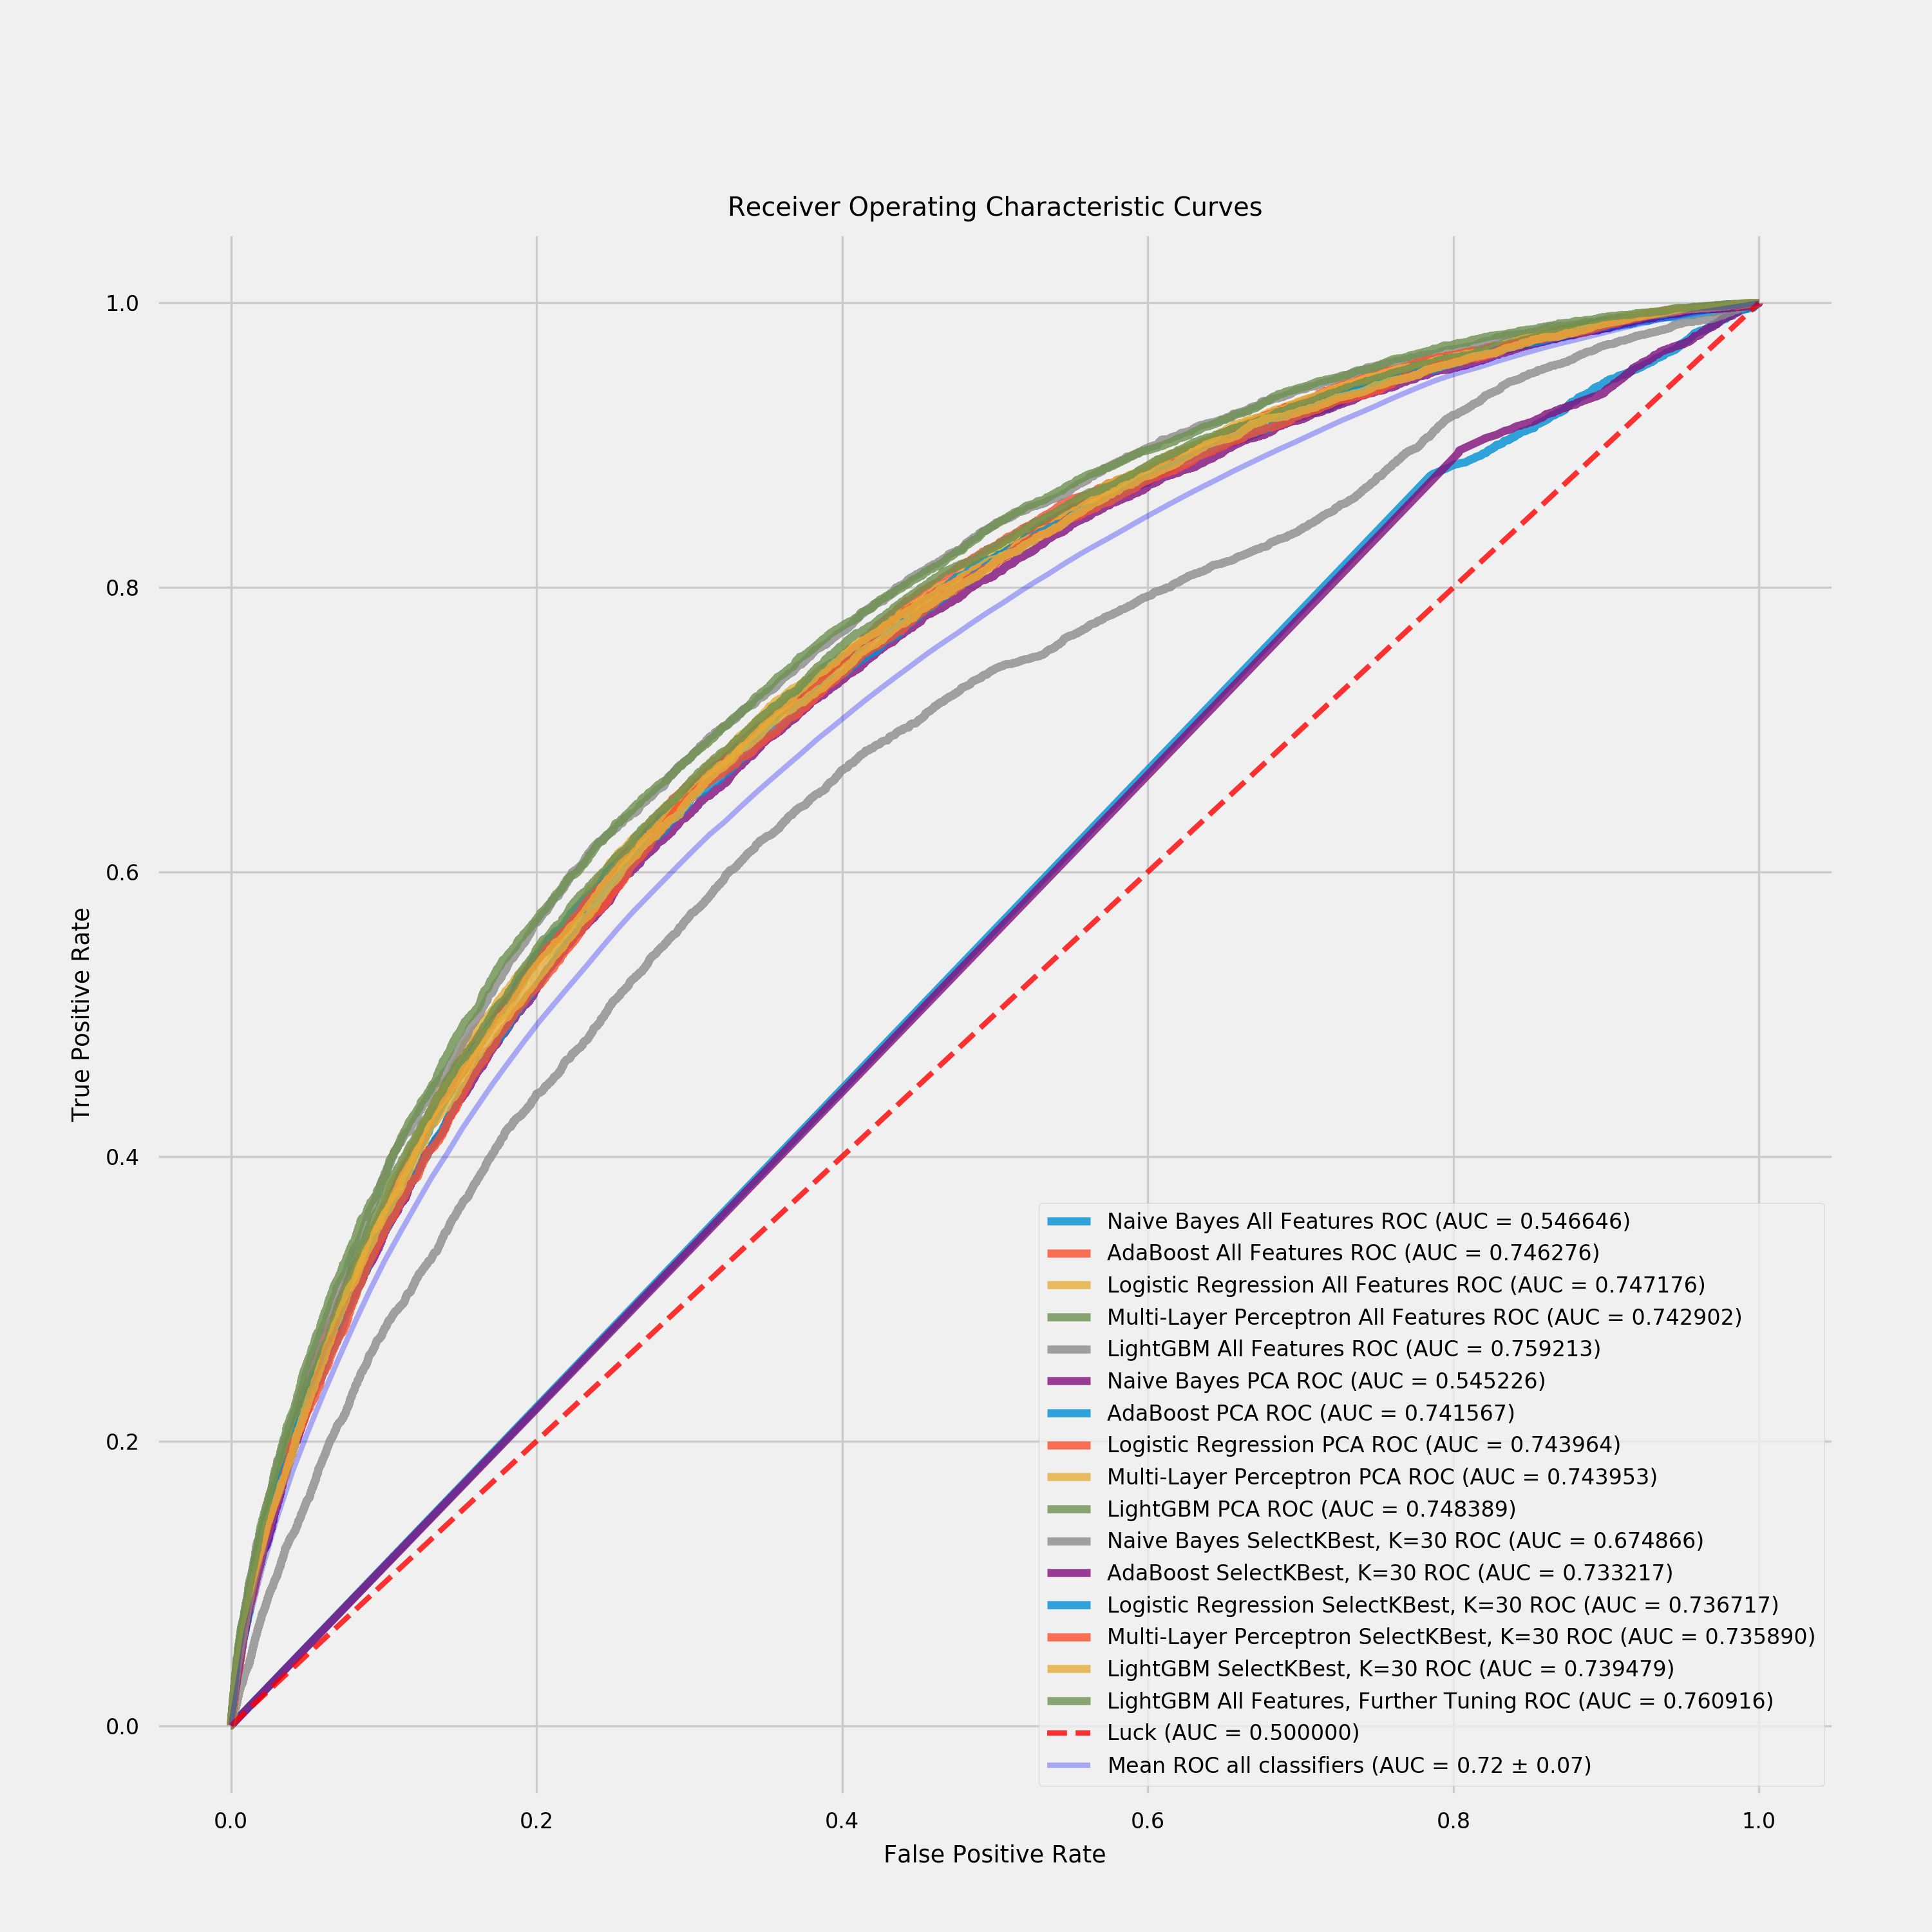
\includegraphics[width=\textwidth]{ReceiverOperatingCharacteristicCurves}
\centering
\caption{ROC Curves of each classifier and featureset}
\end{figure}

The next plot displays the top 50 feature importances of the best performing LightGBM algorithm after it had been trained on the full featureset.

\pagebreak

\begin{figure}[h!]
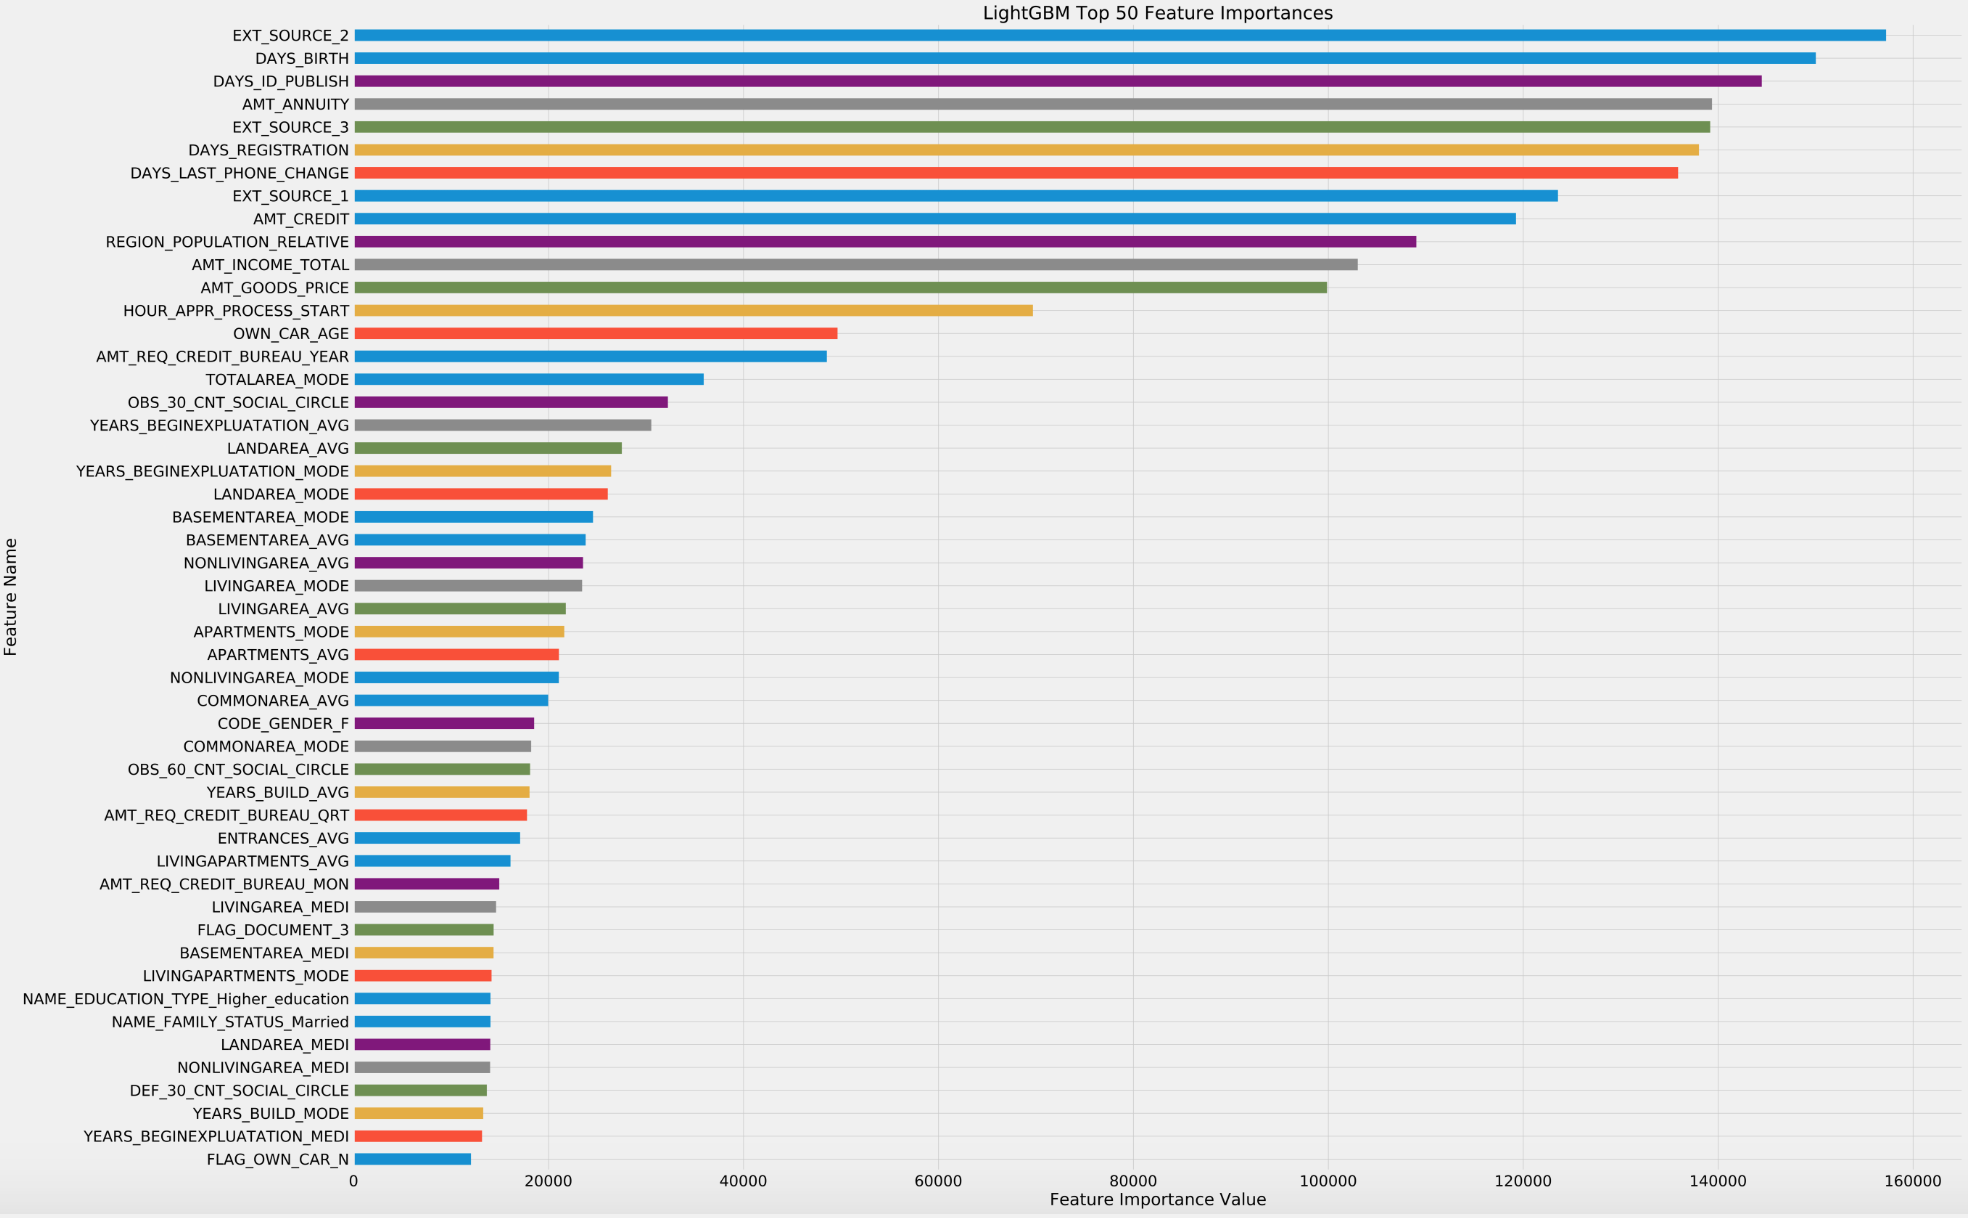
\includegraphics[width=\textwidth]{lightGBMFeatureImportances}
\centering
\caption{Top 50 feature importances of the best LightGBM model}
\end{figure}

The 15 most useful features for my LightGBM model are all numerical. Indeed, none of the three categorical features that I had engineered earlier made it into the top 50 features depicted above. If I had it to do all over again, I would have kept \colorbox{backcolor}{\textcolor{black}{\texttt{DAYS_EMPLOYED}}} as a numerical feature instead of re-engineering it into the binary \colorbox{backcolor}{\textcolor{black}{\texttt{HAS_JOB}}} feature.

\subsection{Reflection}
By far and away, the most challenging part of this project was understanding the dataset and all the quirks of its various features. I budgeted the majority of my time toward understanding what information each feature contained, how this information was distributed, and what sort of preprocessing techniques would need to be applied.

Dealing with the dataset's overabundance of missing values, or `NaN' entries, proved to be trickiest part of the data preprocessing phase. Most machine learning algorithms aren't designed to overlook missing entries, and so I had no choice but to come up with a strategy to work around this. I ultimately decided it was wisest to make a first attempt that used all the dataset's features, imputing any missing `NaN' values in numerical and categorical features according to the conventions and processes that seemed most reasonable to me. If I had more time, I would have liked to experiment with omitting some of the features with the most `Nan' values, or perhaps experimenting with different approaches to imputing missing values.

The most straightforward part of my process was chooising which learning algorithm to use. LightGBM was head and shoulders above every other algorithm I tried, both in terms of speed of training and in terms of its final ROC AUC score. If I had access to more compute power, I might have tried out the XGBOOST algorithm as well, but facing the limitation of training my learning algorithm locally on my laptop, I felt that attempting LightGBM alone was more than adequate for my solution.

Finally, thanks to LightGBM's training speed, the process of tuning its hyperparameters wasn't terribly painful. I am confident that I was able to thoroughly explore the ranges most of the hyperparameters one-by-one. However, I did unfortunately have to leave one stone mostly un-turned: I wasn't able to fully explore the interrelationships between \textit{all} of LightGBM's hyperparameters. Although I did make some headway using GridSearchCV, I had to accept that given the compute limitations of my laptop, there was only so much investigation that could be accomplished.

\subsection{Improvement}
Absent any large-scale comprehensive exploration of LightGBM's hyperparameters using GridSearchCV, I don't believe that there is much more to be gained from continuing to tweak my model's hyperparameters.

Instead, I believe that the lowest hanging fruit would be for me to bring into my dataset all the features from the six other data tables provided by Home Credit. After noticing how my model's ROC AUC score increased as I broadened the scope of features on which it was trained, I couldn't help but wonder if adding features from the data tables I had originally declined to include in this project might help my model's performance get that much closer to the current highest submissions on Kaggle.

Additionally, while researching various techniques that I might apply to this project, I came across a type of ensemble generation called stacking. In a nutshell, stacking is a method for building a learning ensemble that combines the predictive powers of several machine learning algorithms. The individual base level learning algorithms are each first trained on the training dataset. And the reason this technique is called stacking is because once this first round of training is complete, a higher level algorithm, or meta-model, is trained that uses the outputs of the base level models as input features.\cite{statsandbots}

I am hopeful that ensemble learning methods, such as stacking, will help close the gap between my model's current performance and the higher scores on the competition's leaderboard.

\begin{appendices}
\section{Data Table Descriptions}
\label{appendix:datatabledescriptions}
From the \href{https://www.kaggle.com/c/home-credit-default-risk/data}{data description page} on the Home Credit Kaggle competition's website\cite{kagglehomecreditcompetitiondata}.
\begin{enumerate}
  \item \textbf{application_\{train \textbar~test\}.csv}
    \begin{itemize}
      \item This is the main table, broken into two files for Train (with TARGET) and Test (without TARGET).
      \item Static data for all applications. One row represents one loan in our data sample.
    \end{itemize}
  \item \textbf{bureau.csv}
    \begin{itemize}
      \item All client's previous credits provided by other financial institutions that were reported to Credit Bureau (for clients who have a loan in our sample).
      \item For every loan in our sample, there are as many rows as number of credits the client had in Credit Bureau before the application date.
    \end{itemize}
  \item \textbf{bureau_balance.csv}
    \begin{itemize}
      \item Monthly balances of previous credits in Credit Bureau.
      \item This table has one row for each month of history of every previous credit reported to Credit Bureau – i.e the table has (\#loans in sample \# of relative previous credits \# of months where we have some history observable for the previous credits) rows.
    \end{itemize}
  \item \textbf{previous_application.csv}
    \begin{itemize}
      \item All previous applications for Home Credit loans of clients who have loans in our sample.
      \item There is one row for each previous application related to loans in our data sample.
    \end{itemize}
  \item \textbf{POS_CASH_balance.csv}
    \begin{itemize}
      \item Monthly balance snapshots of previous POS (point of sales) and cash loans that the applicant had with Home Credit.
      \item This table has one row for each month of history of every previous credit in Home Credit (consumer credit and cash loans) related to loans in our sample – i.e. the table has (\#loans in sample \# of relative previous credits \# of months in which we have some history observable for the previous credits) rows.
    \end{itemize}
  \item \textbf{installments_payments.csv}
    \begin{itemize}
      \item Repayment history for the previously disbursed credits in Home Credit related to the loans in our sample.
      \item There is a) one row for every payment that was made plus b) one row each for missed payment.
      \item One row is equivalent to one payment of one installment OR one installment corresponding to one payment of one previous Home Credit credit related to loans in our sample.
    \end{itemize}
  \item \textbf{credit_card_balance.csv}
    \begin{itemize}
      \item Monthly balance snapshots of previous credit cards that the applicant has with Home Credit.
      \item This table has one row for each month of history of every previous credit in Home Credit (consumer credit and cash loans) related to loans in our sample – i.e. the table has (\#loans in sample \# of relative previous credit cards \# of months where we have some history observable for the previous credit card) rows.
    \end{itemize}
\end{enumerate}

\section{Data Table Features}
\label{appendix:datatablefeatures}
From the HomeCredit_columns_description.csv file on the \href{https://www.kaggle.com/c/home-credit-default-risk/data}{data description page} on the Home Credit Kaggle competition's website\cite{kagglehomecreditcompetitiondata}.
\subsection{Main Data Table Features (application_\{train \textbar~test\}.csv)}
\begin{enumerate}
  \item \textbf{SK_ID_CURR}: ID of loan in our sample
  \item \textbf{TARGET}: Target variable (1 - client with payment difficulties: he/she had late payment more than X days on at least one of the first Y installments of the loan in our sample, 0 - all other cases)
  \item \textbf{NAME_CONTRACT_TYPE}: Identification if loan is cash or revolving
  \item \textbf{CODE_GENDER}: Gender of the client
  \item \textbf{FLAG_OWN_CAR}: Flag if the client owns a car
  \item \textbf{FLAG_OWN_REALTY}: Flag if client owns a house or flat
  \item \textbf{CNT_CHILDREN}: Number of children the client has
  \item \textbf{AMT_INCOME_TOTAL}: Income of the client
  \item \textbf{AMT_CREDIT}: Credit amount of the loan
  \item \textbf{AMT_ANNUITY}: Loan annuity
  \item \textbf{AMT_GOODS_PRICE}: For consumer loans it is the price of the goods for which the loan is given
  \item \textbf{NAME_TYPE_SUITE}: Who was accompanying client when he was applying for the loan
  \item \textbf{NAME_INCOME_TYPE}: Clients income type (businessman, working, maternity leave,Ö)
  \item \textbf{NAME_EDUCATION_TYPE}: Level of highest education the client achieved
  \item \textbf{NAME_FAMILY_STATUS}: Family status of the client
  \item \textbf{NAME_HOUSING_TYPE}: What is the housing situation of the client (renting, living with parents, ...)
  \item \textbf{REGION_POPULATION_RELATIVE}: Normalized population of region where client lives (higher number means the client lives in more populated region) -- normalized (although distribution is normal with minimal skewness, values are in approximate range [0.00,0.07] -- this is the only normalized feature in the main data table not distributed over the range [0,1])
  \item \textbf{DAYS_BIRTH}: Client's age in days at the time of application -- time only relative to the application
  \item \textbf{DAYS_EMPLOYED}: How many days before the application the person started current employment -- time only relative to the application
  \item \textbf{DAYS_REGISTRATION}: How many days before the application did client change his registration -- time only relative to the application
  \item \textbf{DAYS_ID_PUBLISH}: How many days before the application did client change the identity document with which he applied for the loan -- time only relative to the application
  \item \textbf{OWN_CAR_AGE}: Age of client's car
  \item \textbf{FLAG_MOBIL}: Did client provide mobile phone (1=YES, 0=NO)
  \item \textbf{FLAG_EMP_PHONE}: Did client provide work phone (1=YES, 0=NO)
  \item \textbf{FLAG_WORK_PHONE}: Did client provide home phone (1=YES, 0=NO)
  \item \textbf{FLAG_CONT_MOBILE}: Was mobile phone reachable (1=YES, 0=NO)
  \item \textbf{FLAG_PHONE}: Did client provide home phone (1=YES, 0=NO)
  \item \textbf{FLAG_EMAIL}: Did client provide email (1=YES, 0=NO)
  \item \textbf{OCCUPATION_TYPE}: What kind of occupation does the client have
  \item \textbf{CNT_FAM_MEMBERS}: How many family members does client have
  \item \textbf{REGION_RATING_CLIENT}: Our rating of the region where client lives (1,2,3)
  \item \textbf{REGION_RATING_CLIENT_W_CITY}: Our rating of the region where client lives with taking city into account (1,2,3)
  \item \textbf{WEEKDAY_APPR_PROCESS_START}: On which day of the week did the client apply for the loan
  \item \textbf{HOUR_APPR_PROCESS_START}: Approximately at what hour did the client apply for the loan	rounded
  \item \textbf{REG_REGION_NOT_LIVE_REGION}: Flag if client's permanent address does not match contact address (1=different, 0=same, at region level)
  \item \textbf{REG_REGION_NOT_WORK_REGION}: Flag if client's permanent address does not match work address (1=different, 0=same, at region level)
  \item \textbf{LIVE_REGION_NOT_WORK_REGION}: Flag if client's contact address does not match work address (1=different, 0=same, at region level)
  \item \textbf{REG_CITY_NOT_LIVE_CITY}: Flag if client's permanent address does not match contact address (1=different, 0=same, at city level)
  \item \textbf{REG_CITY_NOT_WORK_CITY}: Flag if client's permanent address does not match work address (1=different, 0=same, at city level)
  \item \textbf{LIVE_CITY_NOT_WORK_CITY}: Flag if client's contact address does not match work address (1=different, 0=same, at city level)
  \item \textbf{ORGANIZATION_TYPE}: Type of organization where client works
  \item \textbf{EXT_SOURCE_1}: Normalized score from external data source -- normalized, scaled to range [0,1]
  \item \textbf{EXT_SOURCE_2}: Normalized score from external data source -- normalized, scaled to range [0,1]
  \item \textbf{EXT_SOURCE_3}: Normalized score from external data source -- normalized, scaled to range [0,1]
  \item \textbf{APARTMENTS_AVG}: Normalized information about building where the client lives, What is average (_AVG suffix), modus (_MODE suffix), median (_MEDI suffix) apartment size, common area, living area, age of building, number of elevators, number of entrances, state of the building, number of floor -- normalized, scaled to range [0,1]
  \item \textbf{BASEMENTAREA_AVG}: Normalized information about building where the client lives, What is average (_AVG suffix), modus (_MODE suffix), median (_MEDI suffix) apartment size, common area, living area, age of building, number of elevators, number of entrances, state of the building, number of floor -- normalized, scaled to range [0,1]
  \item \textbf{YEARS_BEGINEXPLUATATION_AVG}: Normalized information about building where the client lives, What is average (_AVG suffix), modus (_MODE suffix), median (_MEDI suffix) apartment size, common area, living area, age of building, number of elevators, number of entrances, state of the building, number of floor -- normalized, scaled to range [0,1]
  \item \textbf{YEARS_BUILD_AVG}: Normalized information about building where the client lives, What is average (_AVG suffix), modus (_MODE suffix), median (_MEDI suffix) apartment size, common area, living area, age of building, number of elevators, number of entrances, state of the building, number of floor -- normalized, scaled to range [0,1]
  \item \textbf{COMMONAREA_AVG}: Normalized information about building where the client lives, What is average (_AVG suffix), modus (_MODE suffix), median (_MEDI suffix) apartment size, common area, living area, age of building, number of elevators, number of entrances, state of the building, number of floor -- normalized, scaled to range [0,1]
  \item \textbf{ELEVATORS_AVG}: Normalized information about building where the client lives, What is average (_AVG suffix), modus (_MODE suffix), median (_MEDI suffix) apartment size, common area, living area, age of building, number of elevators, number of entrances, state of the building, number of floor -- normalized, scaled to range [0,1]
  \item \textbf{ENTRANCES_AVG}: Normalized information about building where the client lives, What is average (_AVG suffix), modus (_MODE suffix), median (_MEDI suffix) apartment size, common area, living area, age of building, number of elevators, number of entrances, state of the building, number of floor -- normalized, scaled to range [0,1]
  \item \textbf{FLOORSMAX_AVG}: Normalized information about building where the client lives, What is average (_AVG suffix), modus (_MODE suffix), median (_MEDI suffix) apartment size, common area, living area, age of building, number of elevators, number of entrances, state of the building, number of floor -- normalized, scaled to range [0,1]
  \item \textbf{FLOORSMIN_AVG}: Normalized information about building where the client lives, What is average (_AVG suffix), modus (_MODE suffix), median (_MEDI suffix) apartment size, common area, living area, age of building, number of elevators, number of entrances, state of the building, number of floor -- normalized, scaled to range [0,1]
  \item \textbf{LANDAREA_AVG}: Normalized information about building where the client lives, What is average (_AVG suffix), modus (_MODE suffix), median (_MEDI suffix) apartment size, common area, living area, age of building, number of elevators, number of entrances, state of the building, number of floor -- normalized, scaled to range [0,1]
  \item \textbf{LIVINGAPARTMENTS_AVG}: Normalized information about building where the client lives, What is average (_AVG suffix), modus (_MODE suffix), median (_MEDI suffix) apartment size, common area, living area, age of building, number of elevators, number of entrances, state of the building, number of floor -- normalized, scaled to range [0,1]
  \item \textbf{LIVINGAREA_AVG}: Normalized information about building where the client lives, What is average (_AVG suffix), modus (_MODE suffix), median (_MEDI suffix) apartment size, common area, living area, age of building, number of elevators, number of entrances, state of the building, number of floor -- normalized, scaled to range [0,1]
  \item \textbf{NONLIVINGAPARTMENTS_AVG}: Normalized information about building where the client lives, What is average (_AVG suffix), modus (_MODE suffix), median (_MEDI suffix) apartment size, common area, living area, age of building, number of elevators, number of entrances, state of the building, number of floor -- normalized, scaled to range [0,1]
  \item \textbf{NONLIVINGAREA_AVG}: Normalized information about building where the client lives, What is average (_AVG suffix), modus (_MODE suffix), median (_MEDI suffix) apartment size, common area, living area, age of building, number of elevators, number of entrances, state of the building, number of floor -- normalized, scaled to range [0,1]
  \item \textbf{APARTMENTS_MODE}: Normalized information about building where the client lives, What is average (_AVG suffix), modus (_MODE suffix), median (_MEDI suffix) apartment size, common area, living area, age of building, number of elevators, number of entrances, state of the building, number of floor -- normalized, scaled to range [0,1]
  \item \textbf{BASEMENTAREA_MODE}: Normalized information about building where the client lives, What is average (_AVG suffix), modus (_MODE suffix), median (_MEDI suffix) apartment size, common area, living area, age of building, number of elevators, number of entrances, state of the building, number of floor -- normalized, scaled to range [0,1]
  \item \textbf{YEARS_BEGINEXPLUATATION_MODE}: Normalized information about building where the client lives, What is average (_AVG suffix), modus (_MODE suffix), median (_MEDI suffix) apartment size, common area, living area, age of building, number of elevators, number of entrances, state of the building, number of floor -- normalized, scaled to range [0,1]
  \item \textbf{YEARS_BUILD_MODE}: Normalized information about building where the client lives, What is average (_AVG suffix), modus (_MODE suffix), median (_MEDI suffix) apartment size, common area, living area, age of building, number of elevators, number of entrances, state of the building, number of floor -- normalized, scaled to range [0,1]
  \item \textbf{COMMONAREA_MODE}: Normalized information about building where the client lives, What is average (_AVG suffix), modus (_MODE suffix), median (_MEDI suffix) apartment size, common area, living area, age of building, number of elevators, number of entrances, state of the building, number of floor -- normalized, scaled to range [0,1]
  \item \textbf{ELEVATORS_MODE}: Normalized information about building where the client lives, What is average (_AVG suffix), modus (_MODE suffix), median (_MEDI suffix) apartment size, common area, living area, age of building, number of elevators, number of entrances, state of the building, number of floor -- normalized, scaled to range [0,1]
  \item \textbf{ENTRANCES_MODE}: Normalized information about building where the client lives, What is average (_AVG suffix), modus (_MODE suffix), median (_MEDI suffix) apartment size, common area, living area, age of building, number of elevators, number of entrances, state of the building, number of floor -- normalized, scaled to range [0,1]
  \item \textbf{FLOORSMAX_MODE}: Normalized information about building where the client lives, What is average (_AVG suffix), modus (_MODE suffix), median (_MEDI suffix) apartment size, common area, living area, age of building, number of elevators, number of entrances, state of the building, number of floor -- normalized, scaled to range [0,1]
  \item \textbf{FLOORSMIN_MODE}: Normalized information about building where the client lives, What is average (_AVG suffix), modus (_MODE suffix), median (_MEDI suffix) apartment size, common area, living area, age of building, number of elevators, number of entrances, state of the building, number of floor -- normalized, scaled to range [0,1]
  \item \textbf{LANDAREA_MODE}: Normalized information about building where the client lives, What is average (_AVG suffix), modus (_MODE suffix), median (_MEDI suffix) apartment size, common area, living area, age of building, number of elevators, number of entrances, state of the building, number of floor -- normalized, scaled to range [0,1]
  \item \textbf{LIVINGAPARTMENTS_MODE}: Normalized information about building where the client lives, What is average (_AVG suffix), modus (_MODE suffix), median (_MEDI suffix) apartment size, common area, living area, age of building, number of elevators, number of entrances, state of the building, number of floor -- normalized, scaled to range [0,1]
  \item \textbf{LIVINGAREA_MODE}: Normalized information about building where the client lives, What is average (_AVG suffix), modus (_MODE suffix), median (_MEDI suffix) apartment size, common area, living area, age of building, number of elevators, number of entrances, state of the building, number of floor -- normalized, scaled to range [0,1]
  \item \textbf{NONLIVINGAPARTMENTS_MODE}: Normalized information about building where the client lives, What is average (_AVG suffix), modus (_MODE suffix), median (_MEDI suffix) apartment size, common area, living area, age of building, number of elevators, number of entrances, state of the building, number of floor -- normalized, scaled to range [0,1]
  \item \textbf{NONLIVINGAREA_MODE}: Normalized information about building where the client lives, What is average (_AVG suffix), modus (_MODE suffix), median (_MEDI suffix) apartment size, common area, living area, age of building, number of elevators, number of entrances, state of the building, number of floor -- normalized, scaled to range [0,1]
  \item \textbf{APARTMENTS_MEDI}: Normalized information about building where the client lives, What is average (_AVG suffix), modus (_MODE suffix), median (_MEDI suffix) apartment size, common area, living area, age of building, number of elevators, number of entrances, state of the building, number of floor -- normalized, scaled to range [0,1]
  \item \textbf{BASEMENTAREA_MEDI}: Normalized information about building where the client lives, What is average (_AVG suffix), modus (_MODE suffix), median (_MEDI suffix) apartment size, common area, living area, age of building, number of elevators, number of entrances, state of the building, number of floor -- normalized, scaled to range [0,1]
  \item \textbf{YEARS_BEGINEXPLUATATION_MEDI}: Normalized information about building where the client lives, What is average (_AVG suffix), modus (_MODE suffix), median (_MEDI suffix) apartment size, common area, living area, age of building, number of elevators, number of entrances, state of the building, number of floor -- normalized, scaled to range [0,1]
  \item \textbf{YEARS_BUILD_MEDI}: Normalized information about building where the client lives, What is average (_AVG suffix), modus (_MODE suffix), median (_MEDI suffix) apartment size, common area, living area, age of building, number of elevators, number of entrances, state of the building, number of floor -- normalized, scaled to range [0,1]
  \item \textbf{COMMONAREA_MEDI}: Normalized information about building where the client lives, What is average (_AVG suffix), modus (_MODE suffix), median (_MEDI suffix) apartment size, common area, living area, age of building, number of elevators, number of entrances, state of the building, number of floor -- normalized, scaled to range [0,1]
  \item \textbf{ELEVATORS_MEDI}: Normalized information about building where the client lives, What is average (_AVG suffix), modus (_MODE suffix), median (_MEDI suffix) apartment size, common area, living area, age of building, number of elevators, number of entrances, state of the building, number of floor -- normalized, scaled to range [0,1]
  \item \textbf{ENTRANCES_MEDI}: Normalized information about building where the client lives, What is average (_AVG suffix), modus (_MODE suffix), median (_MEDI suffix) apartment size, common area, living area, age of building, number of elevators, number of entrances, state of the building, number of floor -- normalized, scaled to range [0,1]
  \item \textbf{FLOORSMAX_MEDI}: Normalized information about building where the client lives, What is average (_AVG suffix), modus (_MODE suffix), median (_MEDI suffix) apartment size, common area, living area, age of building, number of elevators, number of entrances, state of the building, number of floor -- normalized, scaled to range [0,1]
  \item \textbf{FLOORSMIN_MEDI}: Normalized information about building where the client lives, What is average (_AVG suffix), modus (_MODE suffix), median (_MEDI suffix) apartment size, common area, living area, age of building, number of elevators, number of entrances, state of the building, number of floor -- normalized, scaled to range [0,1]
  \item \textbf{LANDAREA_MEDI}: Normalized information about building where the client lives, What is average (_AVG suffix), modus (_MODE suffix), median (_MEDI suffix) apartment size, common area, living area, age of building, number of elevators, number of entrances, state of the building, number of floor -- normalized, scaled to range [0,1]
  \item \textbf{LIVINGAPARTMENTS_MEDI}: Normalized information about building where the client lives, What is average (_AVG suffix), modus (_MODE suffix), median (_MEDI suffix) apartment size, common area, living area, age of building, number of elevators, number of entrances, state of the building, number of floor -- normalized, scaled to range [0,1]
  \item \textbf{LIVINGAREA_MEDI}: Normalized information about building where the client lives, What is average (_AVG suffix), modus (_MODE suffix), median (_MEDI suffix) apartment size, common area, living area, age of building, number of elevators, number of entrances, state of the building, number of floor -- normalized, scaled to range [0,1]
  \item \textbf{NONLIVINGAPARTMENTS_MEDI}: Normalized information about building where the client lives, What is average (_AVG suffix), modus (_MODE suffix), median (_MEDI suffix) apartment size, common area, living area, age of building, number of elevators, number of entrances, state of the building, number of floor -- normalized, scaled to range [0,1]
  \item \textbf{NONLIVINGAREA_MEDI}: Normalized information about building where the client lives, What is average (_AVG suffix), modus (_MODE suffix), median (_MEDI suffix) apartment size, common area, living area, age of building, number of elevators, number of entrances, state of the building, number of floor -- normalized, scaled to range [0,1]
  \item \textbf{FONDKAPREMONT_MODE}: Categorical -- unclear exactly what this feature indicates. Examples of entries include ``reg oper account," ``reg oper spec account," ``org spec account." (Originally mislabeled by Home Credit as ``Normalized information about building where the client lives.")
  \item \textbf{HOUSETYPE_MODE}: Categorical -- type of residence applicant lives in. (Originally mislabeled by Home Credit as ``Normalized information about building where the client lives.")
  \item \textbf{TOTALAREA_MODE}: Normalized information about building where the client lives, What is average (_AVG suffix), modus (_MODE suffix), median (_MEDI suffix) apartment size, common area, living area, age of building, number of elevators, number of entrances, state of the building, number of floor -- normalized, scaled to range [0,1]
  \item \textbf{WALLSMATERIAL_MODE}: Categorical -- type of material that the walls in applicant's residence are made of. (Originally mislabeled by Home Credit as ``Normalized information about building where the client lives.")
  \item \textbf{EMERGENCYSTATE_MODE}: Categorical -- unclear exactly what this feature indicates. Examples of entries include ``Yes" and ``No." (Originally mislabeled by Home Credit as ``Normalized information about building where the client lives.")
  \item \textbf{OBS_30_CNT_SOCIAL_CIRCLE}: How many observation of client's social surroundings with observable 30 DPD (days past due) default
  \item \textbf{DEF_30_CNT_SOCIAL_CIRCLE}: How many observation of client's social surroundings defaulted on 30 DPD (days past due)
  \item \textbf{OBS_60_CNT_SOCIAL_CIRCLE}: How many observation of client's social surroundings with observable 60 DPD (days past due) default
  \item \textbf{DEF_60_CNT_SOCIAL_CIRCLE}: How many observation of client's social surroundings defaulted on 60 (days past due) DPD
  \item \textbf{DAYS_LAST_PHONE_CHANGE}: How many days before application did client change phone
  \item \textbf{FLAG_DOCUMENT_2}: Did client provide document 2
  \item \textbf{FLAG_DOCUMENT_3}: Did client provide document 3
  \item \textbf{FLAG_DOCUMENT_4}: Did client provide document 4
  \item \textbf{FLAG_DOCUMENT_5}: Did client provide document 5
  \item \textbf{FLAG_DOCUMENT_6}: Did client provide document 6
  \item \textbf{FLAG_DOCUMENT_7}: Did client provide document 7
  \item \textbf{FLAG_DOCUMENT_8}: Did client provide document 8
  \item \textbf{FLAG_DOCUMENT_9}: Did client provide document 9
  \item \textbf{FLAG_DOCUMENT_10}: Did client provide document 10
  \item \textbf{FLAG_DOCUMENT_11}: Did client provide document 11
  \item \textbf{FLAG_DOCUMENT_12}: Did client provide document 12
  \item \textbf{FLAG_DOCUMENT_13}: Did client provide document 13
  \item \textbf{FLAG_DOCUMENT_14}: Did client provide document 14
  \item \textbf{FLAG_DOCUMENT_15}: Did client provide document 15
  \item \textbf{FLAG_DOCUMENT_16}: Did client provide document 16
  \item \textbf{FLAG_DOCUMENT_17}: Did client provide document 17
  \item \textbf{FLAG_DOCUMENT_18}: Did client provide document 18
  \item \textbf{FLAG_DOCUMENT_19}: Did client provide document 19
  \item \textbf{FLAG_DOCUMENT_20}: Did client provide document 20
  \item \textbf{FLAG_DOCUMENT_21}: Did client provide document 21
  \item \textbf{AMT_REQ_CREDIT_BUREAU_HOUR}: Number of enquiries to Credit Bureau about the client one hour before application
  \item \textbf{AMT_REQ_CREDIT_BUREAU_DAY}: Number of enquiries to Credit Bureau about the client one day before application (excluding one hour before application)
  \item \textbf{AMT_REQ_CREDIT_BUREAU_WEEK}: Number of enquiries to Credit Bureau about the client one week before application (excluding one day before application)
  \item \textbf{AMT_REQ_CREDIT_BUREAU_MON}: Number of enquiries to Credit Bureau about the client one month before application (excluding one week before application)
  \item \textbf{AMT_REQ_CREDIT_BUREAU_QRT}: Number of enquiries to Credit Bureau about the client 3 month before application (excluding one month before application)
  \item \textbf{AMT_REQ_CREDIT_BUREAU_YEAR}: Number of enquiries to Credit Bureau about the client one day year (excluding last 3 months before application)
\end{enumerate}

\subsection{Bureau Data Table Features (bureau.csv)}
\label{bureaudatatablefeatures}
\begin{enumerate}
  \item \textbf{SK_ID_CURR}: ID of loan in our sample - one loan in our sample can have 0,1,2 or more related previous credits in credit bureau -- hashed
  \item \textbf{SK_ID_BUREAU}: Recoded ID of previous Credit Bureau credit related to our loan (unique coding for each loan application) -- hashed
  \item \textbf{CREDIT_ACTIVE}: Status of the Credit Bureau (CB) reported credits
  \item \textbf{CREDIT_CURRENCY}: Recoded currency of the Credit Bureau credit -- recoded
  \item \textbf{DAYS_CREDIT}: How many days before current application did client apply for Credit Bureau credit -- time only relative to the application
  \item \textbf{CREDIT_DAY_OVERDUE}: Number of days past due on CB credit at the time of application for related loan in our sample
  \item \textbf{DAYS_CREDIT_ENDDATE}: Remaining duration of CB credit (in days) at the time of application in Home Credit -- time only relative to the application
  \item \textbf{DAYS_ENDDATE_FACT}: Days since CB credit ended at the time of application in Home Credit (only for closed credit) -- time only relative to the application
  \item \textbf{AMT_CREDIT_MAX_OVERDUE}: Maximal amount overdue on the Credit Bureau credit so far (at application date of loan in our sample)
  \item \textbf{CNT_CREDIT_PROLONG}: How many times was the Credit Bureau credit prolonged
  \item \textbf{AMT_CREDIT_SUM}: Current credit amount for the Credit Bureau credit
  \item \textbf{AMT_CREDIT_SUM_DEBT}: Current debt on Credit Bureau credit
  \item \textbf{AMT_CREDIT_SUM_LIMIT}: Current credit limit of credit card reported in Credit Bureau
  \item \textbf{AMT_CREDIT_SUM_OVERDUE}: Current amount overdue on Credit Bureau credit
  \item \textbf{CREDIT_TYPE}: Type of Credit Bureau credit (Car, cash,...)
  \item \textbf{DAYS_CREDIT_UPDATE}: How many days before loan application did last information about the Credit Bureau credit come -- time only relative to the application
  \item \textbf{AMT_ANNUITY}: Annuity of the Credit Bureau credit
\end{enumerate}

\subsection{Bureau Balance Data Table Features (bureau_balance.csv)}
\label{bureaubalancedatatablefeatures}
\begin{enumerate}
  \item \textbf{SK_ID_BUREAU}: Recoded ID of Credit Bureau credit (unique coding for each application) - use this to join to CREDIT_BUREAU table -- hashed
  \item \textbf{MONTHS_BALANCE}: Month of balance relative to application date (-1 means the freshest balance date) -- time only relative to the application
  \item \textbf{STATUS}: Status of Credit Bureau loan during the month (active, closed, DPD0-30,Ö [C means closed, X means status unknown, 0 means no DPD, 1 means maximal did during month between 1-30, 2 means DPD 31-60,Ö 5 means DPD 120+ or sold or written off ])
\end{enumerate}

\subsection{Previous Application Data Table Features (previous_application.csv)}
\begin{enumerate}
  \item \textbf{SK_ID_PREV}: ID of previous credit in Home credit related to loan in our sample. (One loan in our sample can have 0,1,2 or more previous loan applications in Home Credit, previous application could, but not necessarily have to lead to credit) -- hashed
  \item \textbf{SK_ID_CURR}: ID of loan in our sample -- hashed
  \item \textbf{NAME_CONTRACT_TYPE}: Contract product type (Cash loan, consumer loan [POS] ,...) of the previous application
  \item \textbf{AMT_ANNUITY}: Annuity of previous application
  \item \textbf{AMT_APPLICATION}: For how much credit did client ask on the previous application
  \item \textbf{AMT_CREDIT}: Final credit amount on the previous application. This differs from AMT_APPLICATION in a way that the AMT_APPLICATION is the amount for which the client initially applied for, but during our approval process he could have received different amount - AMT_CREDIT
  \item \textbf{AMT_DOWN_PAYMENT}: Down payment on the previous application
  \item \textbf{AMT_GOODS_PRICE}: Goods price of good that client asked for (if applicable) on the previous application
  \item \textbf{WEEKDAY_APPR_PROCESS_START}: On which day of the week did the client apply for previous application
  \item \textbf{HOUR_APPR_PROCESS_START}: Approximately at what day hour did the client apply for the previous application -- rounded
  \item \textbf{FLAG_LAST_APPL_PER_CONTRACT}: Flag if it was last application for the previous contract. Sometimes by mistake of client or our clerk there could be more applications for one single contract
  \item \textbf{NFLAG_LAST_APPL_IN_DAY}: Flag if the application was the last application per day of the client. Sometimes clients apply for more applications a day. Rarely it could also be error in our system that one application is in the database twice
  \item \textbf{RATE_DOWN_PAYMENT}: Down payment rate normalized on previous credit -- normalized
  \item \textbf{RATE_INTEREST_PRIMARY}: Interest rate normalized on previous credit -- normalized
  \item \textbf{RATE_INTEREST_PRIVILEGED}: Interest rate normalized on previous credit -- normalized
  \item \textbf{NAME_CASH_LOAN_PURPOSE}: Purpose of the cash loan
  \item \textbf{NAME_CONTRACT_STATUS}: Contract status (approved, cancelled, ...) of previous application
  \item \textbf{DAYS_DECISION}: Relative to current application when was the decision about previous application made	time only relative to the application
  \item \textbf{NAME_PAYMENT_TYPE}: Payment method that client chose to pay for the previous application
  \item \textbf{CODE_REJECT_REASON}: Why was the previous application rejected
  \item \textbf{NAME_TYPE_SUITE}: Who accompanied client when applying for the previous application
  \item \textbf{NAME_CLIENT_TYPE}: Was the client old or new client when applying for the previous application
  \item \textbf{NAME_GOODS_CATEGORY}: What kind of goods did the client apply for in the previous application
  \item \textbf{NAME_PORTFOLIO}: Was the previous application for CASH, POS, CAR, Ö
  \item \textbf{NAME_PRODUCT_TYPE}: Was the previous application x-sell o walk-in
  \item \textbf{CHANNEL_TYPE}: Through which channel we acquired the client on the previous application
  \item \textbf{SELLERPLACE_AREA}: Selling area of seller place of the previous application
  \item \textbf{NAME_SELLER_INDUSTRY}: The industry of the seller
  \item \textbf{CNT_PAYMENT}: Term of previous credit at application of the previous application
  \item \textbf{NAME_YIELD_GROUP}: Grouped interest rate into small medium and high of the previous application -- grouped
  \item \textbf{PRODUCT_COMBINATION}: Detailed product combination of the previous application
  \item \textbf{DAYS_FIRST_DRAWING}: Relative to application date of current application when was the first disbursement of the previous application -- time only relative to the application
  \item \textbf{DAYS_FIRST_DUE}: Relative to application date of current application when was the first due supposed to be of the previous application -- time only relative to the application
  \item \textbf{DAYS_LAST_DUE_1ST_VERSION}: Relative to application date of current application when was the first due of the previous application -- time only relative to the application
  \item \textbf{DAYS_LAST_DUE}: Relative to application date of current application when was the last due date of the previous application -- time only relative to the application
  \item \textbf{DAYS_TERMINATION}: Relative to application date of current application when was the expected termination of the previous application -- time only relative to the application
  \item \textbf{NFLAG_INSURED_ON_APPROVAL}: Did the client requested insurance during the previous application
\end{enumerate}

\subsection{POS CASH Balance Data Table Features (POS_CASH_balance.csv)}
\begin{enumerate}
  \item \textbf{SK_ID_PREV}: ID of previous credit in Home Credit related to loan in our sample. (One loan in our sample can have 0,1,2 or more previous loans in Home Credit)
  \item \textbf{SK_ID_CURR}: ID of loan in our sample
  \item \textbf{MONTHS_BALANCE}: Month of balance relative to application date (-1 means the information to the freshest monthly snapshot, 0 means the information at application - often it will be the same as -1 as many banks are not updating the information to Credit Bureau regularly ) -- time only relative to the application
  \item \textbf{CNT_INSTALMENT}: Term of previous credit (can change over time)
  \item \textbf{CNT_INSTALMENT_FUTUR}: Installments left to pay on the previous credit
  \item \textbf{NAME_CONTRACT_STATUS}: Contract status during the month
  \item \textbf{SK_DPD}: DPD (days past due) during the month of previous credit
  \item \textbf{SK_DPD_DEF}: DPD during the month with tolerance (debts with low loan amounts are ignored) of the previous credit
\end{enumerate}

\subsection{Installments Payments Data Table Features (installments_payments.csv)}
\begin{enumerate}
  \item \textbf{SK_ID_PREV}: ID of previous credit in Home credit related to loan in our sample. (One loan in our sample can have 0,1,2 or more previous loans in Home Credit) -- hashed
  \item \textbf{SK_ID_CURR}: ID of loan in our sample -- hashed
  \item \textbf{NUM_INSTALMENT_VERSION}: Version of installment calendar (0 is for credit card) of previous credit. Change of installment version from month to month signifies that some parameter of payment calendar has changed
  \item \textbf{NUM_INSTALMENT_NUMBER}: On which installment we observe payment
  \item \textbf{DAYS_INSTALMENT}: When the installment of previous credit was supposed to be paid (relative to application date of current loan) -- time only relative to the application
  \item \textbf{DAYS_ENTRY_PAYMENT}: When was the installments of previous credit paid actually (relative to application date of current loan) -- time only relative to the application
  \item \textbf{AMT_INSTALMENT}: What was the prescribed installment amount of previous credit on this installment
  \item \textbf{AMT_PAYMENT}: What the client actually paid on previous credit on this installment
\end{enumerate}

\subsection{Credit Card Balance Data Table Features (credit_card_balance.csv)}
\begin{enumerate}
  \item \textbf{SK_ID_PREV}: ID of previous credit in Home credit related to loan in our sample. (One loan in our sample can have 0,1,2 or more previous loans in Home Credit) -- hashed
  \item \textbf{SK_ID_CURR}: ID of loan in our sample -- hashed
  \item \textbf{MONTHS_BALANCE}: Month of balance relative to application date (-1 means the freshest balance date) -- time only relative to the application
  \item \textbf{AMT_BALANCE}: Balance during the month of previous credit
  \item \textbf{AMT_CREDIT_LIMIT_ACTUAL}: Credit card limit during the month of the previous credit
  \item \textbf{AMT_DRAWINGS_ATM_CURRENT}: Amount drawing at ATM during the month of the previous credit
  \item \textbf{AMT_DRAWINGS_CURRENT}: Amount drawing during the month of the previous credit
  \item \textbf{AMT_DRAWINGS_OTHER_CURRENT}: Amount of other drawings during the month of the previous credit
  \item \textbf{AMT_DRAWINGS_POS_CURRENT}: Amount drawing or buying goods during the month of the previous credit
  \item \textbf{AMT_INST_MIN_REGULARITY}: Minimal installment for this month of the previous credit
  \item \textbf{AMT_PAYMENT_CURRENT}: How much did the client pay during the month on the previous credit
  \item \textbf{AMT_PAYMENT_TOTAL_CURRENT}: How much did the client pay during the month in total on the previous credit
  \item \textbf{AMT_RECEIVABLE_PRINCIPAL}: Amount receivable for principal on the previous credit
  \item \textbf{AMT_RECIVABLE}: Amount receivable on the previous credit
  \item \textbf{AMT_TOTAL_RECEIVABLE}: Total amount receivable on the previous credit
  \item \textbf{CNT_DRAWINGS_ATM_CURRENT}: Number of drawings at ATM during this month on the previous credit
  \item \textbf{CNT_DRAWINGS_CURRENT}: Number of drawings during this month on the previous credit
  \item \textbf{CNT_DRAWINGS_OTHER_CURRENT}: Number of other drawings during this month on the previous credit
  \item \textbf{CNT_DRAWINGS_POS_CURRENT}: Number of drawings for goods during this month on the previous credit
  \item \textbf{CNT_INSTALMENT_MATURE_CUM}: Number of paid installments on the previous credit
  \item \textbf{NAME_CONTRACT_STATUS}: Contract status (active signed,...) on the previous credit
  \item \textbf{SK_DPD}: DPD (Days past due) during the month on the previous credit
  \item \textbf{SK_DPD_DEF}: DPD (Days past due) during the month with tolerance (debts with low loan amounts are ignored) of the previous credit
\end{enumerate}

\section{Data Table Statistical Summaries}
\label{appendix:datatablestatsummaries}
\subsection{Main Data Table Statistical Summary (application_train.csv)}
\label{appendix:maindatatablestatsummary}

\tiny
\definecolor{lightgray}{gray}{0.92}
{\rowcolors{2}{white}{lightgray}
\begin{longtable}[c]{| l || r | r | r | r | r | r | r | r |}

 \caption{Main Data Table Statistical Summary\label{maindatatablestatsummary}}\\

 \hline
 \rowcolor{white} \multicolumn{9}{| c |}{\textbf{application_train.csv Feature Statistics}}\\
 \hline
 \rowcolor{white} \textbf{Feature} & \textbf{Count} & \textbf{Mean} & \textbf{Std} & \textbf{Min} & \textbf{25\%} & \textbf{50\%} & \textbf{75\%} & \textbf{Max}\\
 \hline
 \endfirsthead

 \rowcolor{white} \caption[]{Main Data Table Statistical Summary (continued)}\\
 \rowcolor{white} \hline
 \rowcolor{white} \multicolumn{9}{|c|}{\textbf{application_train.csv Feature Statistics}\ref{maindatatablestatsummary}}\\
 \hline
 \rowcolor{white} \textbf{Feature} & \textbf{Count} & \textbf{Mean} & \textbf{Std} & \textbf{Min} & \textbf{25\%} & \textbf{50\%} & \textbf{75\%} & \textbf{Max}\\
 \hline
 \endhead

 \hline
 \endfoot

 \hline
 \endlastfoot

 SK_ID_CURR	&	307511	&	278180.5186	&	102790.1753	&	1.00E+05	&	189145.5	&	278202	&	367142.5	&	4.56E+05	\\
 TARGET	&	307511	&	0.080729	&	0.272419	&	0.00E+00	&	0	&	0	&	0	&	1.00E+00	\\
 CNT_CHILDREN	&	307511	&	0.417052	&	0.722121	&	0.00E+00	&	0	&	0	&	1	&	1.90E+01	\\
 AMT_INCOME_TOTAL	&	307511	&	168797.9193	&	237123.1463	&	2.57E+04	&	112500	&	147150	&	202500	&	1.17E+08	\\
 AMT_CREDIT	&	307511	&	599025.9997	&	402490.777	&	4.50E+04	&	270000	&	513531	&	808650	&	4.05E+06	\\
 AMT_ANNUITY	&	307499	&	27108.57391	&	14493.73732	&	1.62E+03	&	16524	&	24903	&	34596	&	2.58E+05	\\
 AMT_GOODS_PRICE	&	307233	&	538396.2074	&	369446.4605	&	4.05E+04	&	238500	&	450000	&	679500	&	4.05E+06	\\
 REGION_POPULATION_RELATIVE	&	307511	&	0.020868	&	0.013831	&	2.90E-04	&	0.010006	&	0.01885	&	0.028663	&	7.25E-02	\\
 DAYS_BIRTH	&	307511	&	-16036.99507	&	4363.988632	&	-2.52E+04	&	-19682	&	-15750	&	-12413	&	-7.49E+03	\\
 DAYS_EMPLOYED	&	307511	&	63815.0459	&	141275.7665	&	-1.79E+04	&	-2760	&	-1213	&	-289	&	3.65E+05	\\
 DAYS_REGISTRATION	&	307511	&	-4986.120328	&	3522.886321	&	-2.47E+04	&	-7479.5	&	-4504	&	-2010	&	0.00E+00	\\
 DAYS_ID_PUBLISH	&	307511	&	-2994.202373	&	1509.450419	&	-7.20E+03	&	-4299	&	-3254	&	-1720	&	0.00E+00	\\
 OWN_CAR_AGE	&	104582	&	12.061091	&	11.944812	&	0.00E+00	&	5	&	9	&	15	&	9.10E+01	\\
 FLAG_MOBIL	&	307511	&	0.999997	&	0.001803	&	0.00E+00	&	1	&	1	&	1	&	1.00E+00	\\
 FLAG_EMP_PHONE	&	307511	&	0.819889	&	0.38428	&	0.00E+00	&	1	&	1	&	1	&	1.00E+00	\\
 FLAG_WORK_PHONE	&	307511	&	0.199368	&	0.399526	&	0.00E+00	&	0	&	0	&	0	&	1.00E+00	\\
 FLAG_CONT_MOBILE	&	307511	&	0.998133	&	0.043164	&	0.00E+00	&	1	&	1	&	1	&	1.00E+00	\\
 FLAG_PHONE	&	307511	&	0.281066	&	0.449521	&	0.00E+00	&	0	&	0	&	1	&	1.00E+00	\\
 FLAG_EMAIL	&	307511	&	0.05672	&	0.231307	&	0.00E+00	&	0	&	0	&	0	&	1.00E+00	\\
 CNT_FAM_MEMBERS	&	307509	&	2.152665	&	0.910682	&	1.00E+00	&	2	&	2	&	3	&	2.00E+01	\\
 REGION_RATING_CLIENT	&	307511	&	2.052463	&	0.509034	&	1.00E+00	&	2	&	2	&	2	&	3.00E+00	\\
 REGION_RATING_CLIENT_W_CITY	&	307511	&	2.031521	&	0.502737	&	1.00E+00	&	2	&	2	&	2	&	3.00E+00	\\
 HOUR_APPR_PROCESS_START	&	307511	&	12.063419	&	3.265832	&	0.00E+00	&	10	&	12	&	14	&	2.30E+01	\\
 REG_REGION_NOT_LIVE_REGION	&	307511	&	0.015144	&	0.122126	&	0.00E+00	&	0	&	0	&	0	&	1.00E+00	\\
 REG_REGION_NOT_WORK_REGION	&	307511	&	0.050769	&	0.219526	&	0.00E+00	&	0	&	0	&	0	&	1.00E+00	\\
 LIVE_REGION_NOT_WORK_REGION	&	307511	&	0.040659	&	0.197499	&	0.00E+00	&	0	&	0	&	0	&	1.00E+00	\\
 REG_CITY_NOT_LIVE_CITY	&	307511	&	0.078173	&	0.268444	&	0.00E+00	&	0	&	0	&	0	&	1.00E+00	\\
 REG_CITY_NOT_WORK_CITY	&	307511	&	0.230454	&	0.421124	&	0.00E+00	&	0	&	0	&	0	&	1.00E+00	\\
 LIVE_CITY_NOT_WORK_CITY	&	307511	&	0.179555	&	0.383817	&	0.00E+00	&	0	&	0	&	0	&	1.00E+00	\\
 EXT_SOURCE_1	&	134133	&	0.50213	&	0.211062	&	1.46E-02	&	0.334007	&	0.505998	&	0.675053	&	9.63E-01	\\
 EXT_SOURCE_2	&	306851	&	0.514393	&	0.19106	&	8.17E-08	&	0.392457	&	0.565961	&	0.663617	&	8.55E-01	\\
 EXT_SOURCE_3	&	246546	&	0.510853	&	0.194844	&	5.27E-04	&	0.37065	&	0.535276	&	0.669057	&	8.96E-01	\\
 APARTMENTS_AVG	&	151450	&	0.11744	&	0.10824	&	0.00E+00	&	0.0577	&	0.0876	&	0.1485	&	1.00E+00	\\
 BASEMENTAREA_AVG	&	127568	&	0.088442	&	0.082438	&	0.00E+00	&	0.0442	&	0.0763	&	0.1122	&	1.00E+00	\\
 YEARS_BEGINEXPLUATATION_AVG	&	157504	&	0.977735	&	0.059223	&	0.00E+00	&	0.9767	&	0.9816	&	0.9866	&	1.00E+00	\\
 YEARS_BUILD_AVG	&	103023	&	0.752471	&	0.11328	&	0.00E+00	&	0.6872	&	0.7552	&	0.8232	&	1.00E+00	\\
 COMMONAREA_AVG	&	92646	&	0.044621	&	0.076036	&	0.00E+00	&	0.0078	&	0.0211	&	0.0515	&	1.00E+00	\\
 ELEVATORS_AVG	&	143620	&	0.078942	&	0.134576	&	0.00E+00	&	0	&	0	&	0.12	&	1.00E+00	\\
 ENTRANCES_AVG	&	152683	&	0.149725	&	0.100049	&	0.00E+00	&	0.069	&	0.1379	&	0.2069	&	1.00E+00	\\
 FLOORSMAX_AVG	&	154491	&	0.226282	&	0.144641	&	0.00E+00	&	0.1667	&	0.1667	&	0.3333	&	1.00E+00	\\
 FLOORSMIN_AVG	&	98869	&	0.231894	&	0.16138	&	0.00E+00	&	0.0833	&	0.2083	&	0.375	&	1.00E+00	\\
 LANDAREA_AVG	&	124921	&	0.066333	&	0.081184	&	0.00E+00	&	0.0187	&	0.0481	&	0.0856	&	1.00E+00	\\
 LIVINGAPARTMENTS_AVG	&	97312	&	0.100775	&	0.092576	&	0.00E+00	&	0.0504	&	0.0756	&	0.121	&	1.00E+00	\\
 LIVINGAREA_AVG	&	153161	&	0.107399	&	0.110565	&	0.00E+00	&	0.0453	&	0.0745	&	0.1299	&	1.00E+00	\\
 NONLIVINGAPARTMENTS_AVG	&	93997	&	0.008809	&	0.047732	&	0.00E+00	&	0	&	0	&	0.0039	&	1.00E+00	\\
 NONLIVINGAREA_AVG	&	137829	&	0.028358	&	0.069523	&	0.00E+00	&	0	&	0.0036	&	0.0277	&	1.00E+00	\\
 APARTMENTS_MODE	&	151450	&	0.114231	&	0.107936	&	0.00E+00	&	0.0525	&	0.084	&	0.1439	&	1.00E+00	\\
 BASEMENTAREA_MODE	&	127568	&	0.087543	&	0.084307	&	0.00E+00	&	0.0407	&	0.0746	&	0.1124	&	1.00E+00	\\
 YEARS_BEGINEXPLUATATION_MODE	&	157504	&	0.977065	&	0.064575	&	0.00E+00	&	0.9767	&	0.9816	&	0.9866	&	1.00E+00	\\
 YEARS_BUILD_MODE	&	103023	&	0.759637	&	0.110111	&	0.00E+00	&	0.6994	&	0.7648	&	0.8236	&	1.00E+00	\\
 COMMONAREA_MODE	&	92646	&	0.042553	&	0.074445	&	0.00E+00	&	0.0072	&	0.019	&	0.049	&	1.00E+00	\\
 ELEVATORS_MODE	&	143620	&	0.07449	&	0.132256	&	0.00E+00	&	0	&	0	&	0.1208	&	1.00E+00	\\
 ENTRANCES_MODE	&	152683	&	0.145193	&	0.100977	&	0.00E+00	&	0.069	&	0.1379	&	0.2069	&	1.00E+00	\\
 FLOORSMAX_MODE	&	154491	&	0.222315	&	0.143709	&	0.00E+00	&	0.1667	&	0.1667	&	0.3333	&	1.00E+00	\\
 FLOORSMIN_MODE	&	98869	&	0.228058	&	0.16116	&	0.00E+00	&	0.0833	&	0.2083	&	0.375	&	1.00E+00	\\
 LANDAREA_MODE	&	124921	&	0.064958	&	0.08175	&	0.00E+00	&	0.0166	&	0.0458	&	0.0841	&	1.00E+00	\\
 LIVINGAPARTMENTS_MODE	&	97312	&	0.105645	&	0.09788	&	0.00E+00	&	0.0542	&	0.0771	&	0.1313	&	1.00E+00	\\
 LIVINGAREA_MODE	&	153161	&	0.105975	&	0.111845	&	0.00E+00	&	0.0427	&	0.0731	&	0.1252	&	1.00E+00	\\
 NONLIVINGAPARTMENTS_MODE	&	93997	&	0.008076	&	0.046276	&	0.00E+00	&	0	&	0	&	0.0039	&	1.00E+00	\\
 NONLIVINGAREA_MODE	&	137829	&	0.027022	&	0.070254	&	0.00E+00	&	0	&	0.0011	&	0.0231	&	1.00E+00	\\
 APARTMENTS_MEDI	&	151450	&	0.11785	&	0.109076	&	0.00E+00	&	0.0583	&	0.0864	&	0.1489	&	1.00E+00	\\
 BASEMENTAREA_MEDI	&	127568	&	0.087955	&	0.082179	&	0.00E+00	&	0.0437	&	0.0758	&	0.1116	&	1.00E+00	\\
 YEARS_BEGINEXPLUATATION_MEDI	&	157504	&	0.977752	&	0.059897	&	0.00E+00	&	0.9767	&	0.9816	&	0.9866	&	1.00E+00	\\
 YEARS_BUILD_MEDI	&	103023	&	0.755746	&	0.112066	&	0.00E+00	&	0.6914	&	0.7585	&	0.8256	&	1.00E+00	\\
 COMMONAREA_MEDI	&	92646	&	0.044595	&	0.076144	&	0.00E+00	&	0.0079	&	0.0208	&	0.0513	&	1.00E+00	\\
 ELEVATORS_MEDI	&	143620	&	0.078078	&	0.134467	&	0.00E+00	&	0	&	0	&	0.12	&	1.00E+00	\\
 ENTRANCES_MEDI	&	152683	&	0.149213	&	0.100368	&	0.00E+00	&	0.069	&	0.1379	&	0.2069	&	1.00E+00	\\
 FLOORSMAX_MEDI	&	154491	&	0.225897	&	0.145067	&	0.00E+00	&	0.1667	&	0.1667	&	0.3333	&	1.00E+00	\\
 FLOORSMIN_MEDI	&	98869	&	0.231625	&	0.161934	&	0.00E+00	&	0.0833	&	0.2083	&	0.375	&	1.00E+00	\\
 LANDAREA_MEDI	&	124921	&	0.067169	&	0.082167	&	0.00E+00	&	0.0187	&	0.0487	&	0.0868	&	1.00E+00	\\
 LIVINGAPARTMENTS_MEDI	&	97312	&	0.101954	&	0.093642	&	0.00E+00	&	0.0513	&	0.0761	&	0.1231	&	1.00E+00	\\
 LIVINGAREA_MEDI	&	153161	&	0.108607	&	0.11226	&	0.00E+00	&	0.0457	&	0.0749	&	0.1303	&	1.00E+00	\\
 NONLIVINGAPARTMENTS_MEDI	&	93997	&	0.008651	&	0.047415	&	0.00E+00	&	0	&	0	&	0.0039	&	1.00E+00	\\
 NONLIVINGAREA_MEDI	&	137829	&	0.028236	&	0.070166	&	0.00E+00	&	0	&	0.0031	&	0.0266	&	1.00E+00	\\
 TOTALAREA_MODE	&	159080	&	0.102547	&	0.107462	&	0.00E+00	&	0.0412	&	0.0688	&	0.1276	&	1.00E+00	\\
 OBS_30_CNT_SOCIAL_CIRCLE	&	306490	&	1.422245	&	2.400989	&	0.00E+00	&	0	&	0	&	2	&	3.48E+02	\\
 DEF_30_CNT_SOCIAL_CIRCLE	&	306490	&	0.143421	&	0.446698	&	0.00E+00	&	0	&	0	&	0	&	3.40E+01	\\
 OBS_60_CNT_SOCIAL_CIRCLE	&	306490	&	1.405292	&	2.379803	&	0.00E+00	&	0	&	0	&	2	&	3.44E+02	\\
 DEF_60_CNT_SOCIAL_CIRCLE	&	306490	&	0.100049	&	0.362291	&	0.00E+00	&	0	&	0	&	0	&	2.40E+01	\\
 DAYS_LAST_PHONE_CHANGE	&	307510	&	-962.858788	&	826.808487	&	-4.29E+03	&	-1570	&	-757	&	-274	&	0.00E+00	\\
 FLAG_DOCUMENT_2	&	307511	&	0.000042	&	0.006502	&	0.00E+00	&	0	&	0	&	0	&	1.00E+00	\\
 FLAG_DOCUMENT_3	&	307511	&	0.710023	&	0.453752	&	0.00E+00	&	0	&	1	&	1	&	1.00E+00	\\
 FLAG_DOCUMENT_4	&	307511	&	0.000081	&	0.009016	&	0.00E+00	&	0	&	0	&	0	&	1.00E+00	\\
 FLAG_DOCUMENT_5	&	307511	&	0.015115	&	0.12201	&	0.00E+00	&	0	&	0	&	0	&	1.00E+00	\\
 FLAG_DOCUMENT_6	&	307511	&	0.088055	&	0.283376	&	0.00E+00	&	0	&	0	&	0	&	1.00E+00	\\
 FLAG_DOCUMENT_7	&	307511	&	0.000192	&	0.01385	&	0.00E+00	&	0	&	0	&	0	&	1.00E+00	\\
 FLAG_DOCUMENT_8	&	307511	&	0.081376	&	0.273412	&	0.00E+00	&	0	&	0	&	0	&	1.00E+00	\\
 FLAG_DOCUMENT_9	&	307511	&	0.003896	&	0.062295	&	0.00E+00	&	0	&	0	&	0	&	1.00E+00	\\
 FLAG_DOCUMENT_10	&	307511	&	0.000023	&	0.004771	&	0.00E+00	&	0	&	0	&	0	&	1.00E+00	\\
 FLAG_DOCUMENT_11	&	307511	&	0.003912	&	0.062424	&	0.00E+00	&	0	&	0	&	0	&	1.00E+00	\\
 FLAG_DOCUMENT_12	&	307511	&	0.000007	&	0.00255	&	0.00E+00	&	0	&	0	&	0	&	1.00E+00	\\
 FLAG_DOCUMENT_13	&	307511	&	0.003525	&	0.059268	&	0.00E+00	&	0	&	0	&	0	&	1.00E+00	\\
 FLAG_DOCUMENT_14	&	307511	&	0.002936	&	0.05411	&	0.00E+00	&	0	&	0	&	0	&	1.00E+00	\\
 FLAG_DOCUMENT_15	&	307511	&	0.00121	&	0.03476	&	0.00E+00	&	0	&	0	&	0	&	1.00E+00	\\
 FLAG_DOCUMENT_16	&	307511	&	0.009928	&	0.099144	&	0.00E+00	&	0	&	0	&	0	&	1.00E+00	\\
 FLAG_DOCUMENT_17	&	307511	&	0.000267	&	0.016327	&	0.00E+00	&	0	&	0	&	0	&	1.00E+00	\\
 FLAG_DOCUMENT_18	&	307511	&	0.00813	&	0.089798	&	0.00E+00	&	0	&	0	&	0	&	1.00E+00	\\
 FLAG_DOCUMENT_19	&	307511	&	0.000595	&	0.024387	&	0.00E+00	&	0	&	0	&	0	&	1.00E+00	\\
 FLAG_DOCUMENT_20	&	307511	&	0.000507	&	0.022518	&	0.00E+00	&	0	&	0	&	0	&	1.00E+00	\\
 FLAG_DOCUMENT_21	&	307511	&	0.000335	&	0.018299	&	0.00E+00	&	0	&	0	&	0	&	1.00E+00	\\
 AMT_REQ_CREDIT_BUREAU_HOUR	&	265992	&	0.006402	&	0.083849	&	0.00E+00	&	0	&	0	&	0	&	4.00E+00	\\
 AMT_REQ_CREDIT_BUREAU_DAY	&	265992	&	0.007	&	0.110757	&	0.00E+00	&	0	&	0	&	0	&	9.00E+00	\\
 AMT_REQ_CREDIT_BUREAU_WEEK	&	265992	&	0.034362	&	0.204685	&	0.00E+00	&	0	&	0	&	0	&	8.00E+00	\\
 AMT_REQ_CREDIT_BUREAU_MON	&	265992	&	0.267395	&	0.916002	&	0.00E+00	&	0	&	0	&	0	&	2.70E+01	\\
 AMT_REQ_CREDIT_BUREAU_QRT	&	265992	&	0.265474	&	0.794056	&	0.00E+00	&	0	&	0	&	0	&	2.61E+02	\\
 AMT_REQ_CREDIT_BUREAU_YEAR	&	265992	&	1.899974	&	1.869295	&	0.00E+00	&	0	&	1	&	3	&	2.50E+01	\\
\end{longtable}
}
\normalsize

\subsection{Bureau Data Table Statistical Summary (bureau.csv)}
\label{appendix:bureaudatatablestatsummary}

\tiny
\definecolor{lightgray}{gray}{0.92}
{\rowcolors{2}{white}{lightgray}
\begin{longtable}[c]{| l || r | r | r | r | r | r | r | r |}

 \caption{Bureau Data Table Statistical Summary\label{bureaudatatablestatsummary}}\\

 \hline
 \rowcolor{white} \multicolumn{9}{| c |}{\textbf{bureau.csv Feature Statistics}}\\
 \hline
 \rowcolor{white} \textbf{Feature} & \textbf{Count} & \textbf{Mean} & \textbf{Std} & \textbf{Min} & \textbf{25\%} & \textbf{50\%} & \textbf{75\%} & \textbf{Max}\\
 \hline
 \endfirsthead

 \rowcolor{white} \caption[]{Bureau Data Table Statistical Summary (continued)}\\
 \rowcolor{white} \hline
 \rowcolor{white} \multicolumn{9}{|c|}{\textbf{bureau.csv Feature Statistics}\ref{bureaudatatablestatsummary}}\\
 \hline
 \rowcolor{white} \textbf{Feature} & \textbf{Count} & \textbf{Mean} & \textbf{Std} & \textbf{Min} & \textbf{25\%} & \textbf{50\%} & \textbf{75\%} & \textbf{Max}\\
 \hline
 \endhead

 \hline
 \endfoot

 \hline
 \endlastfoot

 SK_ID_CURR	&	1716428	&	2.78E+05	&	1.03E+05	&	100001	&	188866.75	&	278055	&	367426	&	4.56E+05	\\
SK_ID_BUREAU	&	1716428	&	5.92E+06	&	5.32E+05	&	5000000	&	5463953.75	&	5926303.5	&	6385681.25	&	6.84E+06	\\
DAYS_CREDIT	&	1716428	&	-1.14E+03	&	7.95E+02	&	-2922	&	-1666	&	-987	&	-474	&	0.00E+00	\\
CREDIT_DAY_OVERDUE	&	1716428	&	8.18E-01	&	3.65E+01	&	0	&	0	&	0	&	0	&	2.79E+03	\\
DAYS_CREDIT_ENDDATE	&	1610875	&	5.11E+02	&	4.99E+03	&	-42060	&	-1138	&	-330	&	474	&	3.12E+04	\\
DAYS_ENDDATE_FACT	&	1082775	&	-1.02E+03	&	7.14E+02	&	-42023	&	-1489	&	-897	&	-425	&	0.00E+00	\\
AMT_CREDIT_MAX_OVERDUE	&	591940	&	3.83E+03	&	2.06E+05	&	0	&	0	&	0	&	0	&	1.16E+08	\\
CNT_CREDIT_PROLONG	&	1716428	&	6.41E-03	&	9.62E-02	&	0	&	0	&	0	&	0	&	9.00E+00	\\
AMT_CREDIT_SUM	&	1716415	&	3.55E+05	&	1.15E+06	&	0	&	51300	&	125518.5	&	315000	&	5.85E+08	\\
AMT_CREDIT_SUM_DEBT	&	1458759	&	1.37E+05	&	6.77E+05	&	-4705600.32	&	0	&	0	&	40153.5	&	1.70E+08	\\
AMT_CREDIT_SUM_LIMIT	&	1124648	&	6.23E+03	&	4.50E+04	&	-586406.115	&	0	&	0	&	0	&	4.71E+06	\\
AMT_CREDIT_SUM_OVERDUE	&	1716428	&	3.79E+01	&	5.94E+03	&	0	&	0	&	0	&	0	&	3.76E+06	\\
DAYS_CREDIT_UPDATE	&	1716428	&	-5.94E+02	&	7.21E+02	&	-41947	&	-908	&	-395	&	-33	&	3.72E+02	\\
AMT_ANNUITY	&	489637	&	1.57E+04	&	3.26E+05	&	0	&	0	&	0	&	13500	&	1.18E+08	\\
\end{longtable}
}
\normalsize

\section{Data Table Samples}
\label{appendix:datatablesamples}
\subsection{Main Data Table Samples (application_\{train \textbar~test\}.csv)}
\label{appendix:maindatatablesamples}

\tiny
\definecolor{lightgray}{gray}{0.92}
{\rowcolors{2}{white}{lightgray}
\begin{longtable}[c]{| l || p{2cm} | p{2cm} | p{2cm} | p{2cm} | p{2cm} |}

 \caption{Main Data Table Samples\label{maindatatablesamples}}\\

 \hline
 \rowcolor{white} \multicolumn{6}{| c |}{\textbf{application_train.csv Samples}}\\
 \hline
 \rowcolor{white} \textbf{Feature} & \textbf{Index 0} & \textbf{Index 1} & \textbf{Index 2} & \textbf{Index 3} & \textbf{Index 4}\\
 \hline
 \endfirsthead

 \rowcolor{white} \caption[]{Main Data Table Samples (continued)}\\
 \rowcolor{white} \hline
 \rowcolor{white} \multicolumn{6}{|c|}{\textbf{application_train.csv Samples}\ref{maindatatablesamples}}\\
 \hline
 \rowcolor{white} \textbf{Feature} & \textbf{Index 0} & \textbf{Index 1} & \textbf{Index 2} & \textbf{Index 3} & \textbf{Index 4}\\
 \hline
 \endhead

 \hline
 \endfoot

 \hline
 \endlastfoot

 SK_ID_CURR	&	100002	&	100003	&	100004	&	100006	&	100007	\\
TARGET	&	1	&	0	&	0	&	0	&	0	\\
NAME_CONTRACT_TYPE	&	Cash loans	&	Cash loans	&	Revolving loans	&	Cash loans	&	Cash loans	\\
CODE_GENDER	&	M	&	F	&	M	&	F	&	M	\\
FLAG_OWN_CAR	&	N	&	N	&	Y	&	N	&	N	\\
FLAG_OWN_REALTY	&	Y	&	N	&	Y	&	Y	&	Y	\\
CNT_CHILDREN	&	0	&	0	&	0	&	0	&	0	\\
AMT_INCOME_TOTAL	&	202500	&	270000	&	67500	&	135000	&	121500	\\
AMT_CREDIT	&	406598	&	1.29E+06	&	135000	&	312682	&	513000	\\
AMT_ANNUITY	&	24700.5	&	35698.5	&	6750	&	29686.5	&	21865.5	\\
AMT_GOODS_PRICE	&	351000	&	1.13E+06	&	135000	&	297000	&	513000	\\
NAME_TYPE_SUITE	&	Unaccompanied	&	Family	&	Unaccompanied	&	Unaccompanied	&	Unaccompanied	\\
NAME_INCOME_TYPE	&	Working	&	State servant	&	Working	&	Working	&	Working	\\
NAME_EDUCATION_TYPE	&	Secondary / secondary special	&	Higher education	&	Secondary / secondary special	&	Secondary / secondary special	&	Secondary / secondary special	\\
NAME_FAMILY_STATUS	&	Single / not married	&	Married	&	Single / not married	&	Civil marriage	&	Single / not married	\\
NAME_HOUSING_TYPE	&	House / apartment	&	House / apartment	&	House / apartment	&	House / apartment	&	House / apartment	\\
REGION_POPULATION_RELATIVE	&	0.018801	&	0.003541	&	0.010032	&	0.008019	&	0.028663	\\
DAYS_BIRTH	&	-9461	&	-16765	&	-19046	&	-19005	&	-19932	\\
DAYS_EMPLOYED	&	-637	&	-1188	&	-225	&	-3039	&	-3038	\\
DAYS_REGISTRATION	&	-3648	&	-1186	&	-4260	&	-9833	&	-4311	\\
DAYS_ID_PUBLISH	&	-2120	&	-291	&	-2531	&	-2437	&	-3458	\\
OWN_CAR_AGE	&	NaN	&	NaN	&	26	&	NaN	&	NaN	\\
FLAG_MOBIL	&	1	&	1	&	1	&	1	&	1	\\
FLAG_EMP_PHONE	&	1	&	1	&	1	&	1	&	1	\\
FLAG_WORK_PHONE	&	0	&	0	&	1	&	0	&	0	\\
FLAG_CONT_MOBILE	&	1	&	1	&	1	&	1	&	1	\\
FLAG_PHONE	&	1	&	1	&	1	&	0	&	0	\\
FLAG_EMAIL	&	0	&	0	&	0	&	0	&	0	\\
OCCUPATION_TYPE	&	Laborers	&	Core staff	&	Laborers	&	Laborers	&	Core staff	\\
CNT_FAM_MEMBERS	&	1	&	2	&	1	&	2	&	1	\\
REGION_RATING_CLIENT	&	2	&	1	&	2	&	2	&	2	\\
REGION_RATING_CLIENT_W_CITY	&	2	&	1	&	2	&	2	&	2	\\
WEEKDAY_APPR_PROCESS_START	&	WEDNESDAY	&	MONDAY	&	MONDAY	&	WEDNESDAY	&	THURSDAY	\\
HOUR_APPR_PROCESS_START	&	10	&	11	&	9	&	17	&	11	\\
REG_REGION_NOT_LIVE_REGION	&	0	&	0	&	0	&	0	&	0	\\
REG_REGION_NOT_WORK_REGION	&	0	&	0	&	0	&	0	&	0	\\
LIVE_REGION_NOT_WORK_REGION	&	0	&	0	&	0	&	0	&	0	\\
REG_CITY_NOT_LIVE_CITY	&	0	&	0	&	0	&	0	&	0	\\
REG_CITY_NOT_WORK_CITY	&	0	&	0	&	0	&	0	&	1	\\
LIVE_CITY_NOT_WORK_CITY	&	0	&	0	&	0	&	0	&	1	\\
ORGANIZATION_TYPE	&	Business Entity Type 3	&	School	&	Government	&	Business Entity Type 3	&	Religion	\\
EXT_SOURCE_1	&	0.083037	&	0.311267	&	NaN	&	NaN	&	NaN	\\
EXT_SOURCE_2	&	0.262949	&	0.622246	&	0.555912	&	0.650442	&	0.322738	\\
EXT_SOURCE_3	&	0.139376	&	NaN	&	0.729567	&	NaN	&	NaN	\\
APARTMENTS_AVG	&	0.0247	&	0.0959	&	NaN	&	NaN	&	NaN	\\
BASEMENTAREA_AVG	&	0.0369	&	0.0529	&	NaN	&	NaN	&	NaN	\\
YEARS_BEGINEXPLUATATION_AVG	&	0.9722	&	0.9851	&	NaN	&	NaN	&	NaN	\\
YEARS_BUILD_AVG	&	0.6192	&	0.796	&	NaN	&	NaN	&	NaN	\\
COMMONAREA_AVG	&	0.0143	&	0.0605	&	NaN	&	NaN	&	NaN	\\
ELEVATORS_AVG	&	0	&	0.08	&	NaN	&	NaN	&	NaN	\\
ENTRANCES_AVG	&	0.069	&	0.0345	&	NaN	&	NaN	&	NaN	\\
FLOORSMAX_AVG	&	0.0833	&	0.2917	&	NaN	&	NaN	&	NaN	\\
FLOORSMIN_AVG	&	0.125	&	0.3333	&	NaN	&	NaN	&	NaN	\\
LANDAREA_AVG	&	0.0369	&	0.013	&	NaN	&	NaN	&	NaN	\\
LIVINGAPARTMENTS_AVG	&	0.0202	&	0.0773	&	NaN	&	NaN	&	NaN	\\
LIVINGAREA_AVG	&	0.019	&	0.0549	&	NaN	&	NaN	&	NaN	\\
NONLIVINGAPARTMENTS_AVG	&	0	&	0.0039	&	NaN	&	NaN	&	NaN	\\
NONLIVINGAREA_AVG	&	0	&	0.0098	&	NaN	&	NaN	&	NaN	\\
APARTMENTS_MODE	&	0.0252	&	0.0924	&	NaN	&	NaN	&	NaN	\\
BASEMENTAREA_MODE	&	0.0383	&	0.0538	&	NaN	&	NaN	&	NaN	\\
YEARS_BEGINEXPLUATATION_MODE	&	0.9722	&	0.9851	&	NaN	&	NaN	&	NaN	\\
YEARS_BUILD_MODE	&	0.6341	&	0.804	&	NaN	&	NaN	&	NaN	\\
COMMONAREA_MODE	&	0.0144	&	0.0497	&	NaN	&	NaN	&	NaN	\\
ELEVATORS_MODE	&	0	&	0.0806	&	NaN	&	NaN	&	NaN	\\
ENTRANCES_MODE	&	0.069	&	0.0345	&	NaN	&	NaN	&	NaN	\\
FLOORSMAX_MODE	&	0.0833	&	0.2917	&	NaN	&	NaN	&	NaN	\\
FLOORSMIN_MODE	&	0.125	&	0.3333	&	NaN	&	NaN	&	NaN	\\
LANDAREA_MODE	&	0.0377	&	0.0128	&	NaN	&	NaN	&	NaN	\\
LIVINGAPARTMENTS_MODE	&	0.022	&	0.079	&	NaN	&	NaN	&	NaN	\\
LIVINGAREA_MODE	&	0.0198	&	0.0554	&	NaN	&	NaN	&	NaN	\\
NONLIVINGAPARTMENTS_MODE	&	0	&	0	&	NaN	&	NaN	&	NaN	\\
NONLIVINGAREA_MODE	&	0	&	0	&	NaN	&	NaN	&	NaN	\\
APARTMENTS_MEDI	&	0.025	&	0.0968	&	NaN	&	NaN	&	NaN	\\
BASEMENTAREA_MEDI	&	0.0369	&	0.0529	&	NaN	&	NaN	&	NaN	\\
YEARS_BEGINEXPLUATATION_MEDI	&	0.9722	&	0.9851	&	NaN	&	NaN	&	NaN	\\
YEARS_BUILD_MEDI	&	0.6243	&	0.7987	&	NaN	&	NaN	&	NaN	\\
COMMONAREA_MEDI	&	0.0144	&	0.0608	&	NaN	&	NaN	&	NaN	\\
ELEVATORS_MEDI	&	0	&	0.08	&	NaN	&	NaN	&	NaN	\\
ENTRANCES_MEDI	&	0.069	&	0.0345	&	NaN	&	NaN	&	NaN	\\
FLOORSMAX_MEDI	&	0.0833	&	0.2917	&	NaN	&	NaN	&	NaN	\\
FLOORSMIN_MEDI	&	0.125	&	0.3333	&	NaN	&	NaN	&	NaN	\\
LANDAREA_MEDI	&	0.0375	&	0.0132	&	NaN	&	NaN	&	NaN	\\
LIVINGAPARTMENTS_MEDI	&	0.0205	&	0.0787	&	NaN	&	NaN	&	NaN	\\
LIVINGAREA_MEDI	&	0.0193	&	0.0558	&	NaN	&	NaN	&	NaN	\\
NONLIVINGAPARTMENTS_MEDI	&	0	&	0.0039	&	NaN	&	NaN	&	NaN	\\
NONLIVINGAREA_MEDI	&	0	&	0.01	&	NaN	&	NaN	&	NaN	\\
FONDKAPREMONT_MODE	&	reg oper account	&	reg oper account	&	NaN	&	NaN	&	NaN	\\
HOUSETYPE_MODE	&	block of flats	&	block of flats	&	NaN	&	NaN	&	NaN	\\
TOTALAREA_MODE	&	0.0149	&	0.0714	&	NaN	&	NaN	&	NaN	\\
WALLSMATERIAL_MODE	&	Stone, brick	&	Block	&	NaN	&	NaN	&	NaN	\\
EMERGENCYSTATE_MODE	&	No	&	No	&	NaN	&	NaN	&	NaN	\\
OBS_30_CNT_SOCIAL_CIRCLE	&	2	&	1	&	0	&	2	&	0	\\
DEF_30_CNT_SOCIAL_CIRCLE	&	2	&	0	&	0	&	0	&	0	\\
OBS_60_CNT_SOCIAL_CIRCLE	&	2	&	1	&	0	&	2	&	0	\\
DEF_60_CNT_SOCIAL_CIRCLE	&	2	&	0	&	0	&	0	&	0	\\
DAYS_LAST_PHONE_CHANGE	&	-1134	&	-828	&	-815	&	-617	&	-1106	\\
FLAG_DOCUMENT_2	&	0	&	0	&	0	&	0	&	0	\\
FLAG_DOCUMENT_3	&	1	&	1	&	0	&	1	&	0	\\
FLAG_DOCUMENT_4	&	0	&	0	&	0	&	0	&	0	\\
FLAG_DOCUMENT_5	&	0	&	0	&	0	&	0	&	0	\\
FLAG_DOCUMENT_6	&	0	&	0	&	0	&	0	&	0	\\
FLAG_DOCUMENT_7	&	0	&	0	&	0	&	0	&	0	\\
FLAG_DOCUMENT_8	&	0	&	0	&	0	&	0	&	1	\\
FLAG_DOCUMENT_9	&	0	&	0	&	0	&	0	&	0	\\
FLAG_DOCUMENT_10	&	0	&	0	&	0	&	0	&	0	\\
FLAG_DOCUMENT_11	&	0	&	0	&	0	&	0	&	0	\\
FLAG_DOCUMENT_12	&	0	&	0	&	0	&	0	&	0	\\
FLAG_DOCUMENT_13	&	0	&	0	&	0	&	0	&	0	\\
FLAG_DOCUMENT_14	&	0	&	0	&	0	&	0	&	0	\\
FLAG_DOCUMENT_15	&	0	&	0	&	0	&	0	&	0	\\
FLAG_DOCUMENT_16	&	0	&	0	&	0	&	0	&	0	\\
FLAG_DOCUMENT_17	&	0	&	0	&	0	&	0	&	0	\\
FLAG_DOCUMENT_18	&	0	&	0	&	0	&	0	&	0	\\
FLAG_DOCUMENT_19	&	0	&	0	&	0	&	0	&	0	\\
FLAG_DOCUMENT_20	&	0	&	0	&	0	&	0	&	0	\\
FLAG_DOCUMENT_21	&	0	&	0	&	0	&	0	&	0	\\
AMT_REQ_CREDIT_BUREAU_HOUR	&	0	&	0	&	0	&	NaN	&	0	\\
AMT_REQ_CREDIT_BUREAU_DAY	&	0	&	0	&	0	&	NaN	&	0	\\
AMT_REQ_CREDIT_BUREAU_WEEK	&	0	&	0	&	0	&	NaN	&	0	\\
AMT_REQ_CREDIT_BUREAU_MON	&	0	&	0	&	0	&	NaN	&	0	\\
AMT_REQ_CREDIT_BUREAU_QRT	&	0	&	0	&	0	&	NaN	&	0	\\
AMT_REQ_CREDIT_BUREAU_YEAR	&	1	&	0	&	0	&	NaN	&	0	\\
\end{longtable}
}
\normalsize

\subsection{Bureau Data Table Samples (bureau.csv)}
\label{appendix:bureaudatatablesamples}

\tiny
\definecolor{lightgray}{gray}{0.92}
{\rowcolors{2}{white}{lightgray}
\begin{longtable}[c]{| l || p{2cm} | p{2cm} | p{2cm} | p{2cm} | p{2cm} |}

 \caption{Bureau Data Table Samples\label{bureaudatatablesamples}}\\

 \hline
 \rowcolor{white} \multicolumn{6}{| c |}{\textbf{bureau.csv Samples}}\\
 \hline
 \rowcolor{white} \textbf{Feature} & \textbf{Index 0} & \textbf{Index 1} & \textbf{Index 2} & \textbf{Index 3} & \textbf{Index 4}\\
 \hline
 \endfirsthead

 \rowcolor{white} \caption[]{Bureau Data Table Samples (continued)}\\
 \rowcolor{white} \hline
 \rowcolor{white} \multicolumn{6}{|c|}{\textbf{bureau.csv Samples}\ref{bureaudatatablesamples}}\\
 \hline
 \rowcolor{white} \textbf{Feature} & \textbf{Index 0} & \textbf{Index 1} & \textbf{Index 2} & \textbf{Index 3} & \textbf{Index 4}\\
 \hline
 \endhead

 \hline
 \endfoot

 \hline
 \endlastfoot

 SK_ID_CURR	&	215354	&	215354	&	215354	&	215354	&	215354	\\
SK_ID_BUREAU	&	5714462	&	5714463	&	5714464	&	5714465	&	5714466	\\
CREDIT_ACTIVE	&	Closed	&	Active	&	Active	&	Active	&	Active	\\
CREDIT_CURRENCY	&	currency 1	&	currency 1	&	currency 1	&	currency 1	&	currency 1	\\
DAYS_CREDIT	&	-497	&	-208	&	-203	&	-203	&	-629	\\
CREDIT_DAY_OVERDUE	&	0	&	0	&	0	&	0	&	0	\\
DAYS_CREDIT_ENDDATE	&	-153	&	1075	&	528	&	NaN	&	1197	\\
DAYS_ENDDATE_FACT	&	-153	&	NaN	&	NaN	&	NaN	&	NaN	\\
AMT_CREDIT_MAX_OVERDUE	&	NaN	&	NaN	&	NaN	&	NaN	&	77674.5	\\
CNT_CREDIT_PROLONG	&	0	&	0	&	0	&	0	&	0	\\
AMT_CREDIT_SUM	&	91323	&	225000	&	464324	&	90000	&	2.70E+06	\\
AMT_CREDIT_SUM_DEBT	&	0	&	171342	&	NaN	&	NaN	&	NaN	\\
AMT_CREDIT_SUM_LIMIT	&	NaN	&	NaN	&	NaN	&	NaN	&	NaN	\\
AMT_CREDIT_SUM_OVERDUE	&	0	&	0	&	0	&	0	&	0	\\
CREDIT_TYPE	&	Consumer credit	&	Credit card	&	Consumer credit	&	Credit card	&	Consumer credit	\\
DAYS_CREDIT_UPDATE	&	-131	&	-20	&	-16	&	-16	&	-21	\\
AMT_ANNUITY	&	NaN	&	NaN	&	NaN	&	NaN	&	NaN	\\
\end{longtable}
}
\normalsize

\section{Main Data Table `NaN' Entry Statistical Summary}
\label{appendix:maindatatablenanstatsummary}

\tiny
\definecolor{lightgray}{gray}{0.92}
{\rowcolors{2}{white}{lightgray}
\begin{longtable}[c]{| l || Rm{1.3cm} | Rm{1.3cm} | Rm{1.3cm} | Rm{1.3cm} | Rm{1.3cm} | Rm{1.3cm} | Rm{1.3cm} |}

 \caption{Main Data Table `NaN' Entry Statistical Summary\label{maindatatablenanstatsummary}}\\

 \hline
 \rowcolor{white} \multicolumn{8}{| c |}{\textbf{application_train.csv `NaN' Entries}}\\
 \hline
 \rowcolor{white} \textbf{Feature} & \textbf{\# NaN Entries} & \textbf{Fraction of Entries NaN} & \textbf{\# NaN Entries Target=1} & \textbf{Fraction of NaN Entries Target=1} & \textbf{\# non-NaN Entries} & \textbf{\# non-NaN Entries Target=1} & \textbf{Fraction of non-NaN Entries Target=1}\\
 \hline
 \endfirsthead

 \rowcolor{white} \caption[]{Main Data Table `NaN' Entry Statistical Summary (continued)}\\
 \rowcolor{white} \hline
 \rowcolor{white} \multicolumn{8}{|c|}{\textbf{application_train.csv `NaN' Entries}\ref{maindatatablenanstatsummary}}\\
 \hline
 \rowcolor{white} \textbf{Feature} & \textbf{\# NaN Entries} & \textbf{Fraction of Entries NaN} & \textbf{\# NaN Entries Target=1} & \textbf{Fraction of NaN Entries Target=1} & \textbf{\# non-NaN Entries} & \textbf{\# non-NaN Entries Target=1} & \textbf{Fraction of non-NaN Entries Target=1}\\
 \hline
 \endhead

 \hline
 \endfoot

 \hline
 \endlastfoot

 COMMONAREA_MEDI	&	214865	&	0.6987	&	18423	&	0.0857	&	92646	&	6402	&	0.0857	\\
COMMONAREA_AVG	&	214865	&	0.6987	&	18423	&	0.0857	&	92646	&	6402	&	0.0857	\\
COMMONAREA_MODE	&	214865	&	0.6987	&	18423	&	0.0857	&	92646	&	6402	&	0.0857	\\
NONLIVINGAPARTMENTS_MODE	&	213514	&	0.6943	&	18327	&	0.0858	&	93997	&	6498	&	0.0858	\\
NONLIVINGAPARTMENTS_MEDI	&	213514	&	0.6943	&	18327	&	0.0858	&	93997	&	6498	&	0.0858	\\
NONLIVINGAPARTMENTS_AVG	&	213514	&	0.6943	&	18327	&	0.0858	&	93997	&	6498	&	0.0858	\\
FONDKAPREMONT_MODE	&	210295	&	0.6839	&	18125	&	0.0862	&	97216	&	6700	&	0.0862	\\
LIVINGAPARTMENTS_MEDI	&	210199	&	0.6835	&	18122	&	0.0862	&	97312	&	6703	&	0.0862	\\
LIVINGAPARTMENTS_MODE	&	210199	&	0.6835	&	18122	&	0.0862	&	97312	&	6703	&	0.0862	\\
LIVINGAPARTMENTS_AVG	&	210199	&	0.6835	&	18122	&	0.0862	&	97312	&	6703	&	0.0862	\\
FLOORSMIN_MEDI	&	208642	&	0.6785	&	18008	&	0.0863	&	98869	&	6817	&	0.0863	\\
FLOORSMIN_MODE	&	208642	&	0.6785	&	18008	&	0.0863	&	98869	&	6817	&	0.0863	\\
FLOORSMIN_AVG	&	208642	&	0.6785	&	18008	&	0.0863	&	98869	&	6817	&	0.0863	\\
YEARS_BUILD_MEDI	&	204488	&	0.665	&	17751	&	0.0868	&	103023	&	7074	&	0.0868	\\
YEARS_BUILD_AVG	&	204488	&	0.665	&	17751	&	0.0868	&	103023	&	7074	&	0.0868	\\
YEARS_BUILD_MODE	&	204488	&	0.665	&	17751	&	0.0868	&	103023	&	7074	&	0.0868	\\
OWN_CAR_AGE	&	202929	&	0.6599	&	17249	&	0.085	&	104582	&	7576	&	0.085	\\
LANDAREA_MODE	&	182590	&	0.5938	&	16104	&	0.0882	&	124921	&	8721	&	0.0882	\\
LANDAREA_AVG	&	182590	&	0.5938	&	16104	&	0.0882	&	124921	&	8721	&	0.0882	\\
LANDAREA_MEDI	&	182590	&	0.5938	&	16104	&	0.0882	&	124921	&	8721	&	0.0882	\\
BASEMENTAREA_MEDI	&	179943	&	0.5852	&	16038	&	0.0891	&	127568	&	8787	&	0.0891	\\
BASEMENTAREA_AVG	&	179943	&	0.5852	&	16038	&	0.0891	&	127568	&	8787	&	0.0891	\\
BASEMENTAREA_MODE	&	179943	&	0.5852	&	16038	&	0.0891	&	127568	&	8787	&	0.0891	\\
EXT_SOURCE_1	&	173378	&	0.5638	&	14771	&	0.0852	&	134133	&	10054	&	0.0852	\\
NONLIVINGAREA_MEDI	&	169682	&	0.5518	&	15330	&	0.0903	&	137829	&	9495	&	0.0903	\\
NONLIVINGAREA_AVG	&	169682	&	0.5518	&	15330	&	0.0903	&	137829	&	9495	&	0.0903	\\
NONLIVINGAREA_MODE	&	169682	&	0.5518	&	15330	&	0.0903	&	137829	&	9495	&	0.0903	\\
ELEVATORS_MODE	&	163891	&	0.533	&	14915	&	0.091	&	143620	&	9910	&	0.091	\\
ELEVATORS_AVG	&	163891	&	0.533	&	14915	&	0.091	&	143620	&	9910	&	0.091	\\
ELEVATORS_MEDI	&	163891	&	0.533	&	14915	&	0.091	&	143620	&	9910	&	0.091	\\
WALLSMATERIAL_MODE	&	156341	&	0.5084	&	14271	&	0.0913	&	151170	&	10554	&	0.0913	\\
APARTMENTS_MODE	&	156061	&	0.5075	&	14285	&	0.0915	&	151450	&	10540	&	0.0915	\\
APARTMENTS_AVG	&	156061	&	0.5075	&	14285	&	0.0915	&	151450	&	10540	&	0.0915	\\
APARTMENTS_MEDI	&	156061	&	0.5075	&	14285	&	0.0915	&	151450	&	10540	&	0.0915	\\
ENTRANCES_MEDI	&	154828	&	0.5035	&	14211	&	0.0918	&	152683	&	10614	&	0.0918	\\
ENTRANCES_MODE	&	154828	&	0.5035	&	14211	&	0.0918	&	152683	&	10614	&	0.0918	\\
ENTRANCES_AVG	&	154828	&	0.5035	&	14211	&	0.0918	&	152683	&	10614	&	0.0918	\\
LIVINGAREA_MEDI	&	154350	&	0.5019	&	14111	&	0.0914	&	153161	&	10714	&	0.0914	\\
LIVINGAREA_MODE	&	154350	&	0.5019	&	14111	&	0.0914	&	153161	&	10714	&	0.0914	\\
LIVINGAREA_AVG	&	154350	&	0.5019	&	14111	&	0.0914	&	153161	&	10714	&	0.0914	\\
HOUSETYPE_MODE	&	154297	&	0.5018	&	14120	&	0.0915	&	153214	&	10705	&	0.0915	\\
FLOORSMAX_MODE	&	153020	&	0.4976	&	14064	&	0.0919	&	154491	&	10761	&	0.0919	\\
FLOORSMAX_MEDI	&	153020	&	0.4976	&	14064	&	0.0919	&	154491	&	10761	&	0.0919	\\
FLOORSMAX_AVG	&	153020	&	0.4976	&	14064	&	0.0919	&	154491	&	10761	&	0.0919	\\
YEARS_BEGINEXPLUATATION_MEDI	&	150007	&	0.4878	&	13808	&	0.092	&	157504	&	11017	&	0.092	\\
YEARS_BEGINEXPLUATATION_AVG	&	150007	&	0.4878	&	13808	&	0.092	&	157504	&	11017	&	0.092	\\
YEARS_BEGINEXPLUATATION_MODE	&	150007	&	0.4878	&	13808	&	0.092	&	157504	&	11017	&	0.092	\\
TOTALAREA_MODE	&	148431	&	0.4827	&	13706	&	0.0923	&	159080	&	11119	&	0.0923	\\
EMERGENCYSTATE_MODE	&	145755	&	0.474	&	13498	&	0.0926	&	161756	&	11327	&	0.0926	\\
OCCUPATION_TYPE	&	96391	&	0.3135	&	6278	&	0.0651	&	211120	&	18547	&	0.0651	\\
EXT_SOURCE_3	&	60965	&	0.1983	&	5677	&	0.0931	&	246546	&	19148	&	0.0931	\\
AMT_REQ_CREDIT_BUREAU_QRT	&	41519	&	0.135	&	4292	&	0.1034	&	265992	&	20533	&	0.1034	\\
AMT_REQ_CREDIT_BUREAU_YEAR	&	41519	&	0.135	&	4292	&	0.1034	&	265992	&	20533	&	0.1034	\\
AMT_REQ_CREDIT_BUREAU_WEEK	&	41519	&	0.135	&	4292	&	0.1034	&	265992	&	20533	&	0.1034	\\
AMT_REQ_CREDIT_BUREAU_MON	&	41519	&	0.135	&	4292	&	0.1034	&	265992	&	20533	&	0.1034	\\
AMT_REQ_CREDIT_BUREAU_DAY	&	41519	&	0.135	&	4292	&	0.1034	&	265992	&	20533	&	0.1034	\\
AMT_REQ_CREDIT_BUREAU_HOUR	&	41519	&	0.135	&	4292	&	0.1034	&	265992	&	20533	&	0.1034	\\
NAME_TYPE_SUITE	&	1292	&	0.0042	&	70	&	0.0542	&	306219	&	24755	&	0.0542	\\
OBS_30_CNT_SOCIAL_CIRCLE	&	1021	&	0.0033	&	36	&	0.0353	&	306490	&	24789	&	0.0353	\\
OBS_60_CNT_SOCIAL_CIRCLE	&	1021	&	0.0033	&	36	&	0.0353	&	306490	&	24789	&	0.0353	\\
DEF_60_CNT_SOCIAL_CIRCLE	&	1021	&	0.0033	&	36	&	0.0353	&	306490	&	24789	&	0.0353	\\
DEF_30_CNT_SOCIAL_CIRCLE	&	1021	&	0.0033	&	36	&	0.0353	&	306490	&	24789	&	0.0353	\\
EXT_SOURCE_2	&	660	&	0.0021	&	52	&	0.0788	&	306851	&	24773	&	0.0788	\\
AMT_GOODS_PRICE	&	278	&	0.0009	&	21	&	0.0755	&	307233	&	24804	&	0.0755	\\
AMT_ANNUITY	&	12	&	0	&	0	&	0	&	307499	&	24825	&	0	\\
CNT_FAM_MEMBERS	&	2	&	0	&	0	&	0	&	307509	&	24825	&	0	\\
DAYS_LAST_PHONE_CHANGE	&	1	&	0	&	0	&	0	&	307510	&	24825	&	0	\\
\end{longtable}
}
\normalsize

\section{Main Data Table Feature Types}
\label{appendix:maindatatablefeaturetypes}
I divided the main data table's 120 features into groups based both on whether the feature is categorical or numerical, and then subdivided these groups based on how the feature would need to be preprocessed. ie. has the feature already been normalized, has it already been one-hot encoded, etc. Features that contain at least one `NaN' value are highlighted in red.

\subsection{Categorical features needing one-hot encoding}
\label{catfeatneedonehotencoding}
\footnotesize
\begin{enumerate}
  \item NAME_CONTRACT_TYPE
  \item CODE_GENDER
  \item FLAG_OWN_CAR
  \item FLAG_OWN_REALTY
  \item NAME_INCOME_TYPE
  \item NAME_EDUCATION_TYPE
  \item NAME_FAMILY_STATUS
  \item NAME_HOUSING_TYPE
  \item REGION_RATING_CLIENT
  \item REGION_RATING_CLIENT_W_CITY
  \item WEEKDAY_APPR_PROCESS_START
  \item ORGANIZATION_TYPE
  \item \textcolor{red}{NAME_TYPE_SUITE (1,292 `NaN' entries)}
  \item \textcolor{red}{OCCUPATION_TYPE (96,391 `NaN' entries)}
\end{enumerate}
\normalsize

\subsection{Categorical features originally mis-identified by Home Credit as normalized (they also need to be one-hot encoded)}
\label{catfeatorigmisidentified}
\footnotesize
\begin{enumerate}
 \item \textcolor{red}{EMERGENCYSTATE_MODE (145,755 `NaN' entries)}
 \item \textcolor{red}{HOUSETYPE_MODE (154,297 `NaN' entries)}
 \item \textcolor{red}{WALLSMATERIAL_MODE (156,341 `NaN' entries)}
 \item \textcolor{red}{FONDKAPREMONT_MODE (210,295 `NaN' entries)}
\end{enumerate}
\normalsize

\subsection{Categorical features needing re-engineering}
\label{catfeatneedreengineering}
\footnotesize
\begin{enumerate}
 \item CNT_CHILDREN: Will be transformed into a binary categorical feature called \colorbox{backcolor}{\textcolor{black}{\texttt{HAS_CHILDREN}}}, with value of 1 if borrower has 0 children vs. a value of 1 if borrower has at least one child.
 \item \textcolor{red}{CNT_FAM_MEMBERS (2 `NaN' entries)}: Will be transformed into categorical feature called \colorbox{backcolor}{\textcolor{black}{\texttt{NUMBER_FAMILY_MEMBERS}}}, with values of 'one', 'two', or 'three_plus' depending on whether the borrower's value for \colorbox{backcolor}{\textcolor{black}{\texttt{CNT_FAM_MEMBERS}}} was 1, 2, or 3 or more. \colorbox{backcolor}{\textcolor{black}{\texttt{NUMBER_FAMILY_MEMBERS}}} will eventually be one-hot encoded.
\end{enumerate}
\normalsize

\subsection{Binary Categorical features already one-hot encoded}
\label{binarycatfeatalreadyonehotencoded}
\footnotesize
\begin{enumerate}
 \item FLAG_MOBIL
 \item FLAG_EMP_PHONE
 \item FLAG_WORK_PHONE
 \item FLAG_CONT_MOBILE
 \item FLAG_PHONE
 \item FLAG_EMAIL
 \item REG_REGION_NOT_LIVE_REGION
 \item REG_REGION_NOT_WORK_REGION
 \item LIVE_REGION_NOT_WORK_REGION
 \item REG_CITY_NOT_LIVE_CITY
 \item REG_CITY_NOT_WORK_CITY
 \item LIVE_CITY_NOT_WORK_CITY
 \item FLAG_DOCUMENT_2
 \item FLAG_DOCUMENT_3
 \item FLAG_DOCUMENT_4
 \item FLAG_DOCUMENT_5
 \item FLAG_DOCUMENT_6
 \item FLAG_DOCUMENT_7
 \item FLAG_DOCUMENT_8
 \item FLAG_DOCUMENT_9
 \item FLAG_DOCUMENT_10
 \item FLAG_DOCUMENT_11
 \item FLAG_DOCUMENT_12
 \item FLAG_DOCUMENT_13
 \item FLAG_DOCUMENT_14
 \item FLAG_DOCUMENT_15
 \item FLAG_DOCUMENT_16
 \item FLAG_DOCUMENT_17
 \item FLAG_DOCUMENT_18
 \item FLAG_DOCUMENT_19
 \item FLAG_DOCUMENT_20
 \item FLAG_DOCUMENT_21
\end{enumerate}
\normalsize

\subsection{Numerical features not identified as normalized, that have roughly normal distributions}
\label{numericalfeatnotnormalizednormalshape}
\footnotesize
\begin{enumerate}
 \item DAYS_BIRTH
 \item DAYS_ID_PUBLISH
 \item HOUR_APPR_PROCESS_START
\end{enumerate}
\normalsize

\subsection{Numerical features not identified as normalized, that have skewed distributions}
\label{numericalfeatnotnormalizedskewed}
\footnotesize
\begin{enumerate}
 \item AMT_INCOME_TOTAL
 \item AMT_CREDIT
 \item \textcolor{red}{AMT_ANNUITY (12 `NaN' entries)}
 \item \textcolor{red}{AMT_GOODS_PRICE (278 `NaN' entries)}
 \item \textcolor{red}{OBS_30_CNT_SOCIAL_CIRCLE (1,021 `NaN' entries)}
 \item \textcolor{red}{DEF_30_CNT_SOCIAL_CIRCLE (1,021 `NaN' entries)}
 \item \textcolor{red}{OBS_60_CNT_SOCIAL_CIRCLE (1,021 `NaN' entries)}
 \item \textcolor{red}{DEF_60_CNT_SOCIAL_CIRCLE (1,021 `NaN' entries)}
 \item \textcolor{red}{AMT_REQ_CREDIT_BUREAU_HOUR (41,519 `NaN' entries)}
 \item \textcolor{red}{AMT_REQ_CREDIT_BUREAU_DAY (41,519 `NaN' entries)}
 \item \textcolor{red}{AMT_REQ_CREDIT_BUREAU_WEEK (41,519 `NaN' entries)}
 \item \textcolor{red}{AMT_REQ_CREDIT_BUREAU_MON (41,519 `NaN' entries)}
 \item \textcolor{red}{AMT_REQ_CREDIT_BUREAU_QRT (41,519 `NaN' entries)}
 \item \textcolor{red}{AMT_REQ_CREDIT_BUREAU_YEAR (41,519 `NaN' entries)}
 \item \textcolor{red}{OWN_CAR_AGE (202,929 `NaN' entries)}
\end{enumerate}
\normalsize

\subsection{Numerical features not identified as normalized, that have skewed distributions and negative values}
\label{numericalfeatnotnormalizedskewedneg}
\footnotesize
\begin{enumerate}
  \item DAYS_EMPLOYED: Will be transformed into a binary categorical feature called \colorbox{backcolor}{\textcolor{black}{\texttt{HAS_JOB}}}, with value of 1 if borrower has a value of 0 or less for \colorbox{backcolor}{\textcolor{black}{\texttt{DAYS_EMPLOYED}}}. \colorbox{backcolor}{\textcolor{black}{\texttt{HAS_JOB}}} will have a value of 0 if the borrower is one of the 55,374 folks who has a value of 365243 for \colorbox{backcolor}{\textcolor{black}{\texttt{DAYS_EMPLOYED}}}.
  \item DAYS_REGISTRATION
  \item \textcolor{red}{DAYS_LAST_PHONE_CHANGE (1 `NaN' entry)}
\end{enumerate}
\normalsize

\subsection{Numerical features identified as normalized, which are scaled to range [0,1]}
\label{numericalfeatnormalizedunitrange}
\footnotesize
\begin{enumerate}
 \item \textcolor{red}{EXT_SOURCE_2 (660 `NaN' entries)}
 \item \textcolor{red}{EXT_SOURCE_3 (60,965 `NaN' entries)}
 \item \textcolor{red}{TOTALAREA_MODE (148,431 `NaN' entries)}
 \item \textcolor{red}{YEARS_BEGINEXPLUATATION_AVG (150,007 `NaN' entries)}
 \item \textcolor{red}{YEARS_BEGINEXPLUATATION_MODE (150,007 `NaN' entries)}
 \item \textcolor{red}{YEARS_BEGINEXPLUATATION_MEDI (150,007 `NaN' entries)}
 \item \textcolor{red}{FLOORSMAX_AVG (153,020 `NaN' entries)}
 \item \textcolor{red}{FLOORSMAX_MODE (153,020 `NaN' entries)}
 \item \textcolor{red}{FLOORSMAX_MEDI (153,020 `NaN' entries)}
 \item \textcolor{red}{LIVINGAREA_AVG (154,350 `NaN' entries)}
 \item \textcolor{red}{LIVINGAREA_MODE (154,350 `NaN' entries)}
 \item \textcolor{red}{LIVINGAREA_MEDI (154,350 `NaN' entries)}
 \item \textcolor{red}{ENTRANCES_AVG (154,828 `NaN' entries)}
 \item \textcolor{red}{ENTRANCES_MODE (154,828 `NaN' entries)}
 \item \textcolor{red}{ENTRANCES_MEDI (154,828 `NaN' entries)}
 \item \textcolor{red}{APARTMENTS_AVG (156,061 `NaN' entries)}
 \item \textcolor{red}{APARTMENTS_MODE (156,061 `NaN' entries)}
 \item \textcolor{red}{APARTMENTS_MEDI (156,061 `NaN' entries)}
 \item \textcolor{red}{ELEVATORS_AVG (163,891 `NaN' entries)}
 \item \textcolor{red}{ELEVATORS_MODE (163,891 `NaN' entries)}
 \item \textcolor{red}{ELEVATORS_MEDI (163,891 `NaN' entries)}
 \item \textcolor{red}{NONLIVINGAREA_AVG (169,682 `NaN' entries)}
 \item \textcolor{red}{NONLIVINGAREA_MODE (169,682 `NaN' entries)}
 \item \textcolor{red}{NONLIVINGAREA_MEDI (169,682 `NaN' entries)}
 \item \textcolor{red}{EXT_SOURCE_1 (173,378 `NaN' entries)}
 \item \textcolor{red}{BASEMENTAREA_AVG (179,943 `NaN' entries)}
 \item \textcolor{red}{BASEMENTAREA_MODE (179,943 `NaN' entries)}
 \item \textcolor{red}{BASEMENTAREA_MEDI (179,943 `NaN' entries)}
 \item \textcolor{red}{LANDAREA_AVG (182,590 `NaN' entries)}
 \item \textcolor{red}{LANDAREA_MODE (182,590 `NaN' entries)}
 \item \textcolor{red}{LANDAREA_MEDI (182,590 `NaN' entries)}
 \item \textcolor{red}{YEARS_BUILD_AVG (204,488 `NaN' entries)}
 \item \textcolor{red}{YEARS_BUILD_MODE (204,488 `NaN' entries)}
 \item \textcolor{red}{YEARS_BUILD_MEDI (204,488 `NaN' entries)}
 \item \textcolor{red}{FLOORSMIN_AVG (208,642 `NaN' entries)}
 \item \textcolor{red}{FLOORSMIN_MODE (208,642 `NaN' entries)}
 \item \textcolor{red}{FLOORSMIN_MEDI (208,642 `NaN' entries)}
 \item \textcolor{red}{LIVINGAPARTMENTS_AVG (210,199 `NaN' entries)}
 \item \textcolor{red}{LIVINGAPARTMENTS_MODE (210,199 `NaN' entries)}
 \item \textcolor{red}{LIVINGAPARTMENTS_MEDI (210,199 `NaN' entries)}
 \item \textcolor{red}{NONLIVINGAPARTMENTS_AVG (213,514 `NaN' entries)}
 \item \textcolor{red}{NONLIVINGAPARTMENTS_MODE (213,514 `NaN' entries)}
 \item \textcolor{red}{NONLIVINGAPARTMENTS_MEDI (213,514 `NaN' entries)}
 \item \textcolor{red}{COMMONAREA_AVG (214,865 `NaN' entries)}
 \item \textcolor{red}{COMMONAREA_MODE (214,865 `NaN' entries)}
 \item \textcolor{red}{COMMONAREA_MEDI (214,865 `NaN' entries)}
\end{enumerate}
\normalsize

\subsection{Numerical features identified as normalized, which \textit{not} are scaled to range [0,1]}
\label{numericalfeatnormalizednotunitrange}
\footnotesize
\begin{enumerate}
 \item REGION_POPULATION_RELATIVE
\end{enumerate}
\normalsize

\pagebreak

\section{Main Data Table Numerical Feature Distributions}
\label{appendix:maindatatablefeaturedistributions}

\subsection{Main Data Table Normalized Feature Distributions}
\label{normalfeaturedistribs}

\begin{figure}[ht]
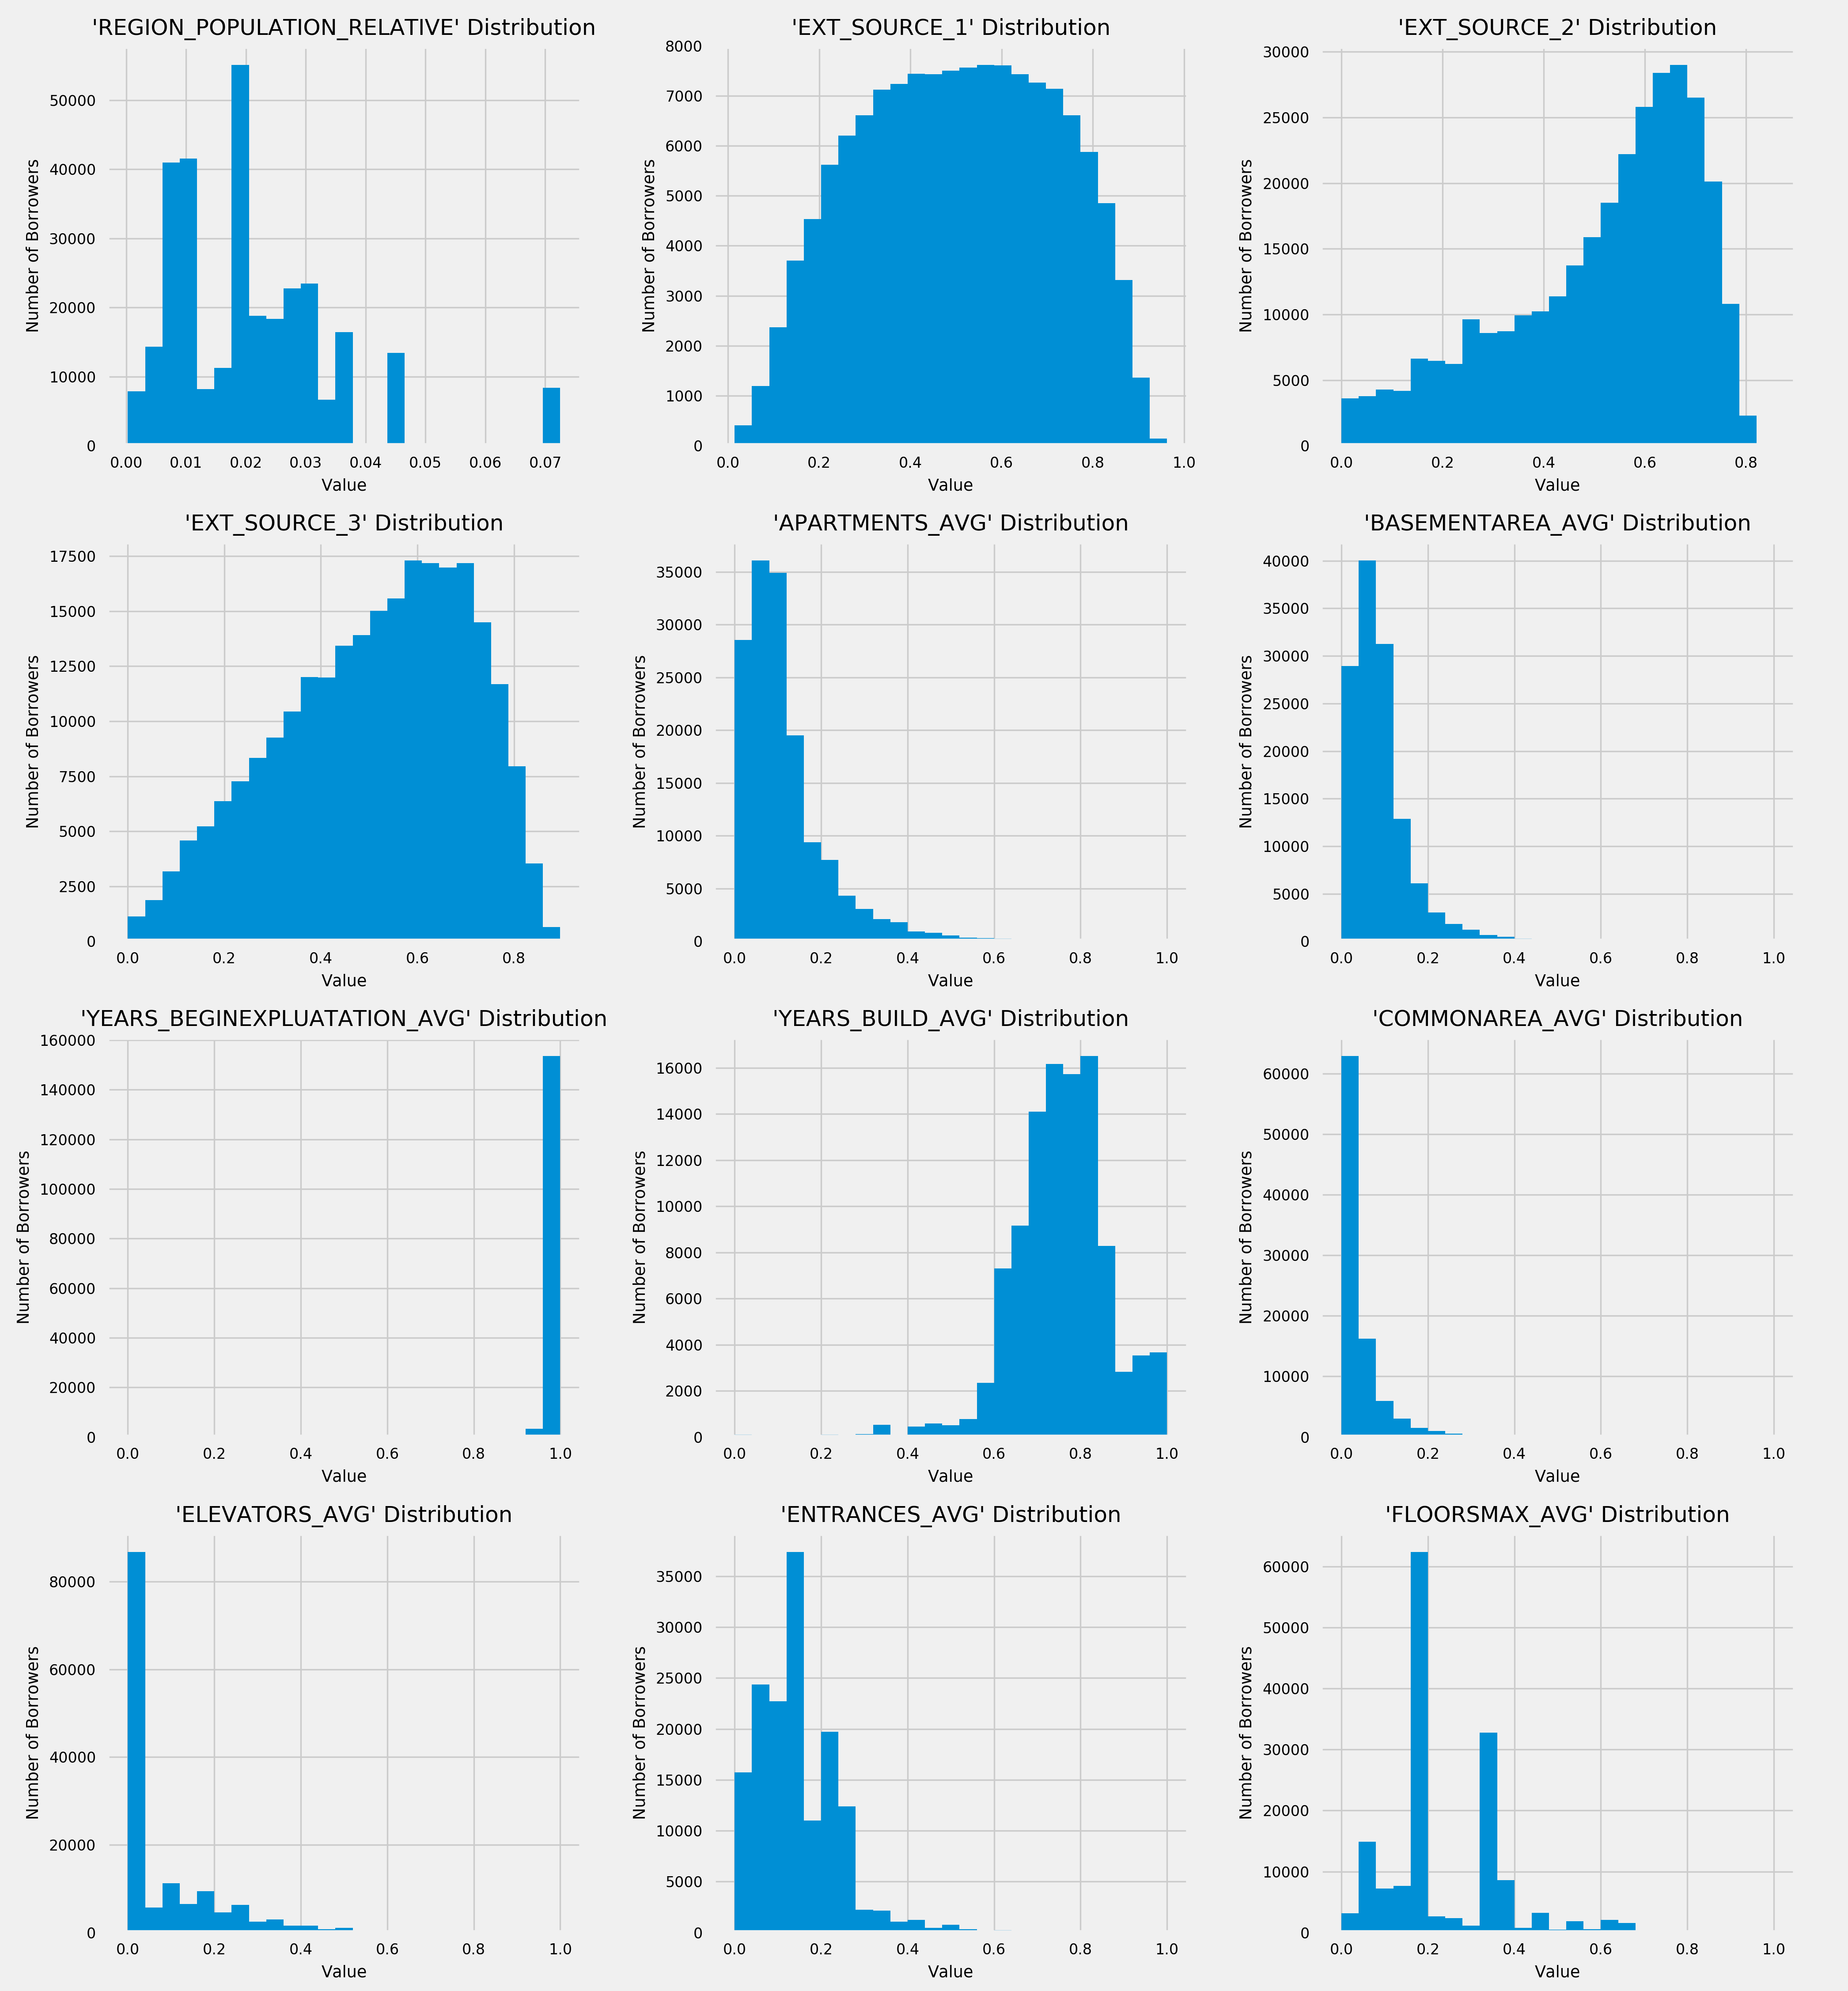
\includegraphics[width=0.89\textwidth]{main-data-table-normal-feature-distribs-p1}
\centering
\caption{Main Data Table Normalized Feature Distributions(1/4)}
\end{figure}

\pagebreak

\begin{figure}[ht]
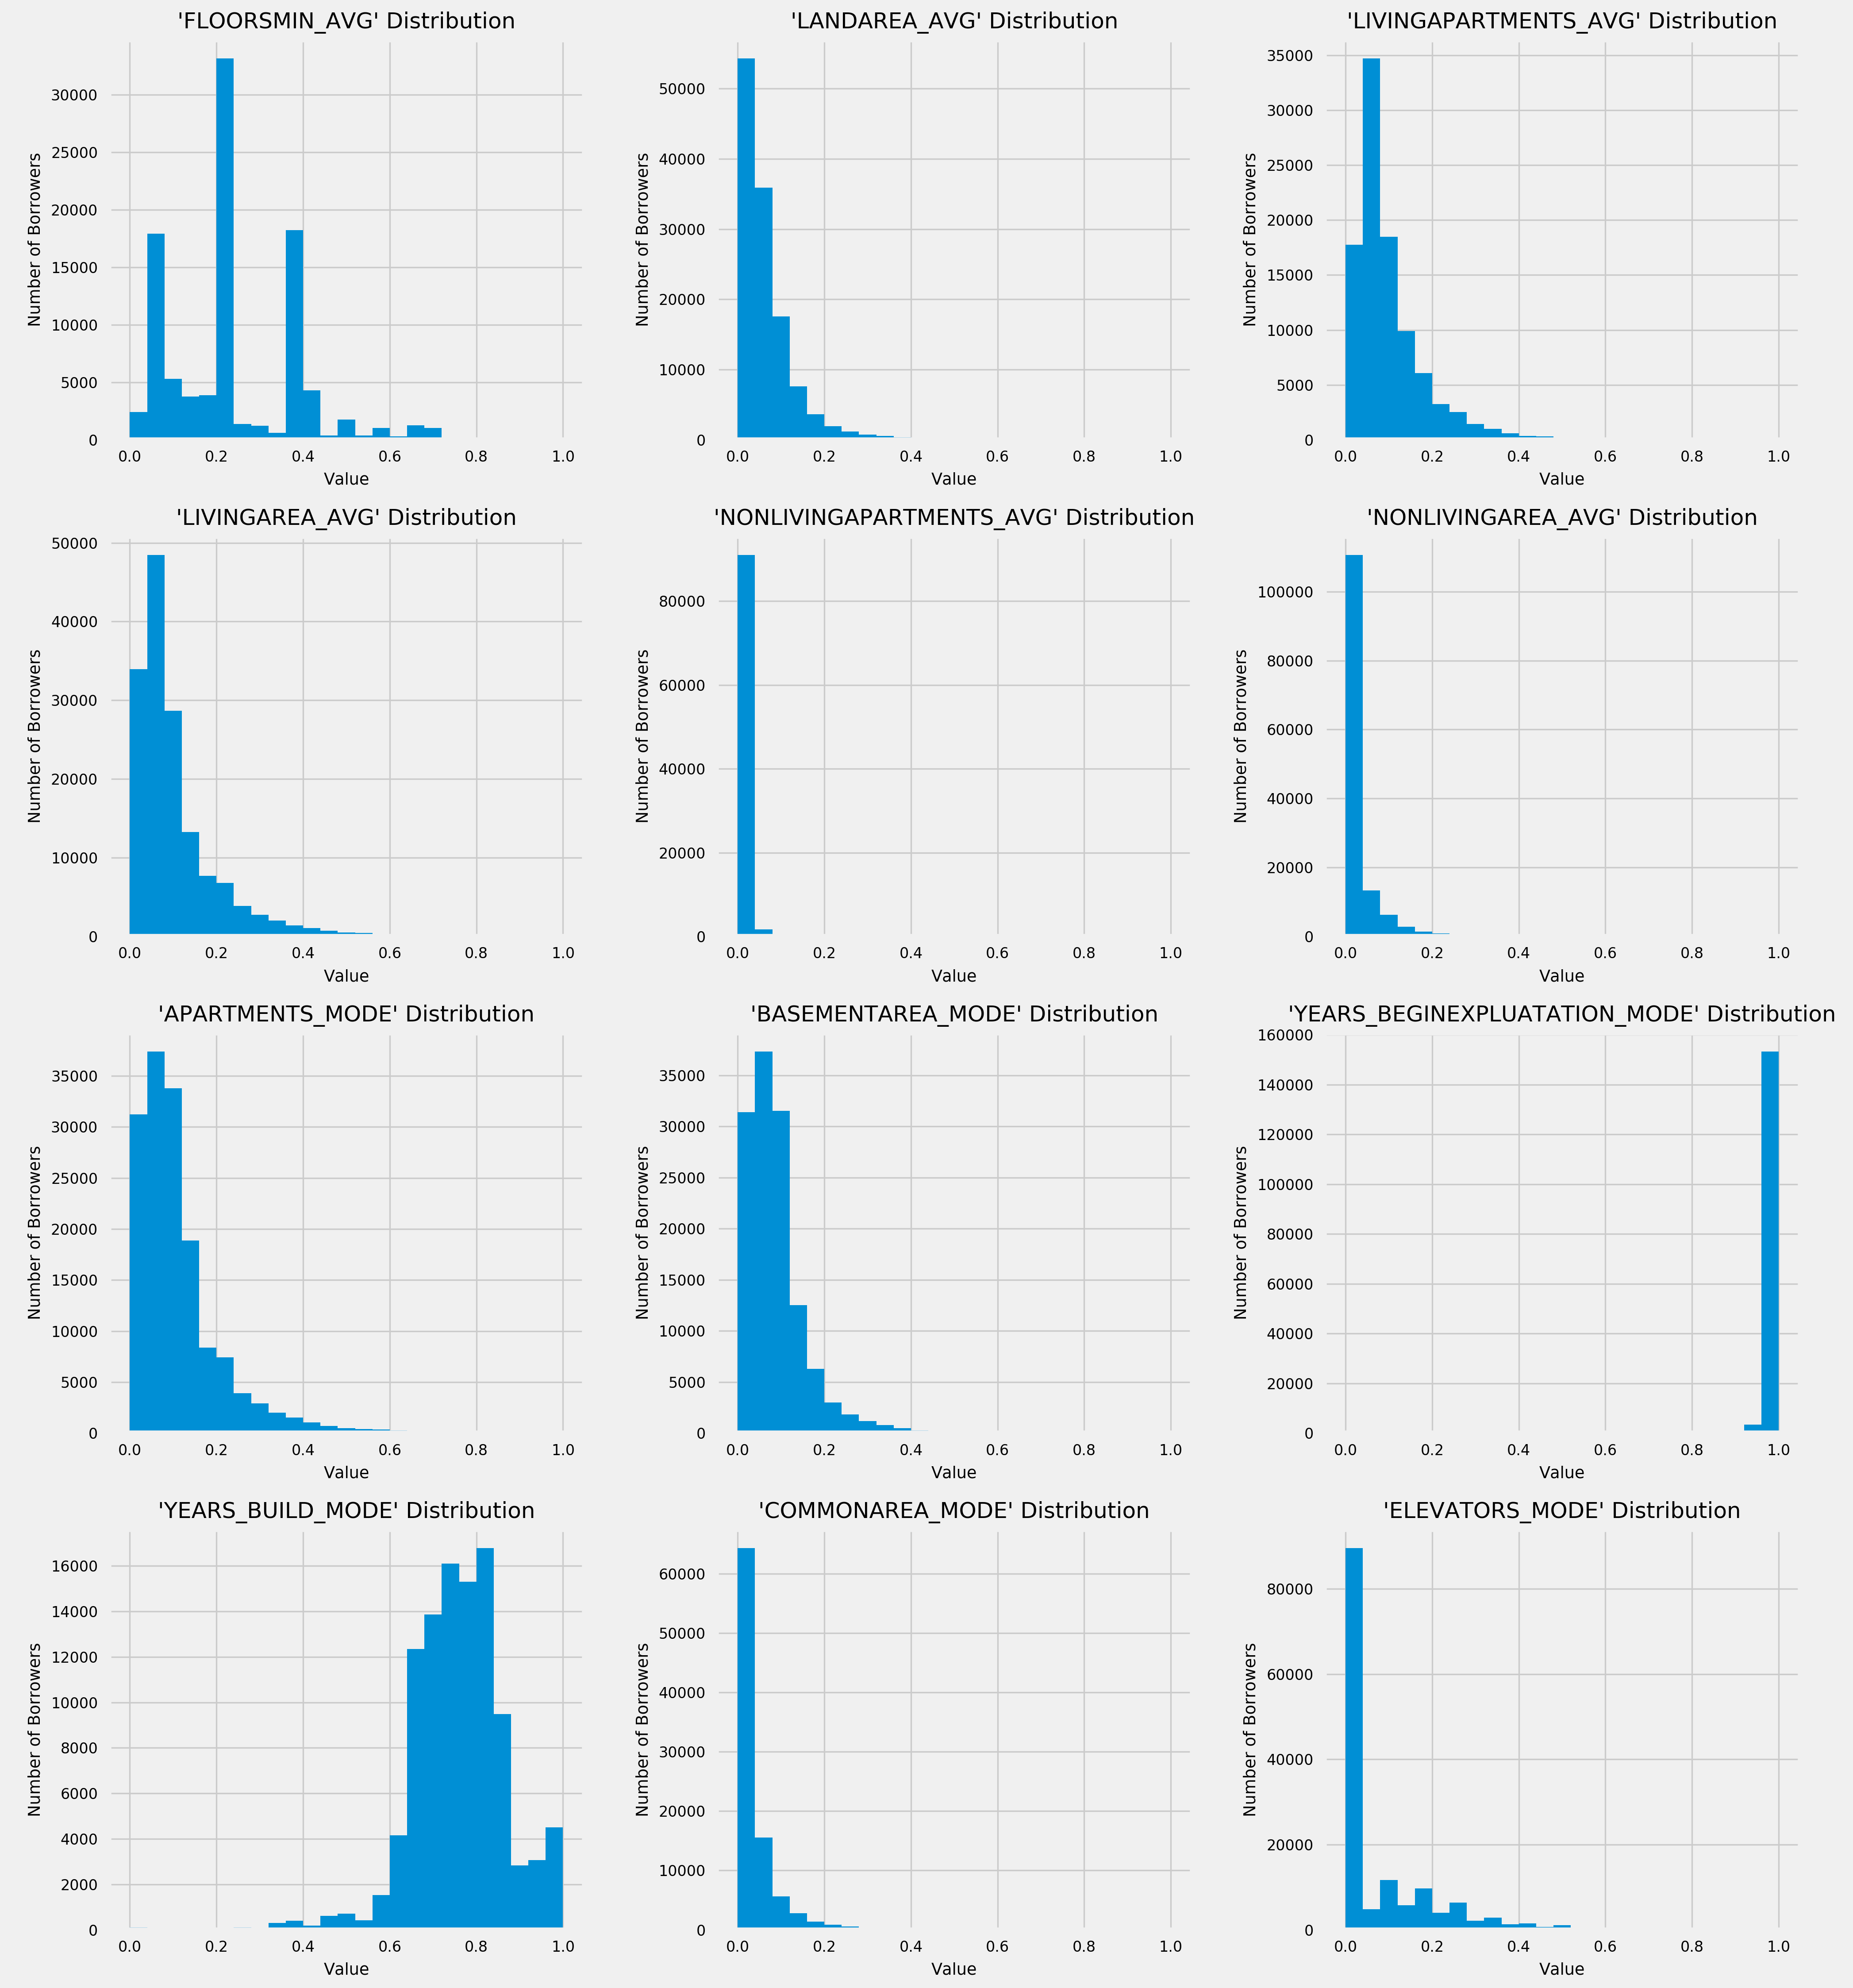
\includegraphics[width=0.89\textwidth]{main-data-table-normal-feature-distribs-p2}
\centering
\caption{Main Data Table Normalized Feature Distributions(2/4)}
\end{figure}

\pagebreak

\begin{figure}[ht]
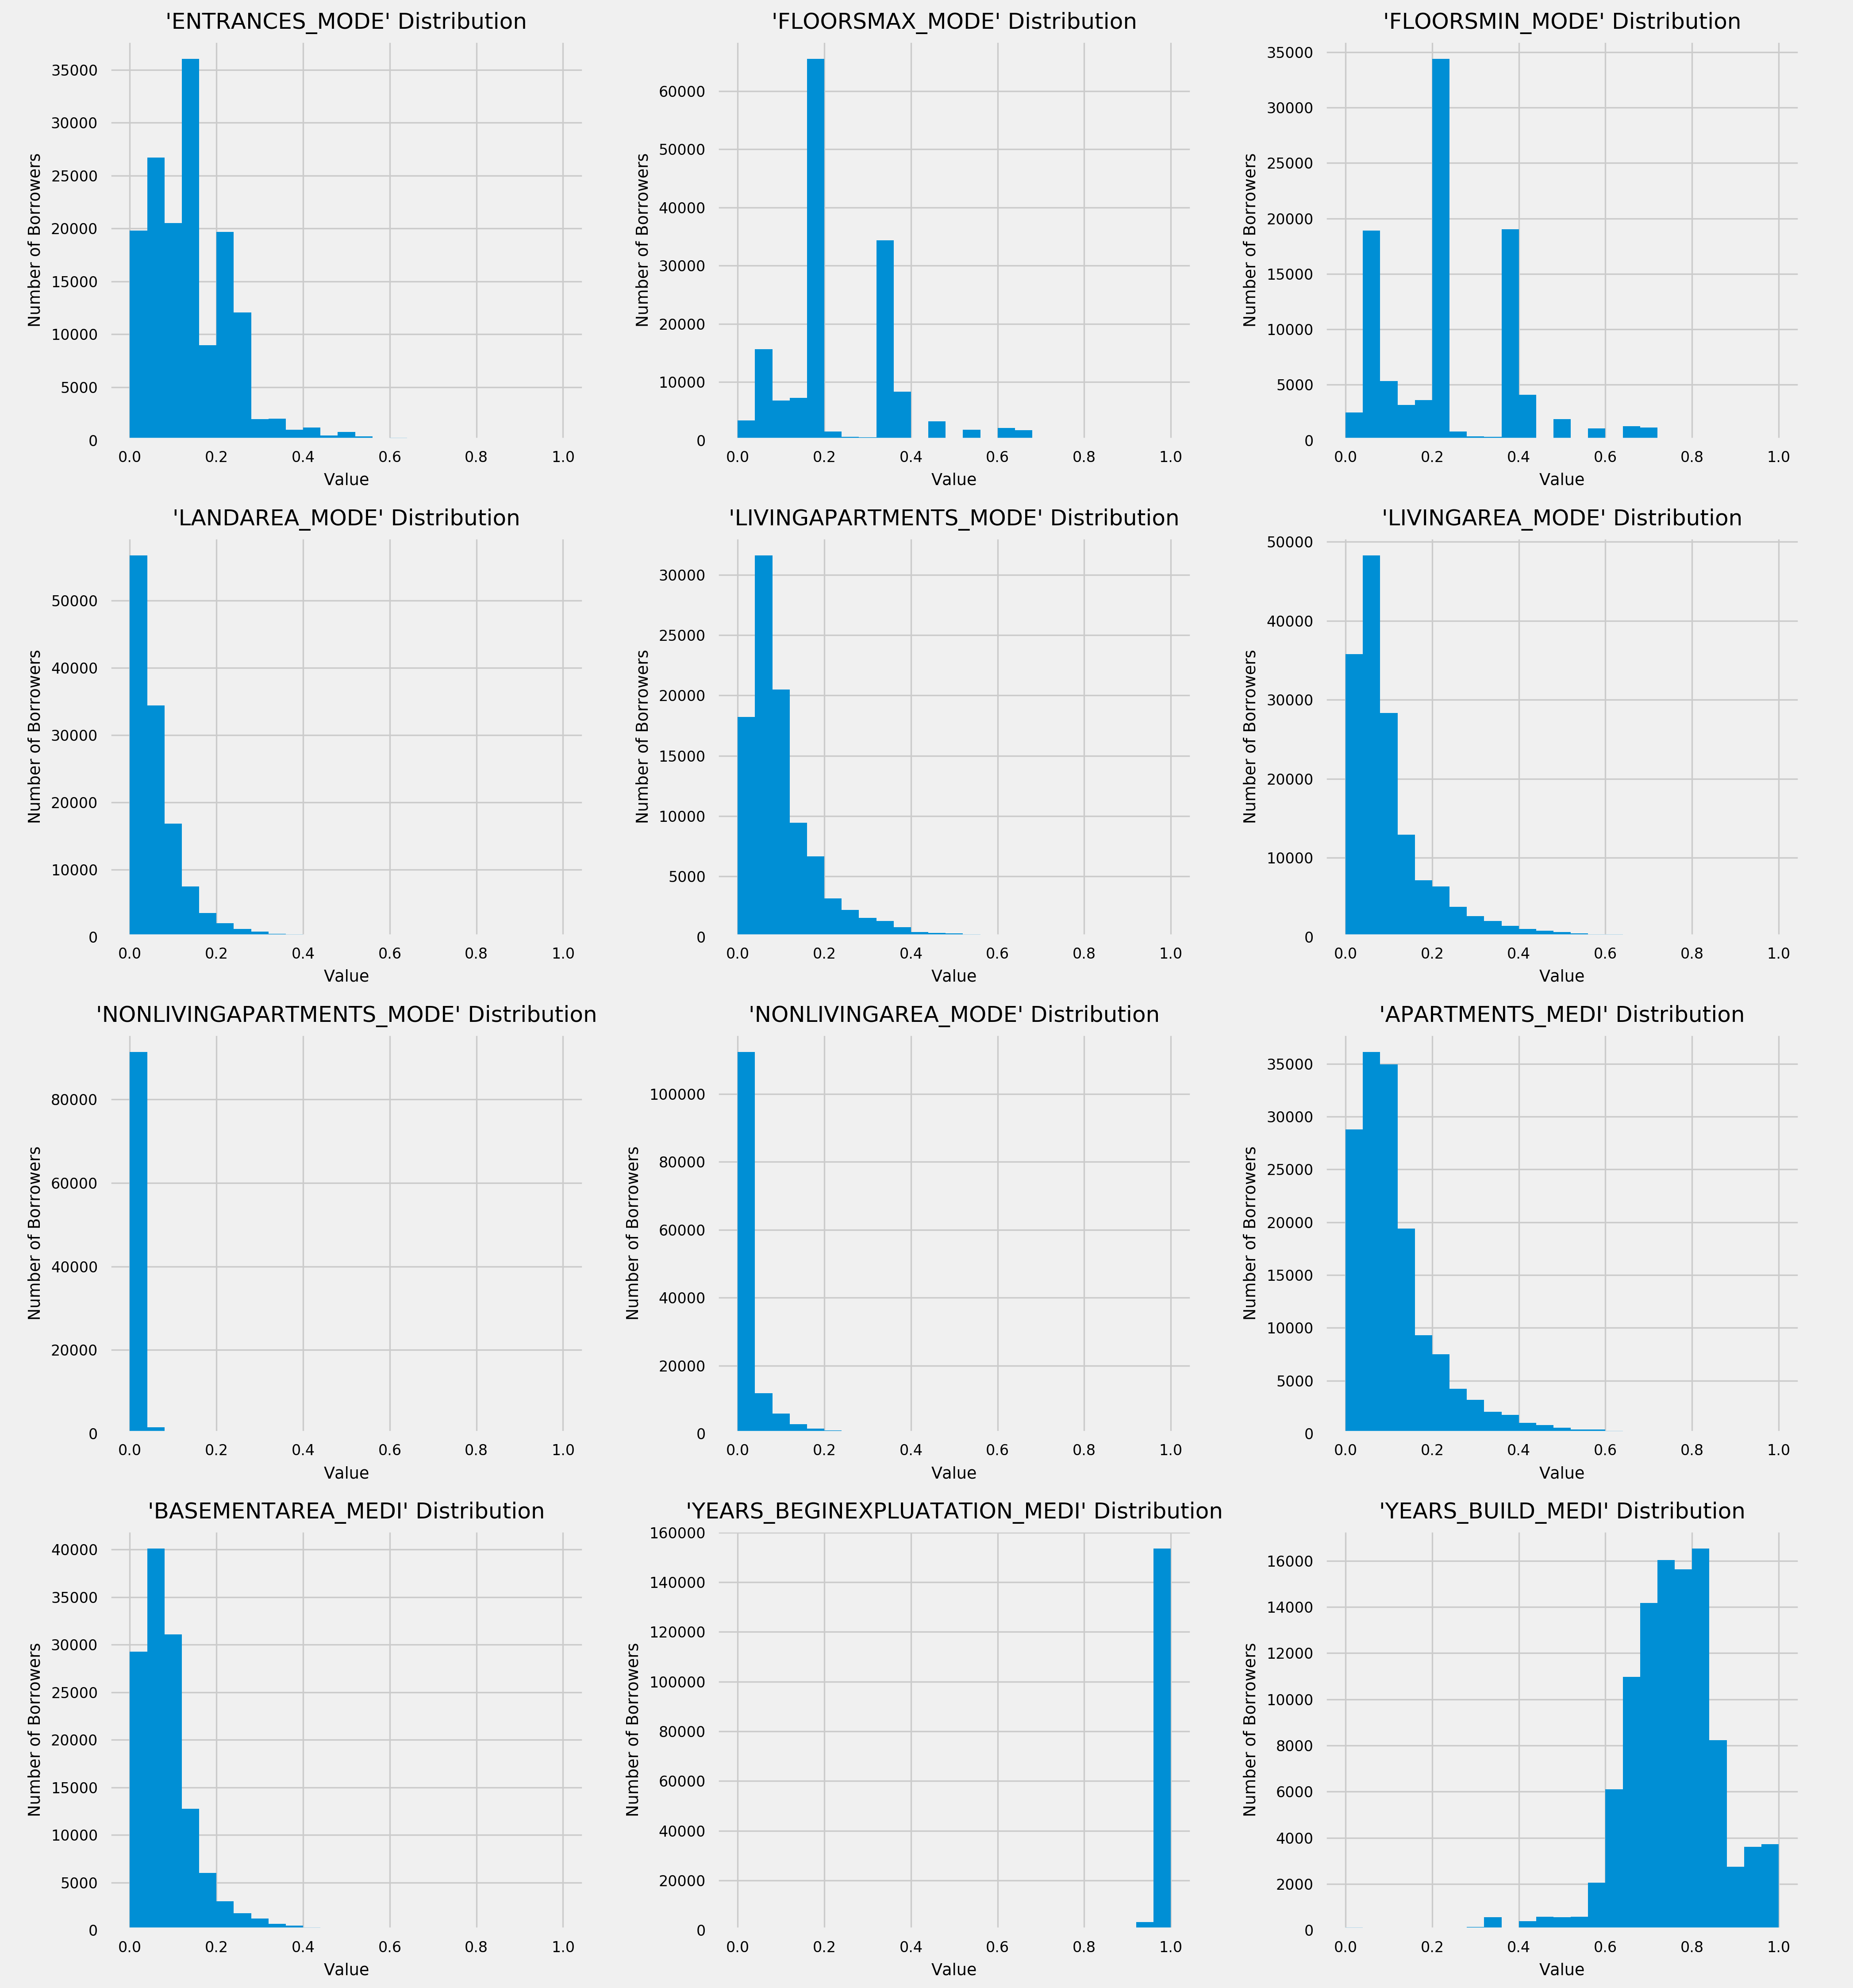
\includegraphics[width=0.89\textwidth]{main-data-table-normal-feature-distribs-p3}
\centering
\caption{Main Data Table Normalized Feature Distributions(3/4)}
\end{figure}

\pagebreak

\begin{figure}[ht]
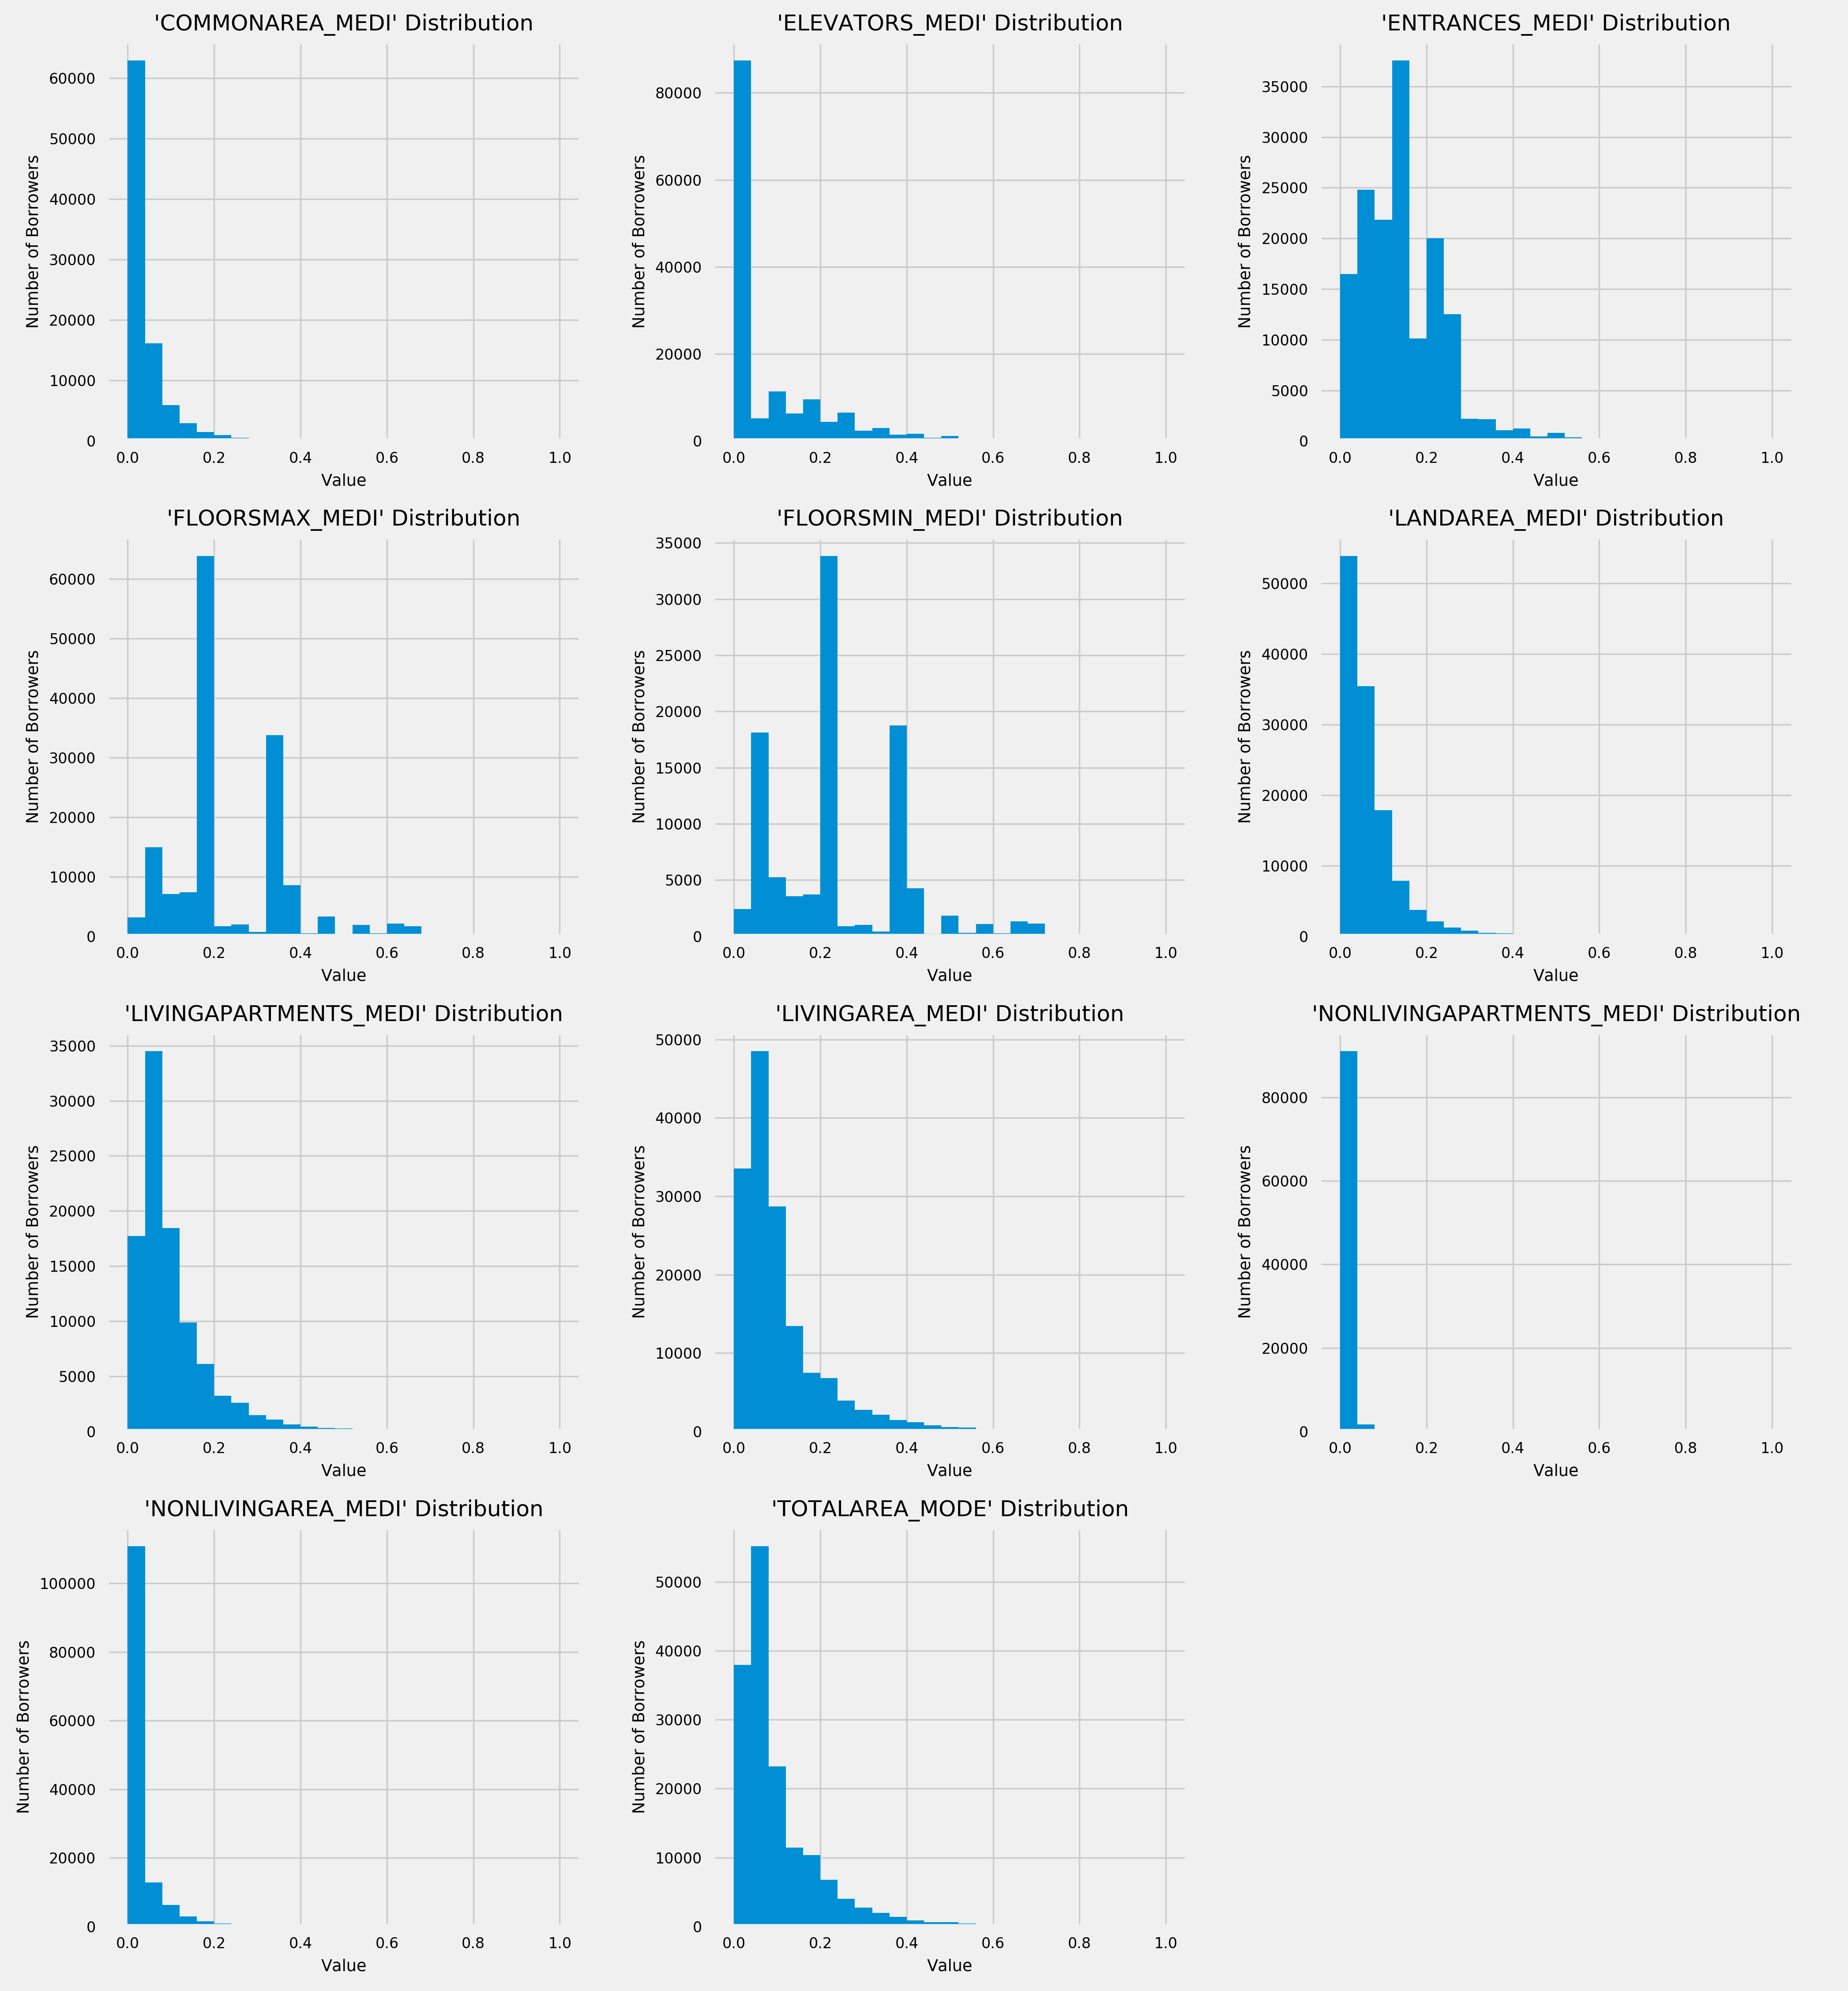
\includegraphics[width=0.89\textwidth]{main-data-table-normal-feature-distribs-p4}
\centering
\caption{Main Data Table Normalized Feature Distributions(4/4)}
\end{figure}

\pagebreak

\subsection{Main Data Table Non-normalized Feature Distributions}
\label{nonnormalfeaturedistribs}

\begin{figure}[ht]
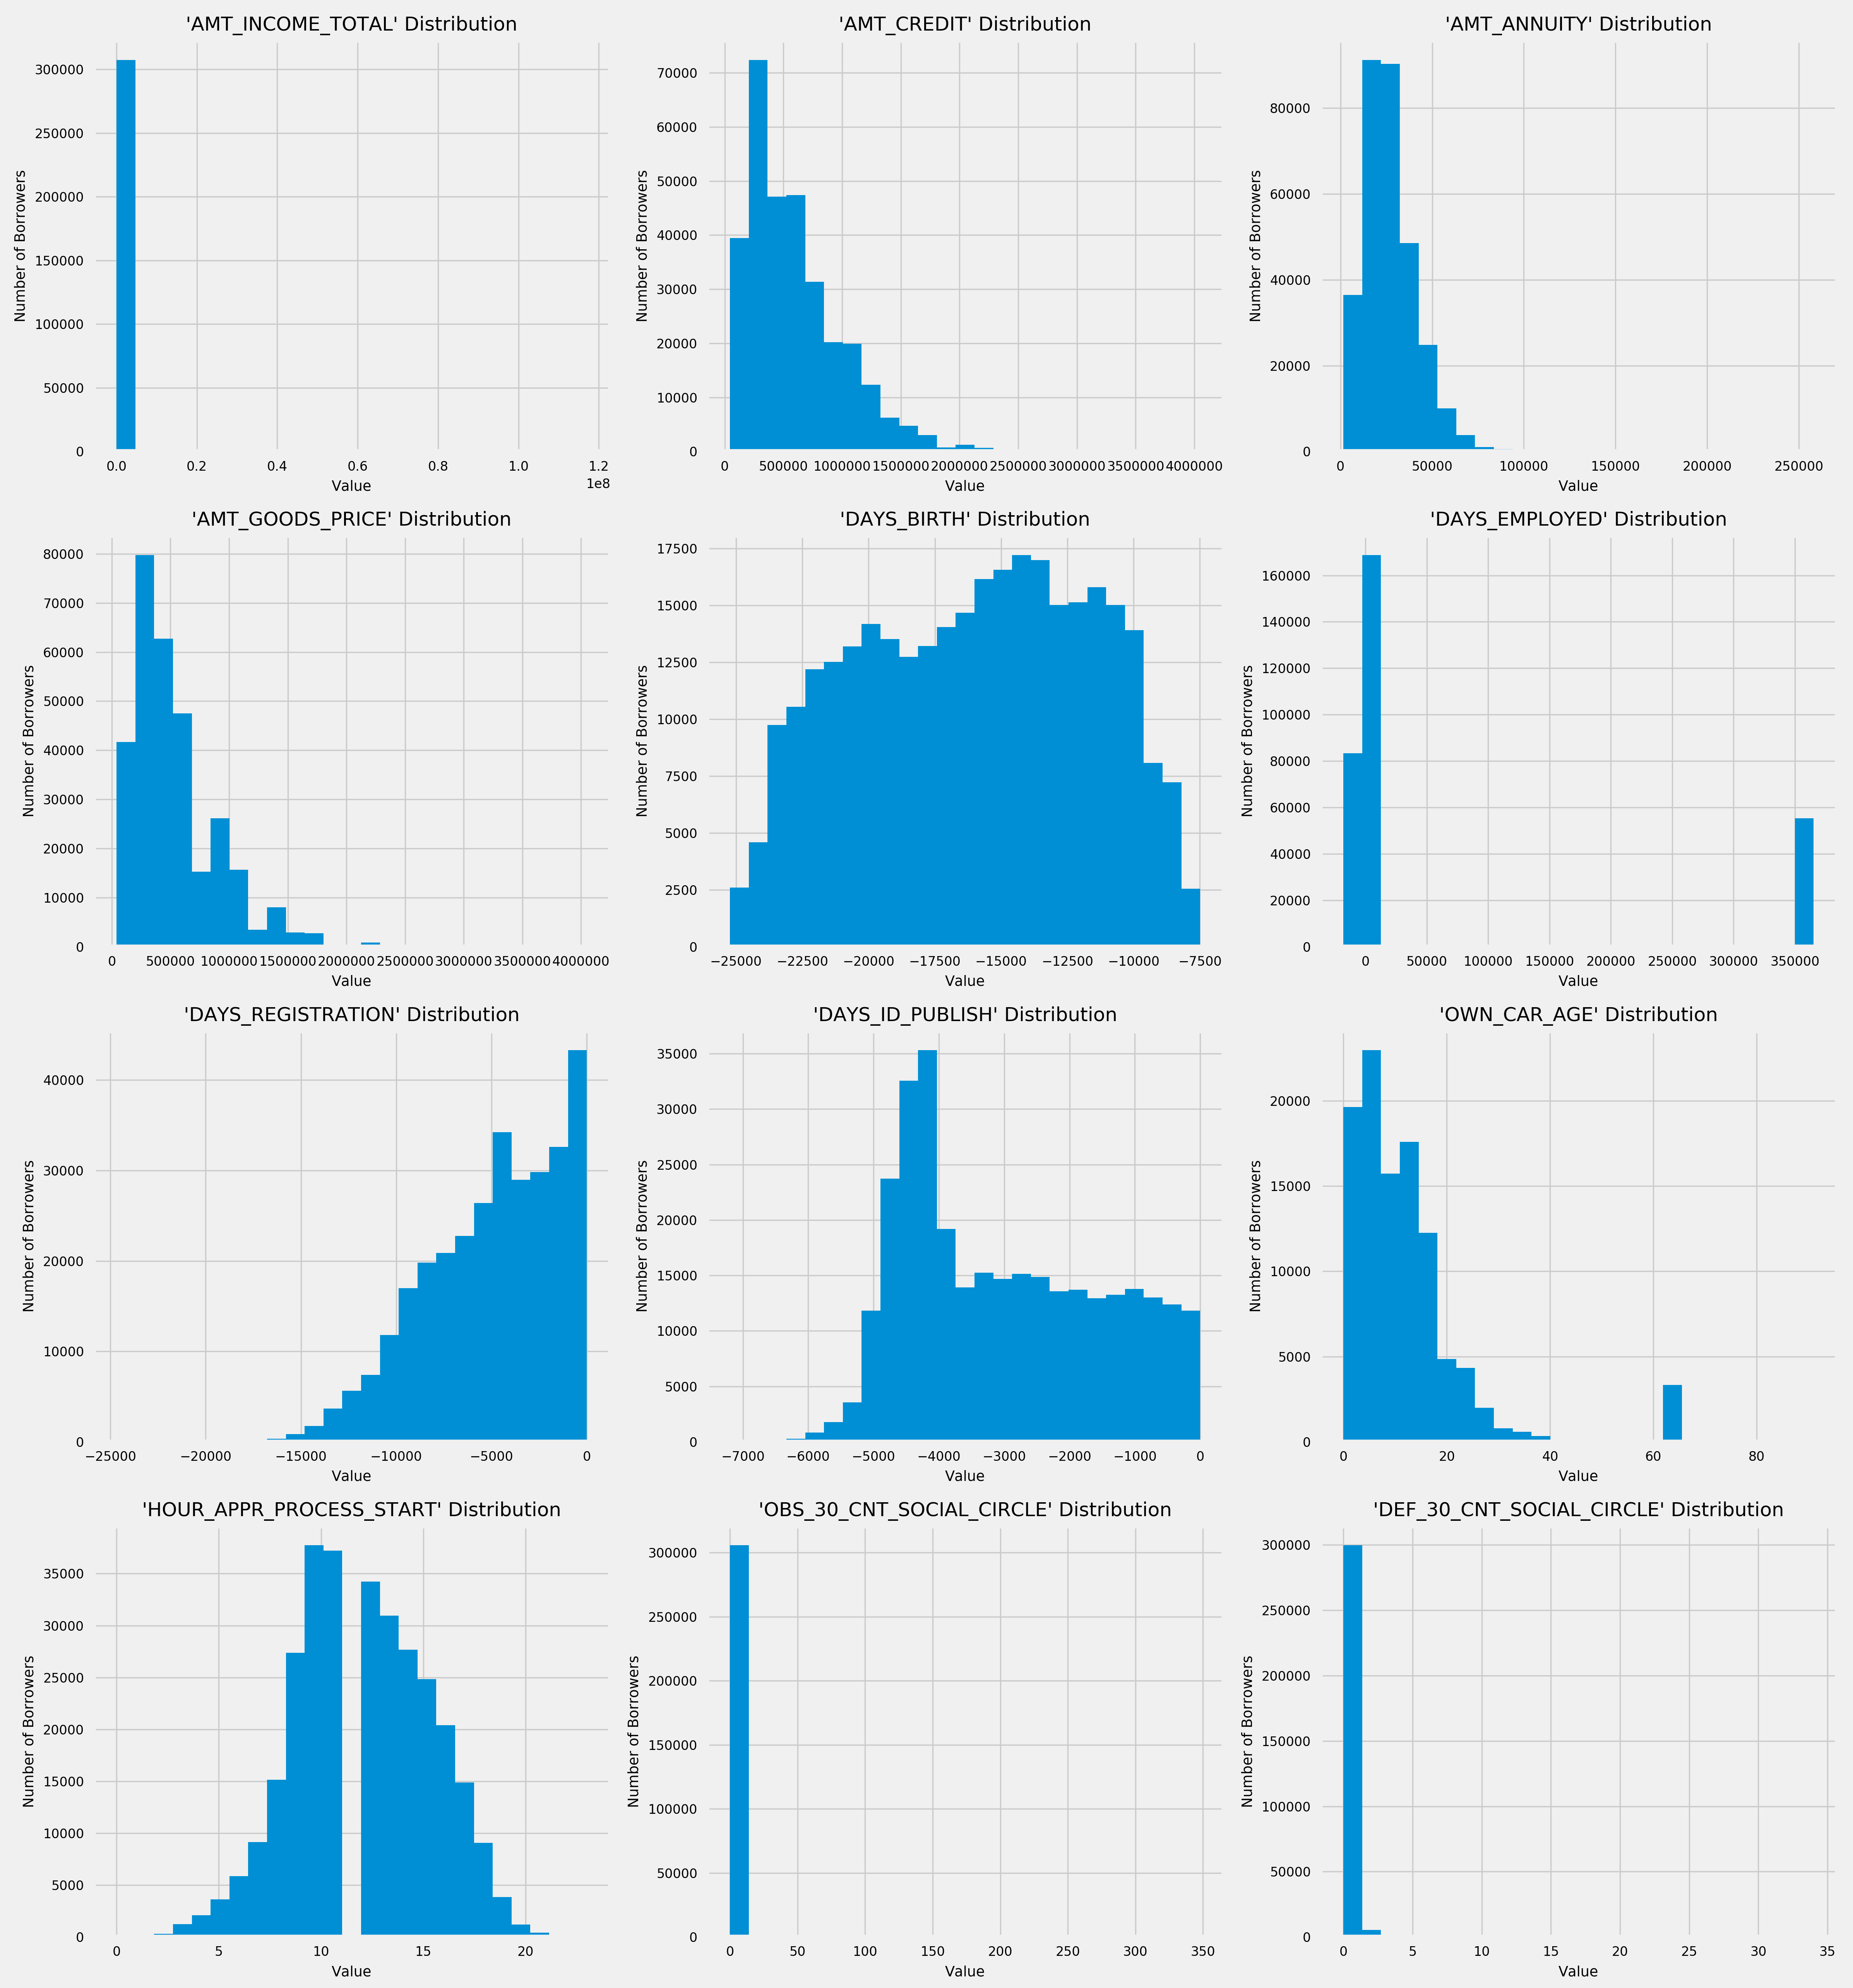
\includegraphics[width=0.89\textwidth]{main-data-table-non-normal-feature-distribs-p1}
\centering
\caption{Main Data Table Non-Normalized Feature Distributions(1/2)}
\end{figure}

\pagebreak

\begin{figure}[ht]
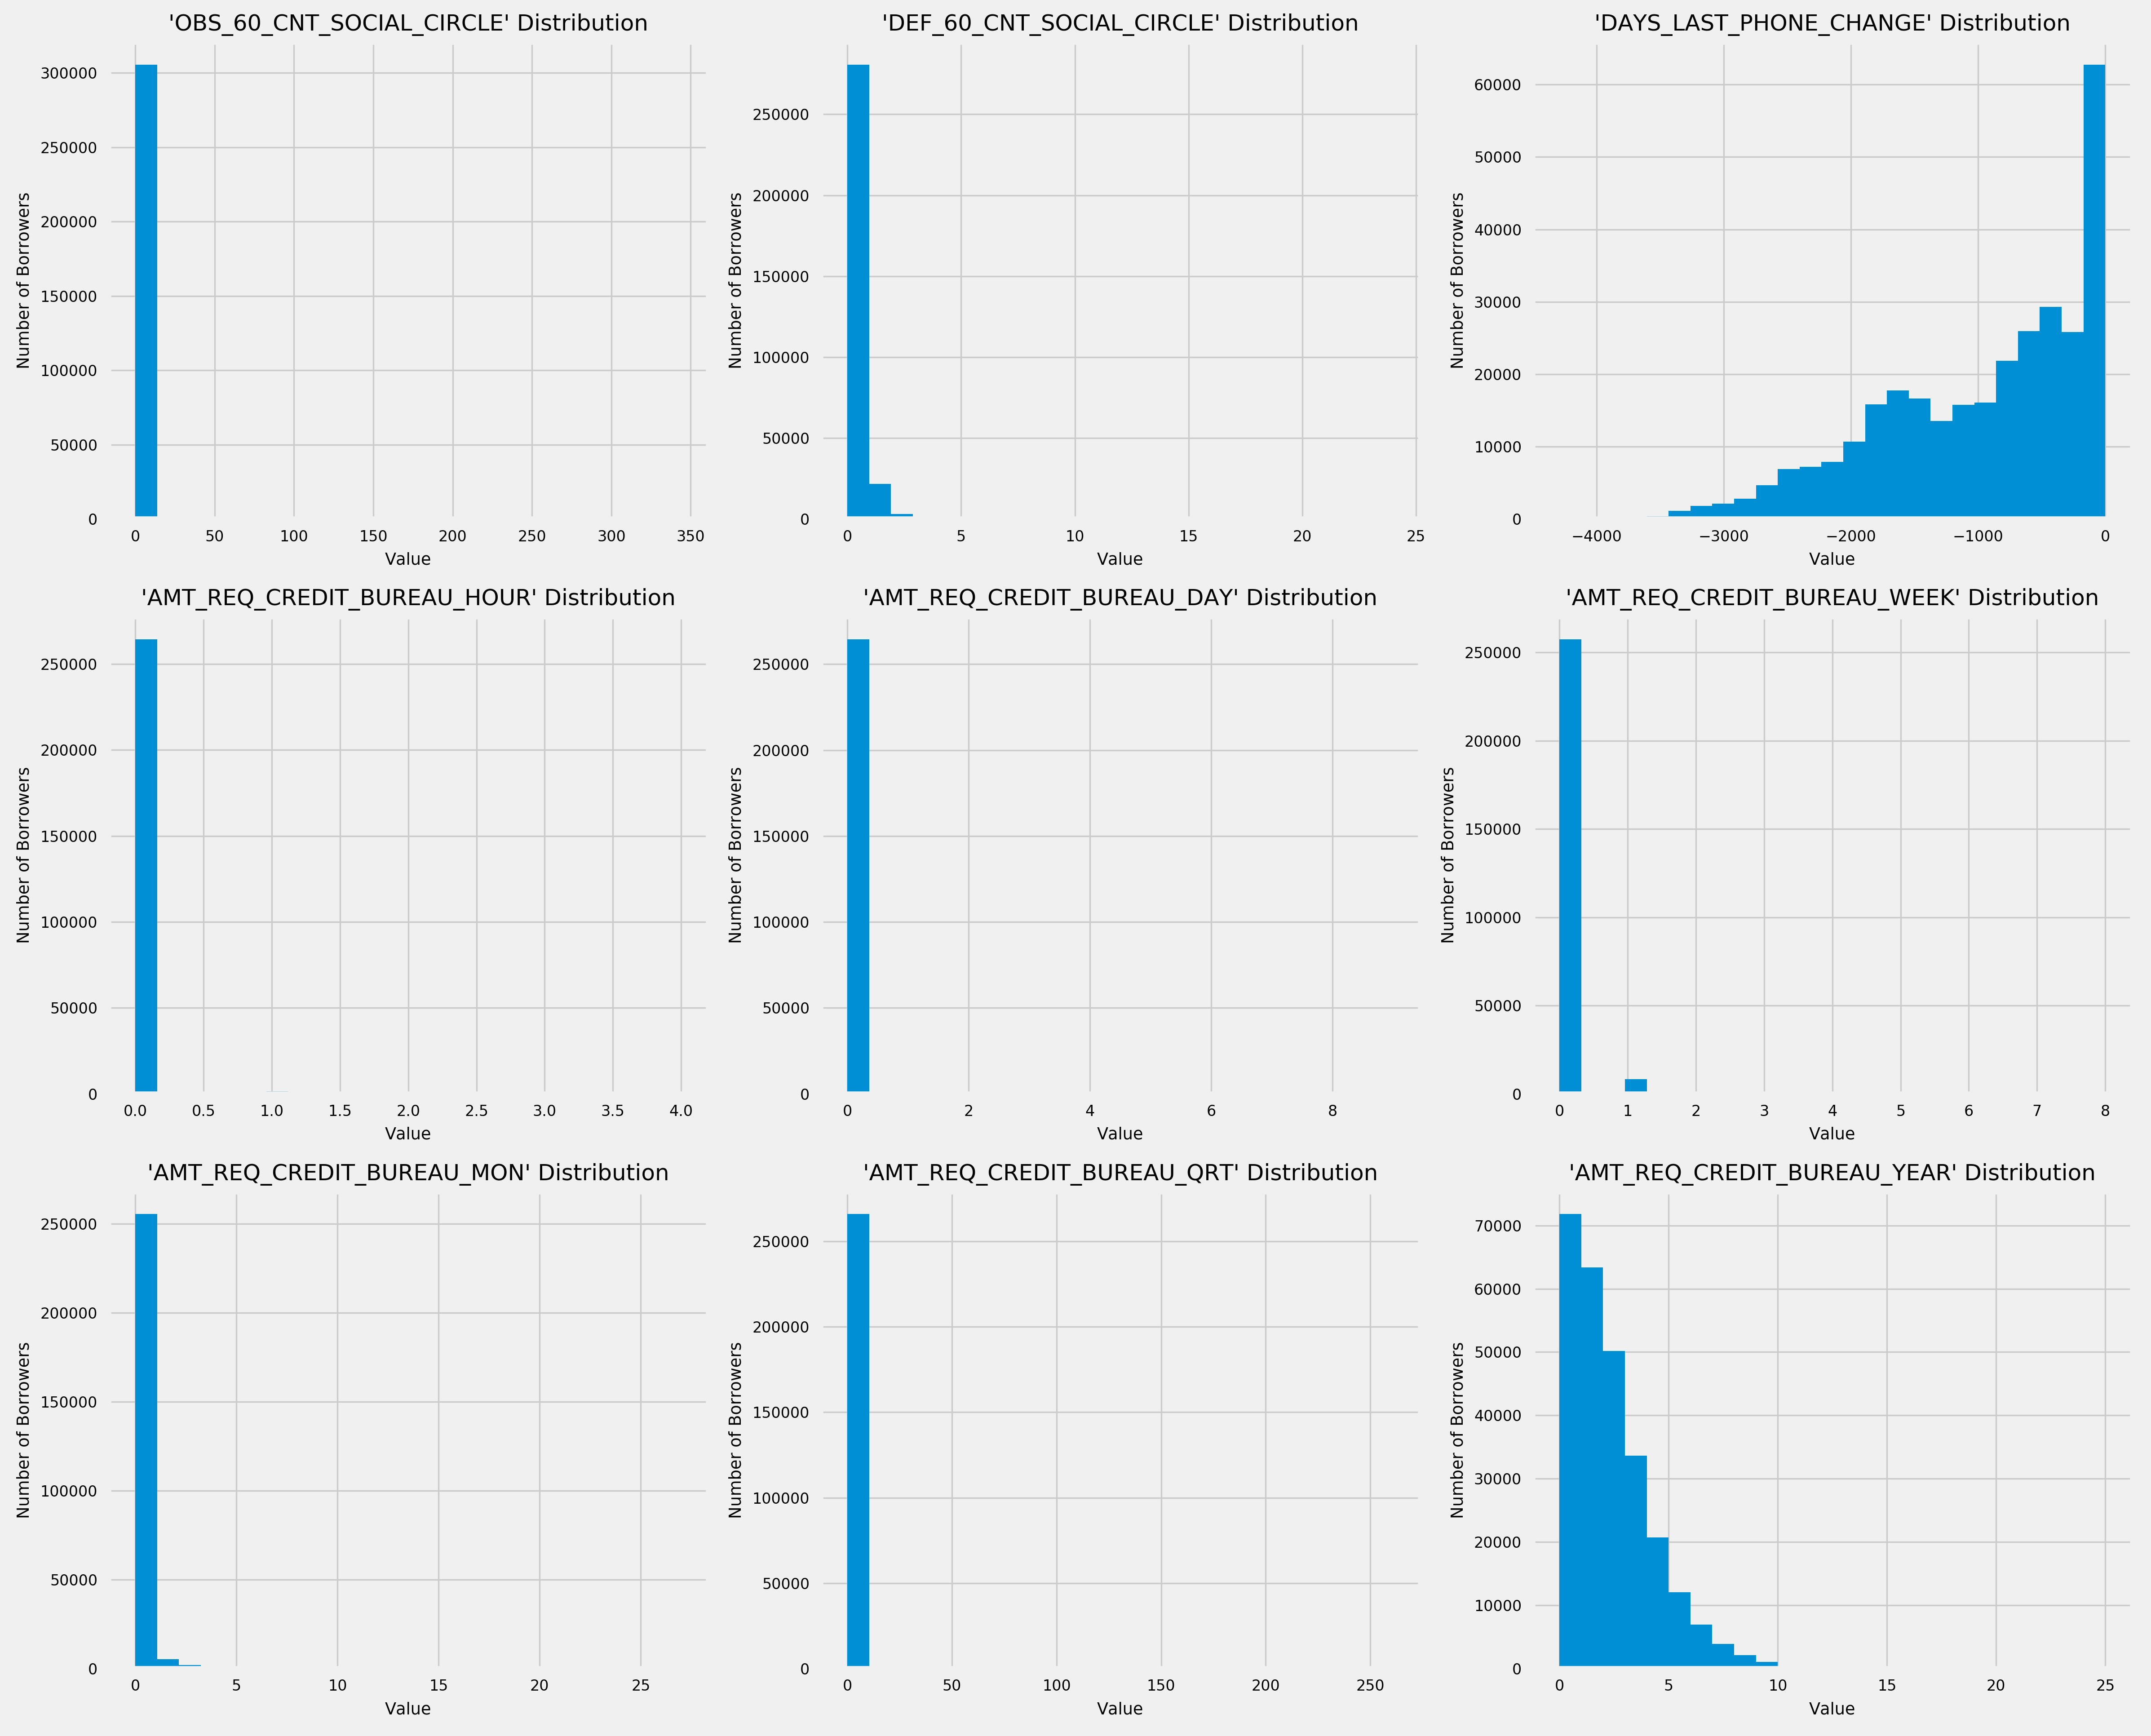
\includegraphics[width=0.89\textwidth]{main-data-table-non-normal-feature-distribs-p2}
\centering
\caption{Main Data Table Non-Normalized Feature Distributions(2/2)}
\end{figure}

\pagebreak

\end{appendices}

\printbibliography
\end{document}
